\documentclass[12pt,a4paper]{report}

\usepackage[T1]{fontenc}
\usepackage[utf8]{inputenc}
\usepackage{lmodern}
\usepackage{geometry}
\usepackage{setspace}
\usepackage{amsmath}
\usepackage{booktabs}
\usepackage{longtable}
\usepackage{graphicx}
\usepackage{float}
\usepackage{hyperref}
\usepackage{amsfonts}
\usepackage{csvsimple}

\geometry{margin=1in}
\onehalfspacing

\newcommand{\reportauthor}{Szymon Cichy 235093}

\title{Optimization Methods P\\ Starting Task - PFSP with EA \\ Friday 13:15 Project Group 2}
\author{\reportauthor}
\date{\today}

\begin{document}
\maketitle
\tableofcontents
\clearpage

\chapter{Introduction and Problem Definition}
\section{Motivation and Context}
PFSP is a standard combinatorial optimization problem used in production and scheduling.

For larger instances, exact methods are not practical because the search space grows factorially. This project focuses on an evolutionary algorithm (EA) and compares it with random search, greedy heuristics, and simulated annealing.

\section{Problem Statement}
In a standard PFSP setting:
\begin{itemize}
	\item processing times are known and fixed,
	\item each machine processes at most one job at a time,
	\item each job is processed by at most one machine at a time,
	\item no preemption is allowed (a job must be completed on a machine before it can move to the next),
    \item no passing is allowed (the order of jobs is the same on all machines).
\end{itemize}

In PFSP, all machines process jobs in one common permutation, so a solution is a permutation of jobs. The objective is to find a permutation that minimizes a given performance measure, such as Total Flow Time (TFT \(\sum C_j\)) or Makespan (\(C_{\max}\)).

\paragraph{Jobs and Machines.}
Jobs are indexed by $j\in \{1,\ldots,J\}$ and machines by $m\in \{1,\ldots,M\}$. Let $p(j,m)\ge 0$ denote the processing time of job $j$ on machine $m$. All jobs follow the same machine order $1,2,\ldots,M$.

\paragraph{Solution (Job Sequence).}
A job sequence $x = \langle x_1,\ldots,x_J\rangle$ is sought, where $x$ is a permutation of $\{1,\ldots,J\}$ specifying the order in which jobs are processed on every machine.

\paragraph{Completion times}
For a given sequence $x$, let $c(x_j,m)$ be the completion time of job $x_j$ on machine $m$ such that:
\begin{equation}
\label{eq:c-recurrence}
 c(x_j,m) =
 \begin{cases}
  p(x_j,m), & j=1 \land m=1,\\
  c(x_j,m-1) + p(x_j,m), & j=1 \land m>1,\\
  c(x_{j-1},m) + p(x_j,m), & j>1 \land m=1,\\
  \max\{c(x_{j-1},m),\; c(x_j,m-1)\} + p(x_j,m), & j>1 \land m>1~. 
 \end{cases}
\end{equation}

\paragraph{Objective (Total Flow Time).}
Many PFSP studies optimize makespan \(C_{\max}\). In this report, Total Flow Time (TFT), the sum of job completion times, is optimized.

The Total Flow Time for a given sequence $x$ can be expressed as:
\[
\mathrm{TFT} = f(x) = \sum_{j=1}^{J} c(x_j, M).
\]

Let $C_j := c(x_j,M)$ denote the completion time of the $j$th job in the sequence on the last machine M. Then $\mathrm{TFT} = \sum_{j=1}^{J} C_j$ The optimization problem can then be formally stated as:
\begin{equation}
 \min_{x \in \mathcal{S}_J} \; f(x) = \min \sum_{j=1}^{J} C_j,
\end{equation}
where $\mathcal{S}_J$ denotes all schedules (permutations) of jobs $\{1,\ldots,J\}$.\footnote{For $M\ge 2$ the problem is NP-hard. Lower values mean shorter average completion time.}. 


\chapter{Experimental Setup and Benchmark Instances}
\section{Benchmark Instances}
All experiments use six default Taillard PFSP instances from
\href{https://github.com/chneau/go-taillard}{github.com/chneau/go-taillard}.
The same instances are used in all comparisons. Results are reported by filename and size $(n,m)$, with comparison to best-known values.\\

\begin{longtable}{llrr}
\caption{Benchmark instances used in the experiments}\label{tab:bench_instances}\\
\toprule
Description & Filename & $n$ & $m$ \\
\midrule
\endfirsthead
\toprule
Description & Filename & $n$ & $m$ \\
\midrule
\endhead
Small instance 1 & \texttt{tai\_20\_5\_0} & 20 & 5 \\
Small instance 2 & \texttt{tai\_20\_10\_0} & 20 & 10 \\
Small instance 3 & \texttt{tai\_20\_20\_0} & 20 & 20 \\
Medium instance 1 & \texttt{tai\_100\_10\_0} & 100 & 10 \\
Medium instance 2 & \texttt{tai\_100\_20\_0} & 100 & 20 \\
Large instance 1 & \texttt{tai\_500\_20\_0} & 500 & 20 \\
\bottomrule
\end{longtable}

\section{Hardware and Software Environment}

\begin{longtable}{ll}
\caption{Hardware and software environment for reproducibility}\label{tab:hardware_software}\\
\toprule
Item & Value \\
\midrule
\endfirsthead
\toprule
Item & Value \\
\midrule
\endhead
CPU & AMD Ryzen 7 9800X3D \\
Cores/Threads & 8 / 16 \\
RAM & 64\,GB \\
Operating System & Windows 11 \\
Python Environment & Python 3.13.12; uv-managed virtual environment\\
Python Libraries & matplotlib $\ge 3.10.8$; notebook $< 7$; pandas $\ge 3.0.1$; scipy $\ge 1.17.1$ \\
C\# / .NET SDK & Microsoft.NET.Sdk; TargetFramework: net10.0\\
NuGet Packages & BenchmarkDotNet 0.15.2; BenchmarkDotNetDiagnosers; Newtonsoft.Json 13.0.3 \\
Parallelism & Only parallel experiments, no algorithm-level parallelism \\
\bottomrule
\end{longtable}


\section{Evaluation Protocol}

\begin{itemize}
    \item The stopping criterion was first defined.
    \item The EA budget was calibrated with a population-size \(\times\) generations sweep and then aggregated by number of evaluations; the final operating budget was selected pragmatically with respect to run time and expected sufficiency.
    \item For SA, one neighborhood operator was selected using a one-run comparison.
    \item A base comparison of all algorithms with default parameters was then performed.
    \item EA parameter analysis was then conducted on all instances, including one-dimensional and two-dimensional sweeps, per-instance performance analysis, and run-dynamics analysis for selected settings.
    \item Based on those analyses, parameter values were fixed for subsequent experiments.
    \item Ablation and operator-comparison studies were then performed.
    \item Finally, a full comparison against the other algorithms was executed using the final EA configuration.
    \item Improvement relative to the base/default parameterization was recorded.
\end{itemize}


\subsection{Protocol Justification}
This process should ensure fair comparison with minimal complexity. A common budget is used to make comparisons algorithmically fair. Seeding choice should make the experiments reproducible. Sample size should be a balance between capturing valid statistical variability and keeping computation time reasonable. Reporting both final quality and runtime traces shows effectiveness and algorithm behavior.

The protocol should deliver defensible results from the start and be extendable without changing the core design of the experiments or algorithms.


\subsection{Seeds and Samples}

\paragraph{Seeds} All stochastic runs use explicit seeds for reproducibility.

For each algorithm-instance-configuration combination, independent runs use:
\[
\text{seed}_i = (\text{base\_seed} \oplus (i\cdot 1\,000\,003)) \wedge 2\,147\,483\,647, \quad i \in 0,1,\dots,n-1.
\]

The first run uses the base seed directly (offset \(0\)).

\paragraph{Sample size} Experiments use a sample size of \textbf{n = 20}. Screening runs with fewer runs are not shown, but were used for parameter choice.

\subsection{Reported Metrics}
The report uses metrics emitted by the monitoring system and aggregated per configuration.

\paragraph{Core metrics for all algorithms.}
\begin{itemize}
    \item \textbf{Best solution cost} \(f_{best}\): final best objective value found in a run.
    \item \textbf{Evaluations}: total number of objective evaluations used in a run.
    \item \textbf{ElapsedMs}: wall-clock runtime in milliseconds.
    \item \textbf{BestFoundAtEvaluation}: evaluation index at which the final best was first found.
    \item \textbf{BestCostByEvaluation}: indexed best-so-far cost trace over evaluations.
\end{itemize}

\paragraph{EA generation metrics.}
\begin{itemize}
    \item \textbf{BestByGeneration}: best-so-far cost after each generation.
    \item \textbf{WorstByGeneration}:  worst-so-far cost after each generation.
    \item \textbf{BestInPopulationByGeneration}: best individual cost in the current generation.
    \item \textbf{WorstInPopulationByGeneration}: worst individual cost in the current generation.
    \item \textbf{MeanByGeneration}: mean population cost per generation.
    \item \textbf{DeviationByGeneration}: population standard deviation of cost per generation.
    \item \textbf{HammingDistanceByGeneration}: average pairwise Hamming distance in the population.
\end{itemize}


\paragraph{Aggregated statistics reported in tables and plots.}
Between-run statistics aggregated across the sample of runs for each configuration include:
\begin{itemize}
    \item \textbf{best}: minimum of run-level best costs,
    \item \textbf{mean}: arithmetic mean of run-level best costs,
    \item \textbf{worst}: maximum of run-level best costs,
    \item \textbf{std}: standard deviation of run-level best costs,
    \item \textbf{runtime}: summary of \texttt{ElapsedMs},
    \item \textbf{evaluation count}: summary of \texttt{Evaluations}.
\end{itemize}

\subsection{Stopping Criterion and Computational Budget}

\paragraph{Number of Fitness Evaluations (NFE).} It is a \textbf{maximum number of objective evaluations}. Let \(B\) be the per-run budget.

For the evolutionary algorithm with population size \(P\), generations \(G\), and elitism \(k\), the effective NFE is:
\[
B = P + (G - 1)\cdot(P-k).
\]
For \(k=0\), this simplifies to \(B = P\cdot G\).

The same NFE budget is used across methods for comparable search effort. Greedy methods are deterministic and return one solution per run.

\paragraph{Limitations} NFE is hardware-independent, but one evaluation may take different time across methods (e.g., caching, incremental updates, neighborhood generation). So this is an \emph{algorithmic} budget, not a runtime budget.

\paragraph{Alternatives} Wall-clock budgets or target-quality stopping criteria are possible, but they add hardware and implementation effects.

\subsection{Budget Calibration Procedure}

A single fixed budget \(B\) keeps the design simple and comparable, but it is a trade-off: small and large instances may need different effort.

Before the main study, a pilot Evolutionary algorithm test was run on default instances.

\subsubsection*{Population size vs Generations Parameter Sweep}
In this 2D sweep, solution quality is mapped over a grid of population size ($P$) and generations ($G$), and the study’s evaluation budget $B$ is chosen based on the revealed general tendencies across $(P,G)$. The exploration–exploitation trade-off (larger $P$ for diversity vs. larger $G$ for depth) is exposed, and regions of diminishing returns are surfaced.


\begin{figure}[H]
\centering
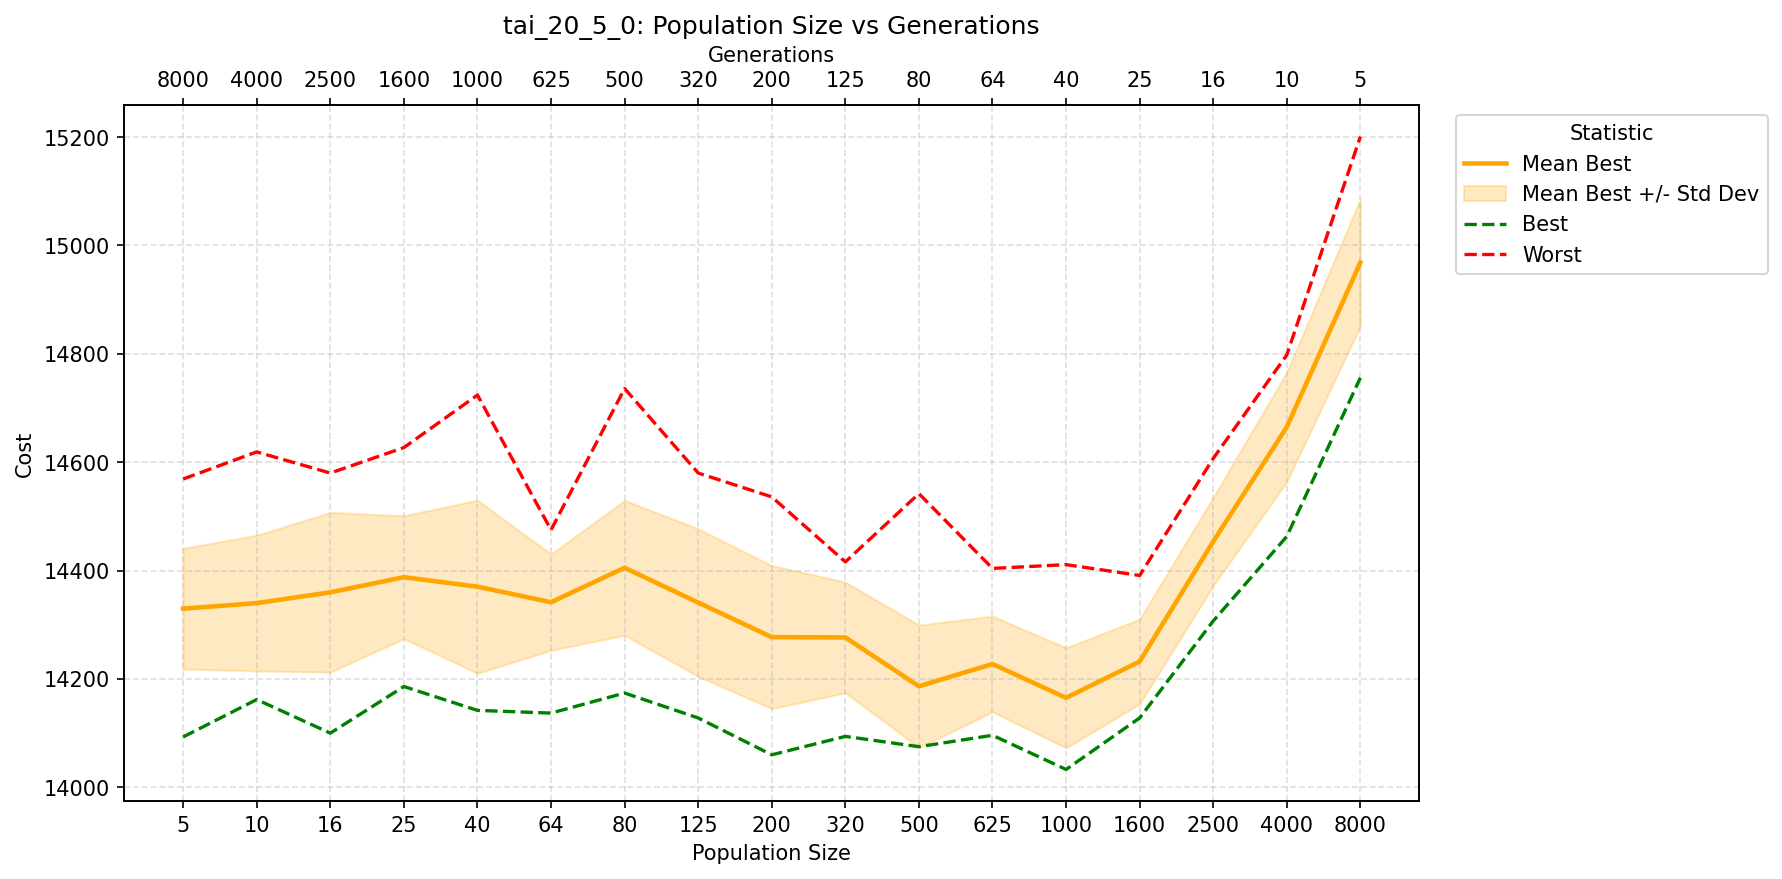
\includegraphics[width=0.48\textwidth]{../Experiments/01_default_evolutionary_population_generations/fig_tai_20_5_0.png}
\hfill
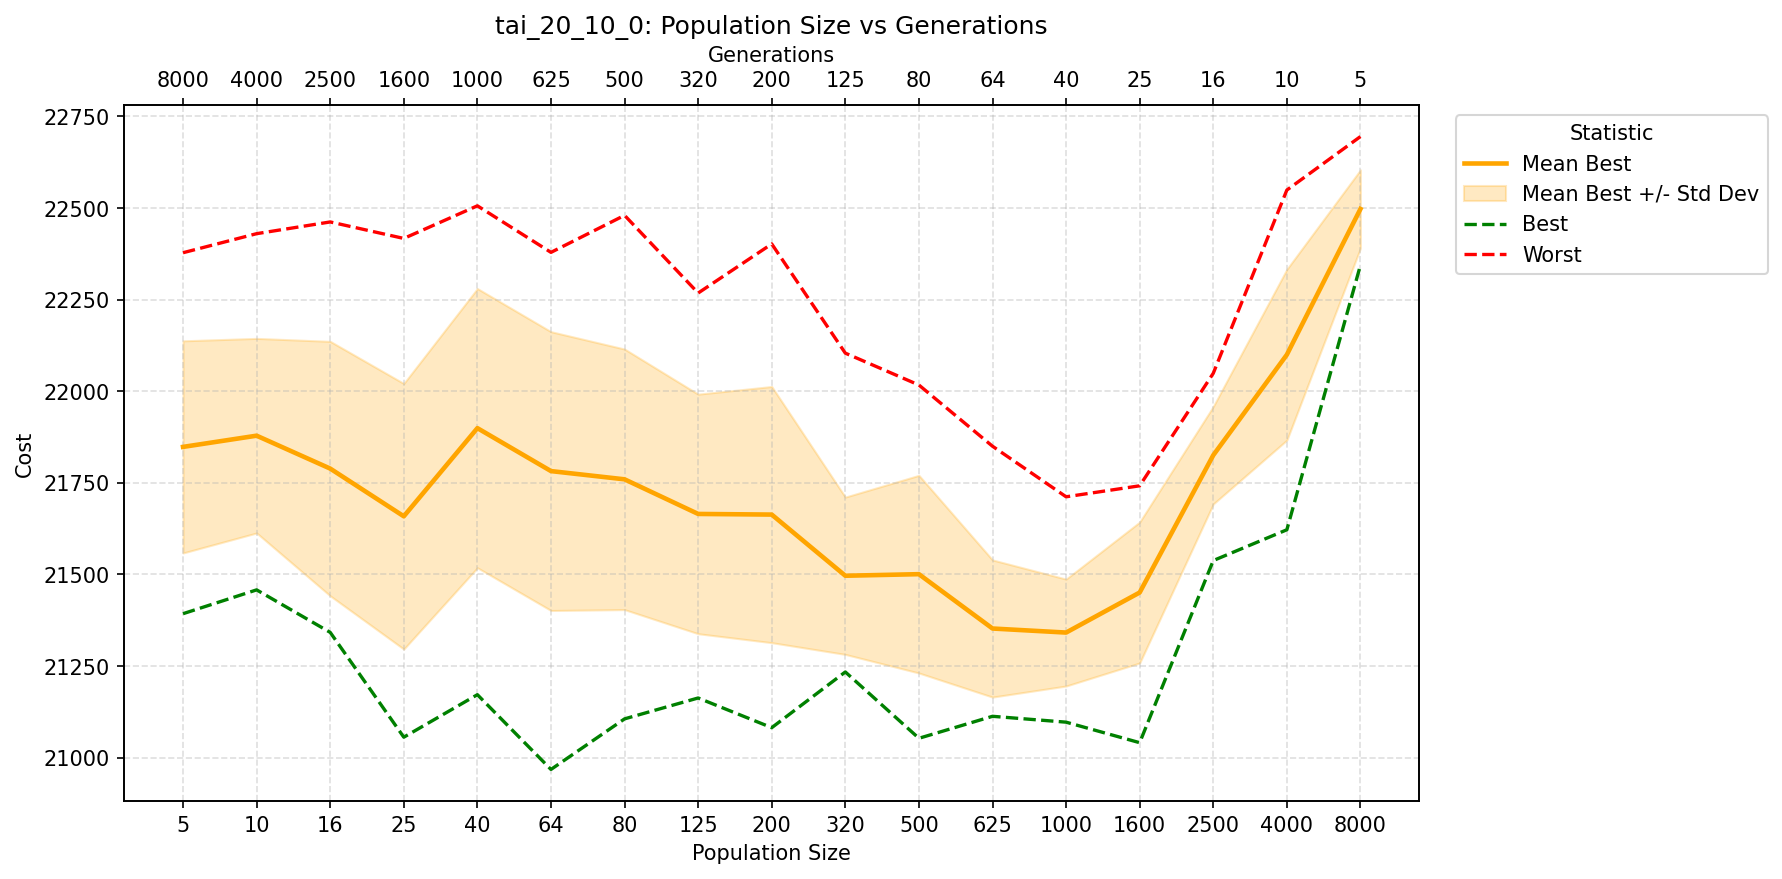
\includegraphics[width=0.48\textwidth]{../Experiments/01_default_evolutionary_population_generations/fig_tai_20_10_0.png}

\vspace{0.5em}

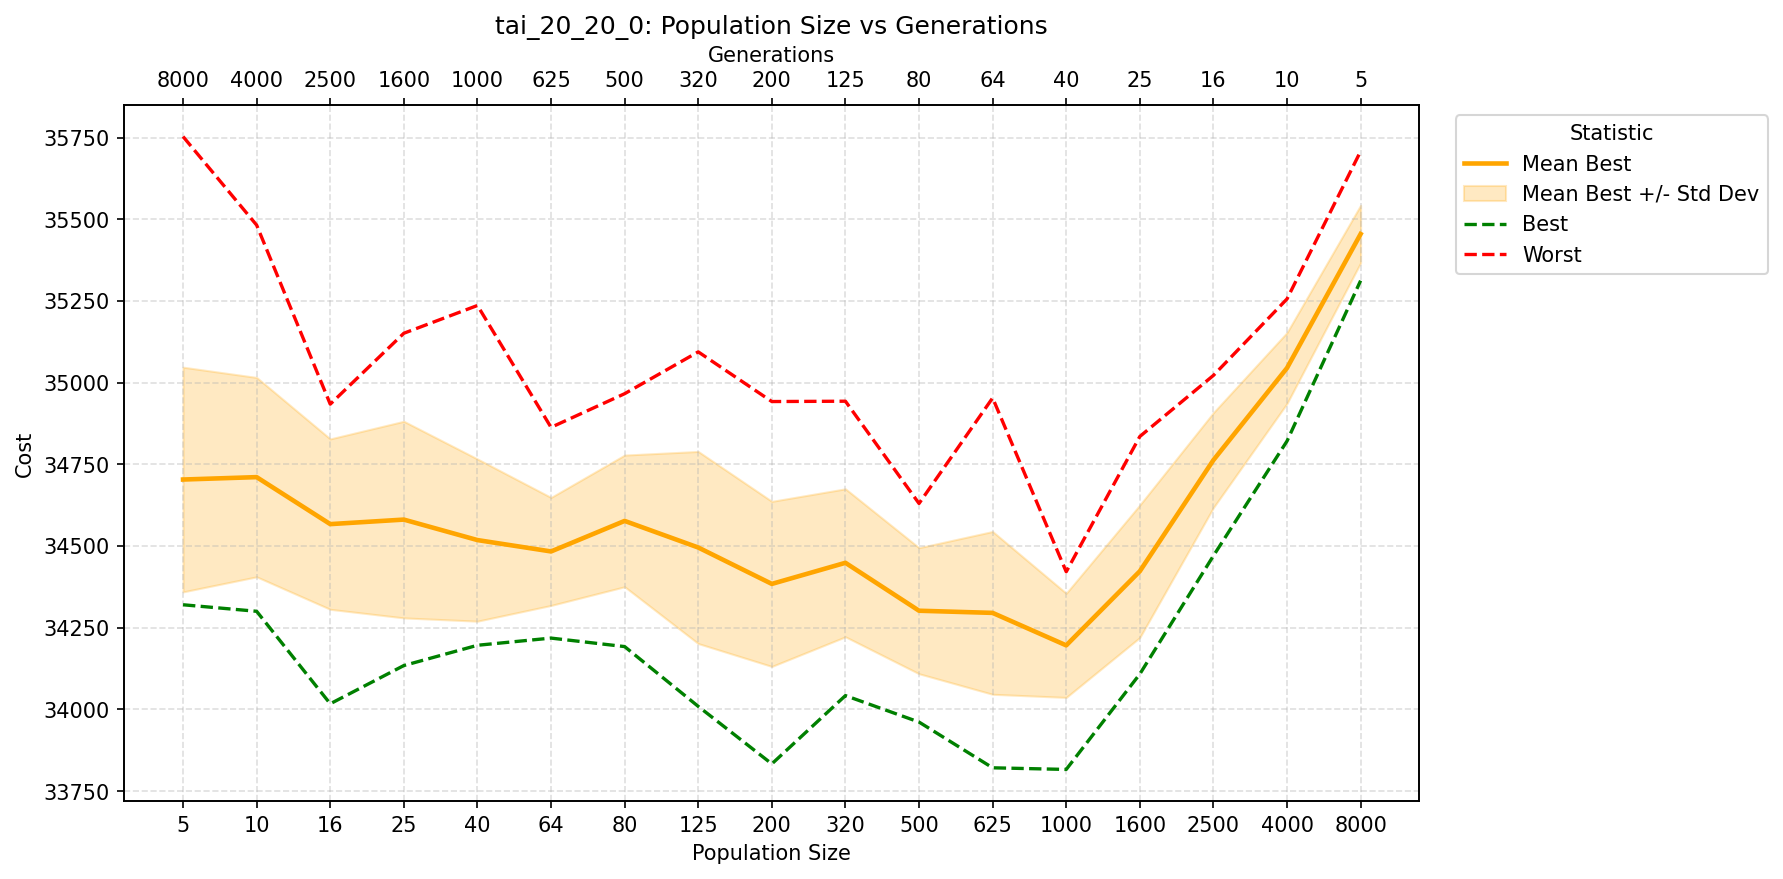
\includegraphics[width=0.48\textwidth]{../Experiments/01_default_evolutionary_population_generations/fig_tai_20_20_0.png}
\hfill
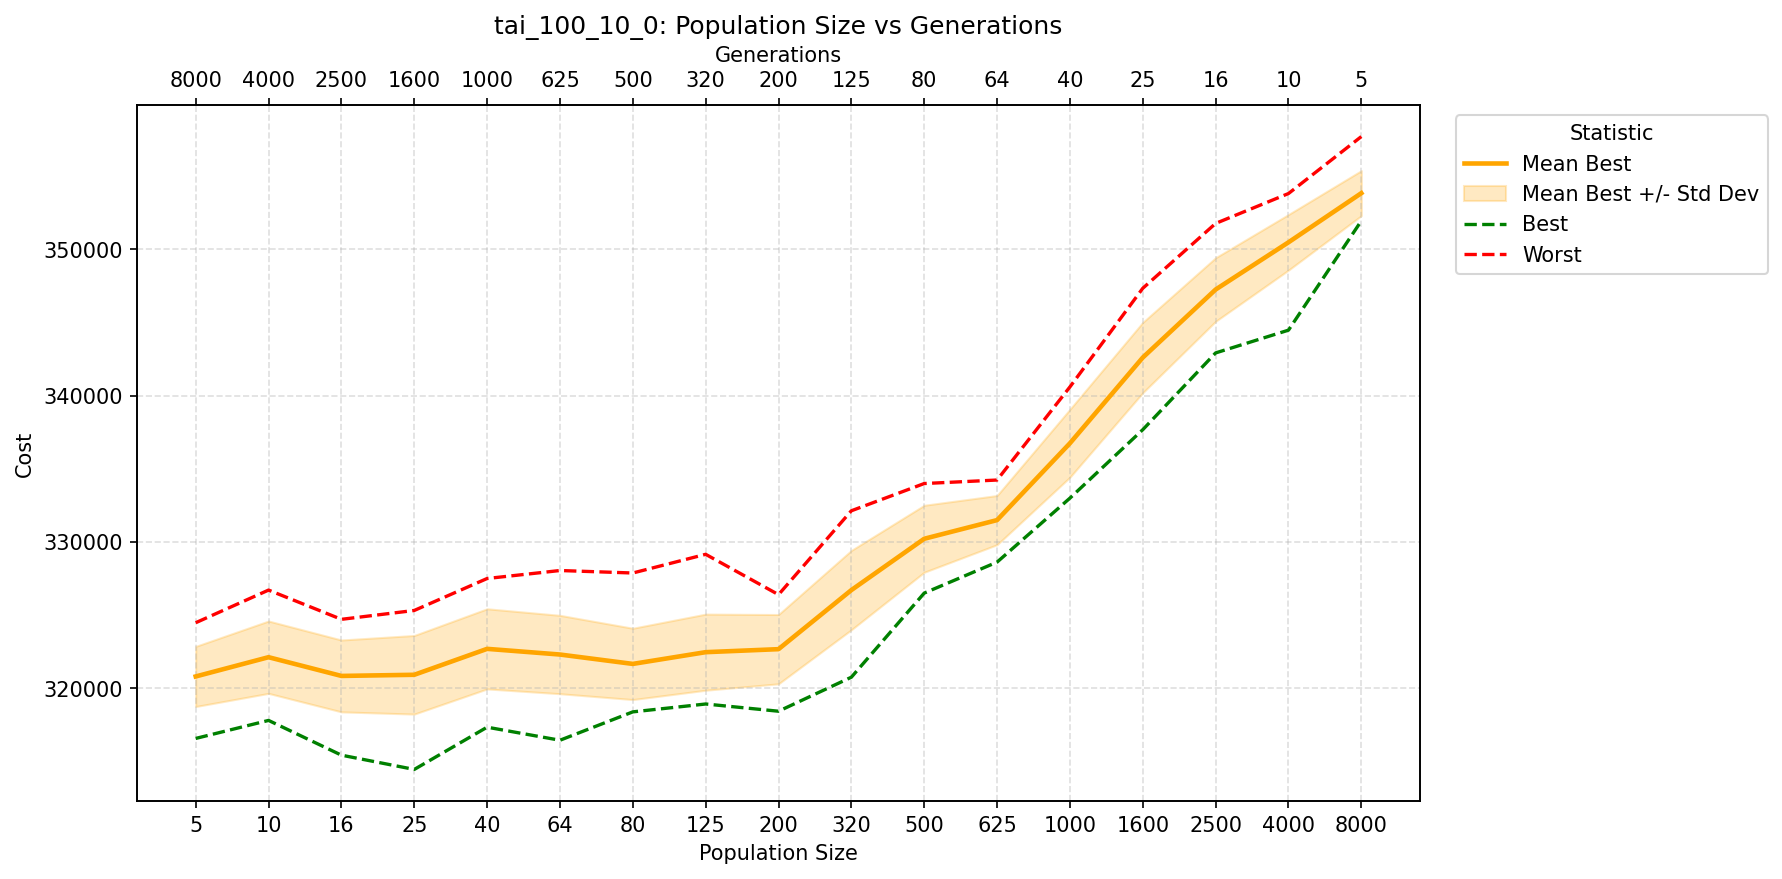
\includegraphics[width=0.48\textwidth]{../Experiments/01_default_evolutionary_population_generations/fig_tai_100_10_0.png}

\vspace{0.5em}

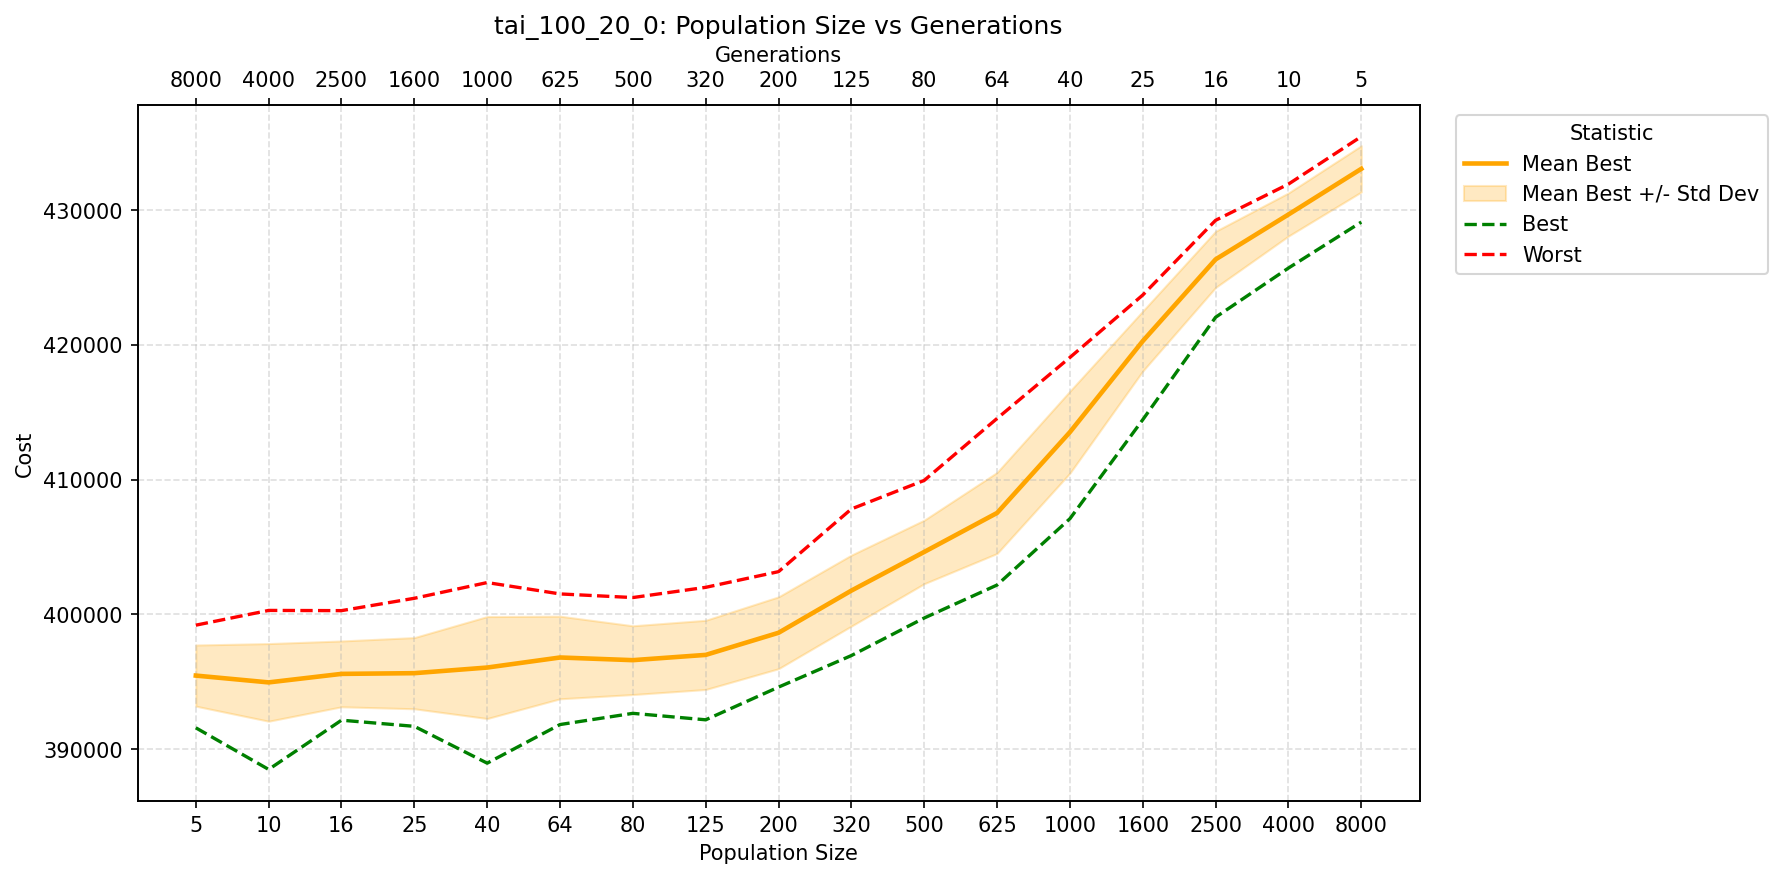
\includegraphics[width=0.48\textwidth]{../Experiments/01_default_evolutionary_population_generations/fig_tai_100_20_0.png}
\hfill
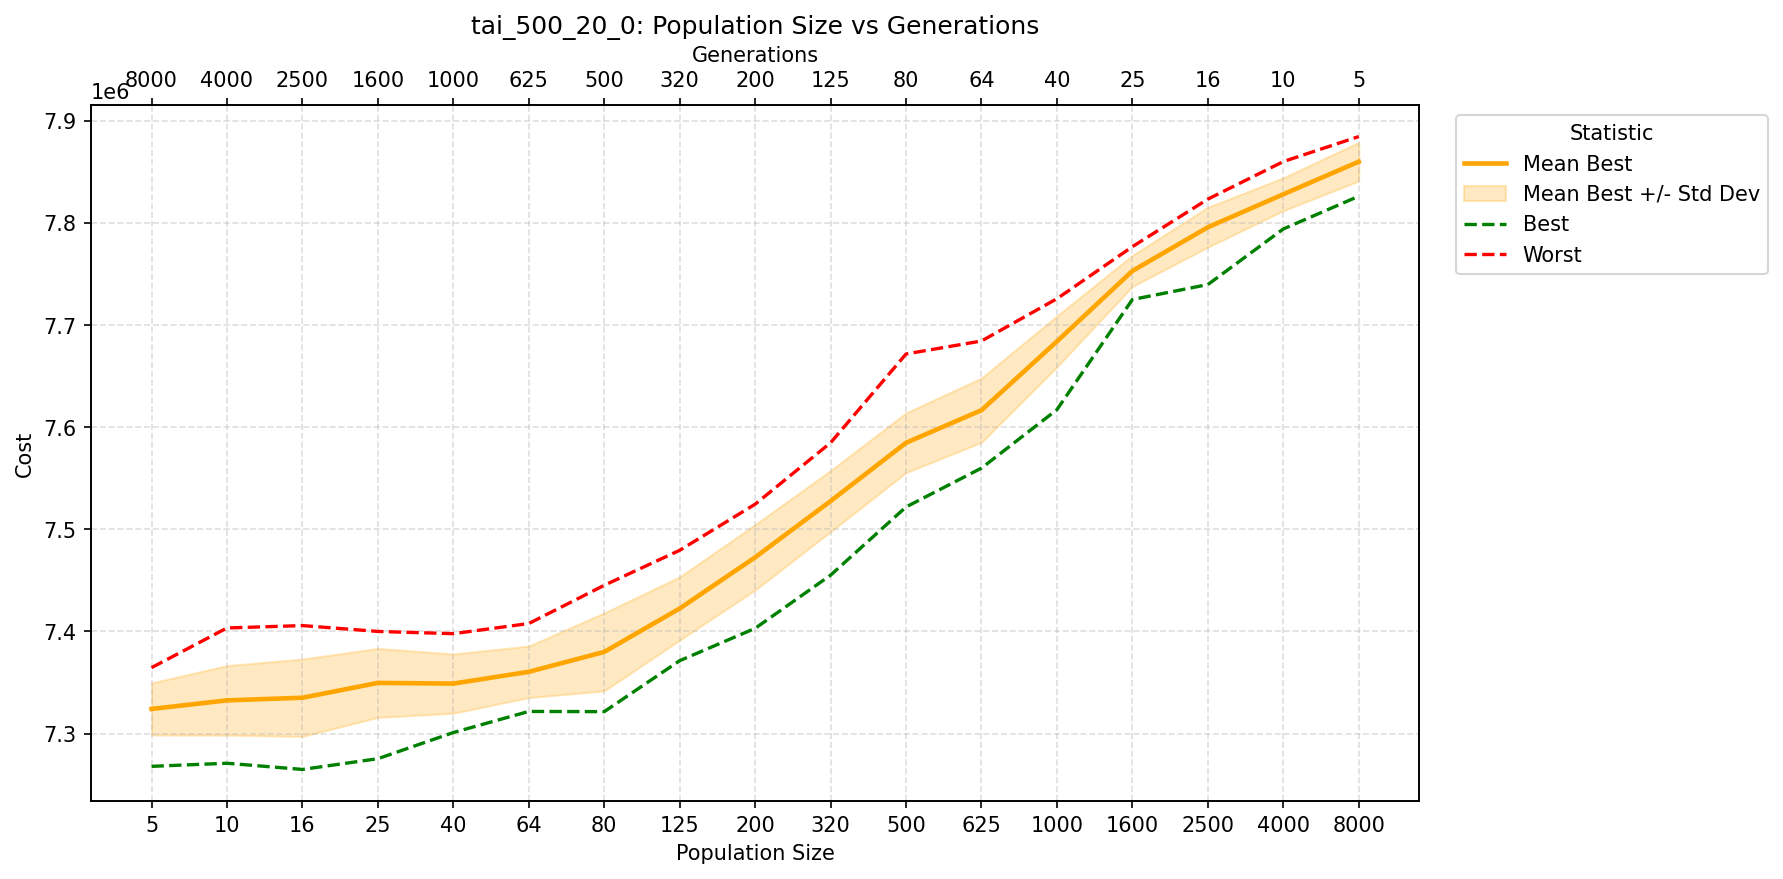
\includegraphics[width=0.48\textwidth]{../Experiments/01_default_evolutionary_population_generations/fig_tai_500_20_0.png}
\caption{Population size vs. generations surfaces for default Taillard instances (EA pilot).}
\label{fig:ea_pop_gen_surfaces_tai}
\end{figure}

\subsubsection*{Population size vs Generations Aggregated Analysis (Best Cost by NFE)}
The number of fitness evaluations (NFE) is used to aggregate results, collapsing the grid to a one-dimensional axis, giving a more general view of the relationship between search effort and solution quality.


\begin{figure}[H]
\centering
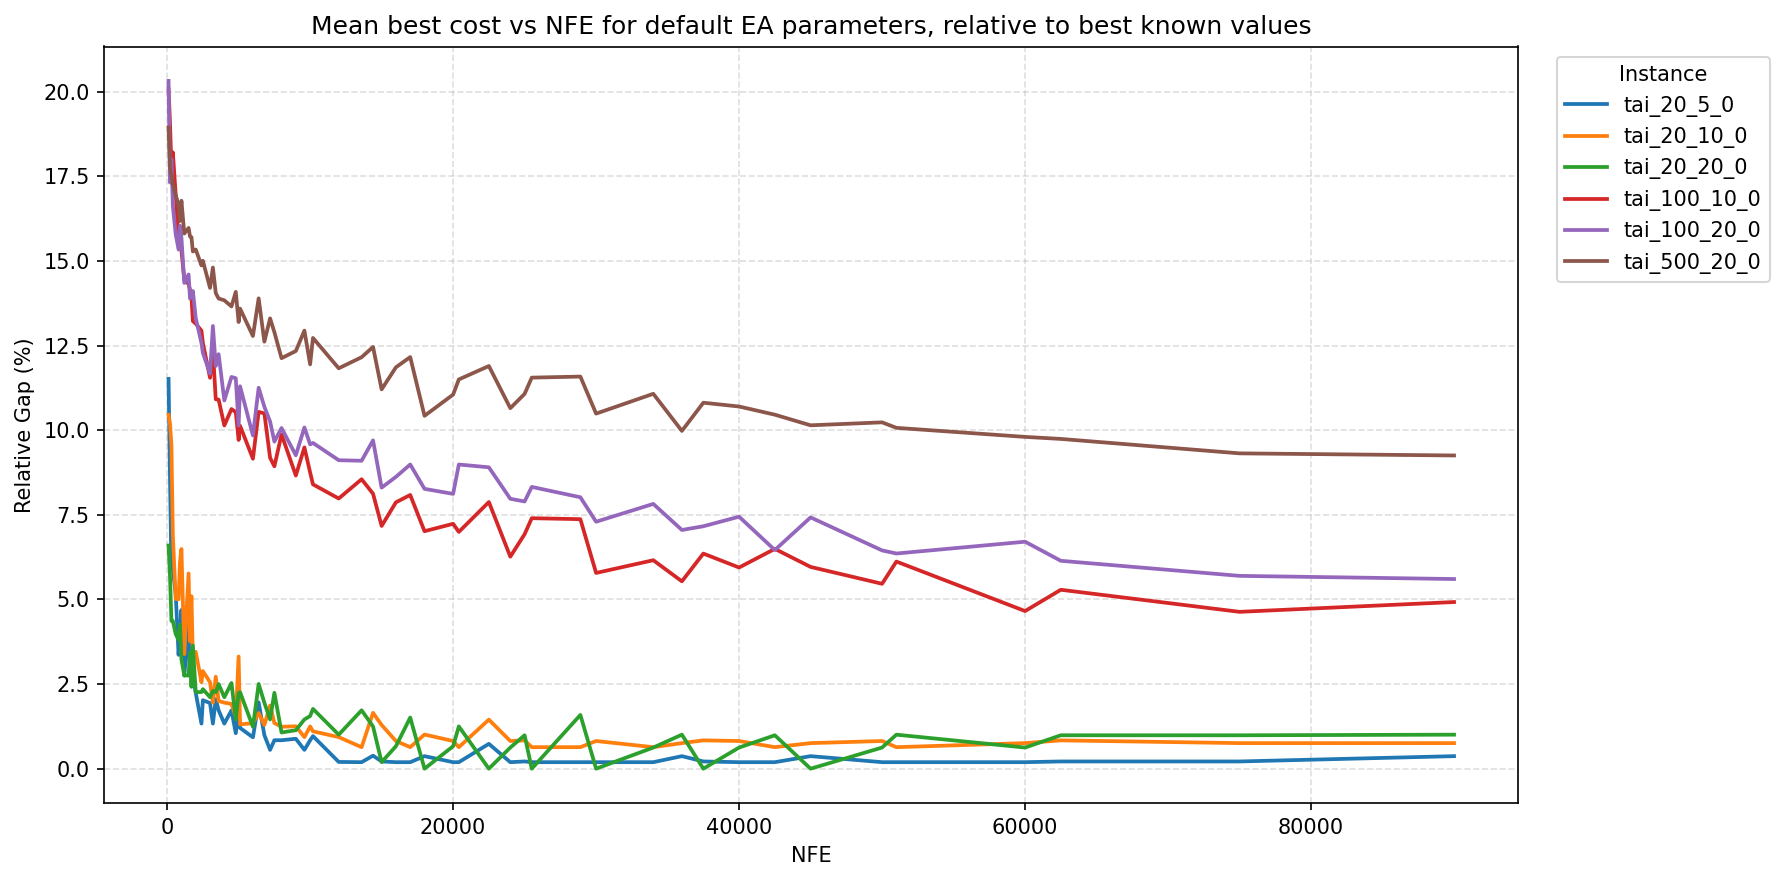
\includegraphics[width=0.48\textwidth]{../Experiments/01_default_evolutionary_population_generations/fig_all_aggregate.png}

\vspace{0.5em}
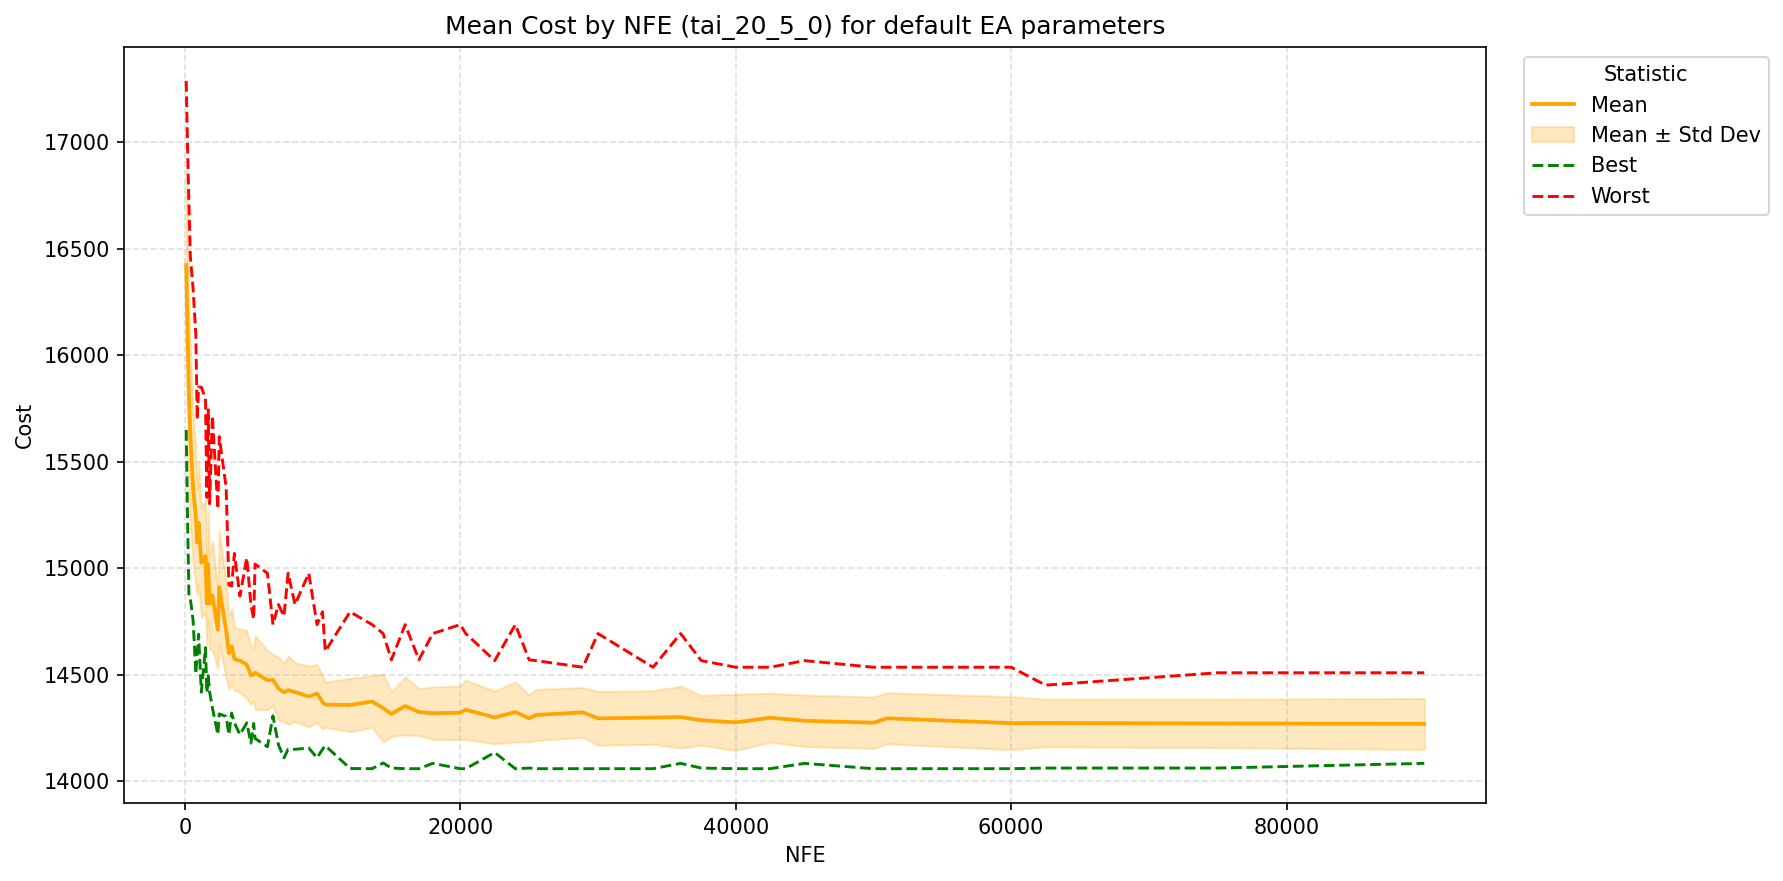
\includegraphics[width=0.48\textwidth]{../Experiments/01_default_evolutionary_population_generations/fig_tai_20_5_0_aggregate.png}
\hfill
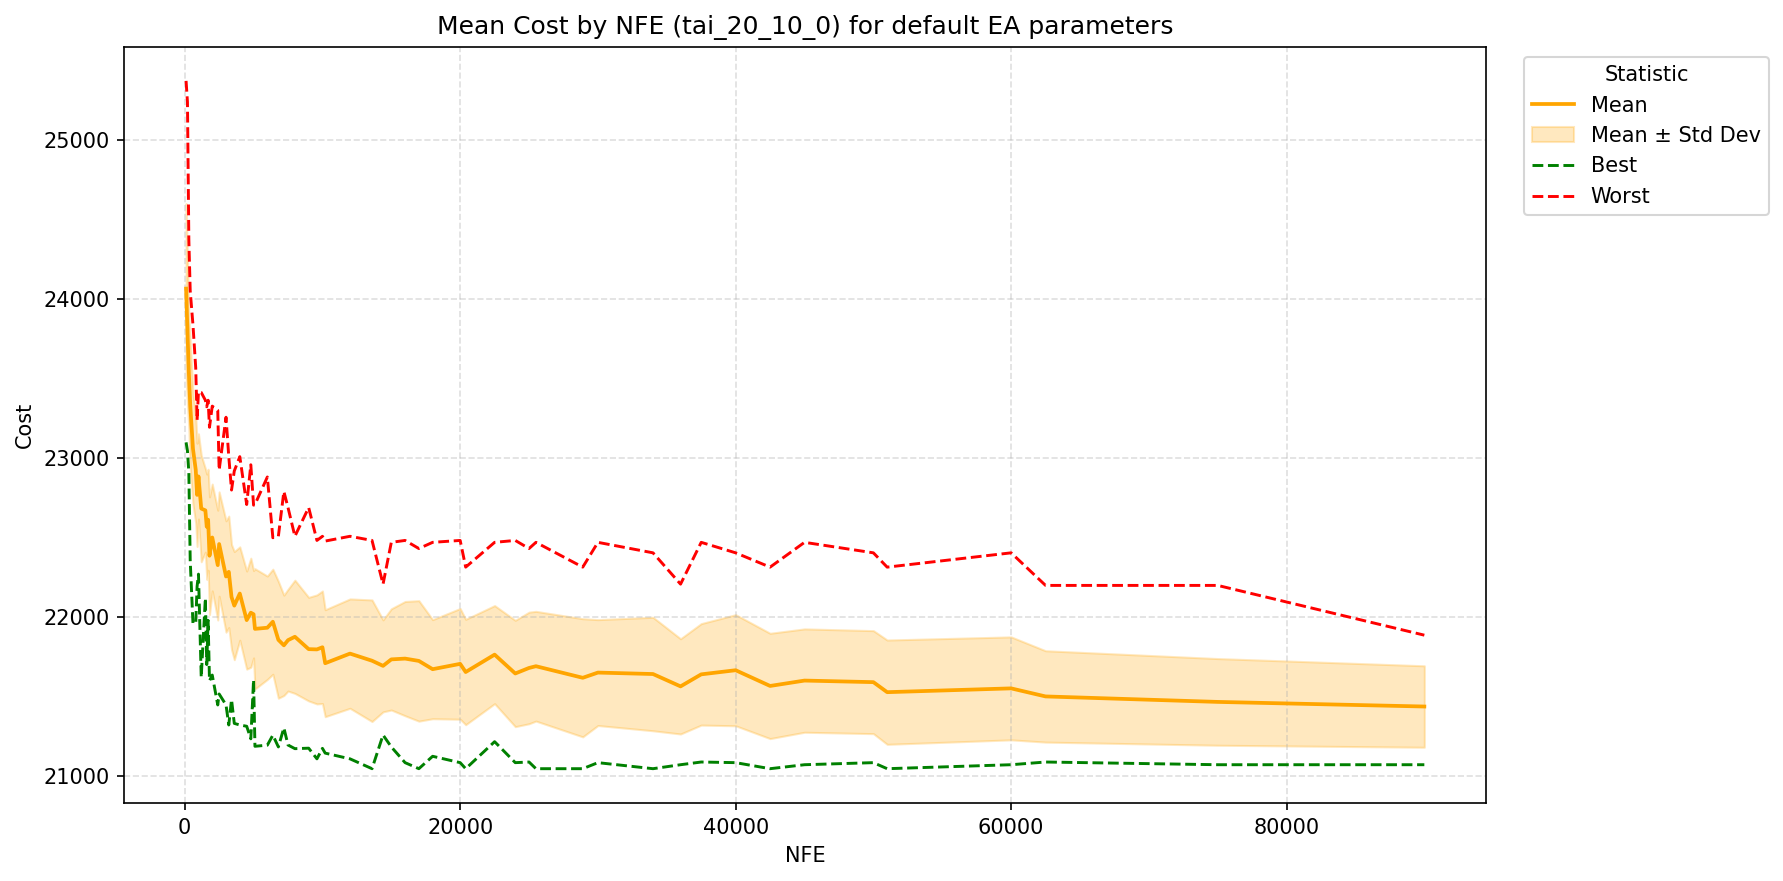
\includegraphics[width=0.48\textwidth]{../Experiments/01_default_evolutionary_population_generations/fig_tai_20_10_0_aggregate.png}

\vspace{0.5em}

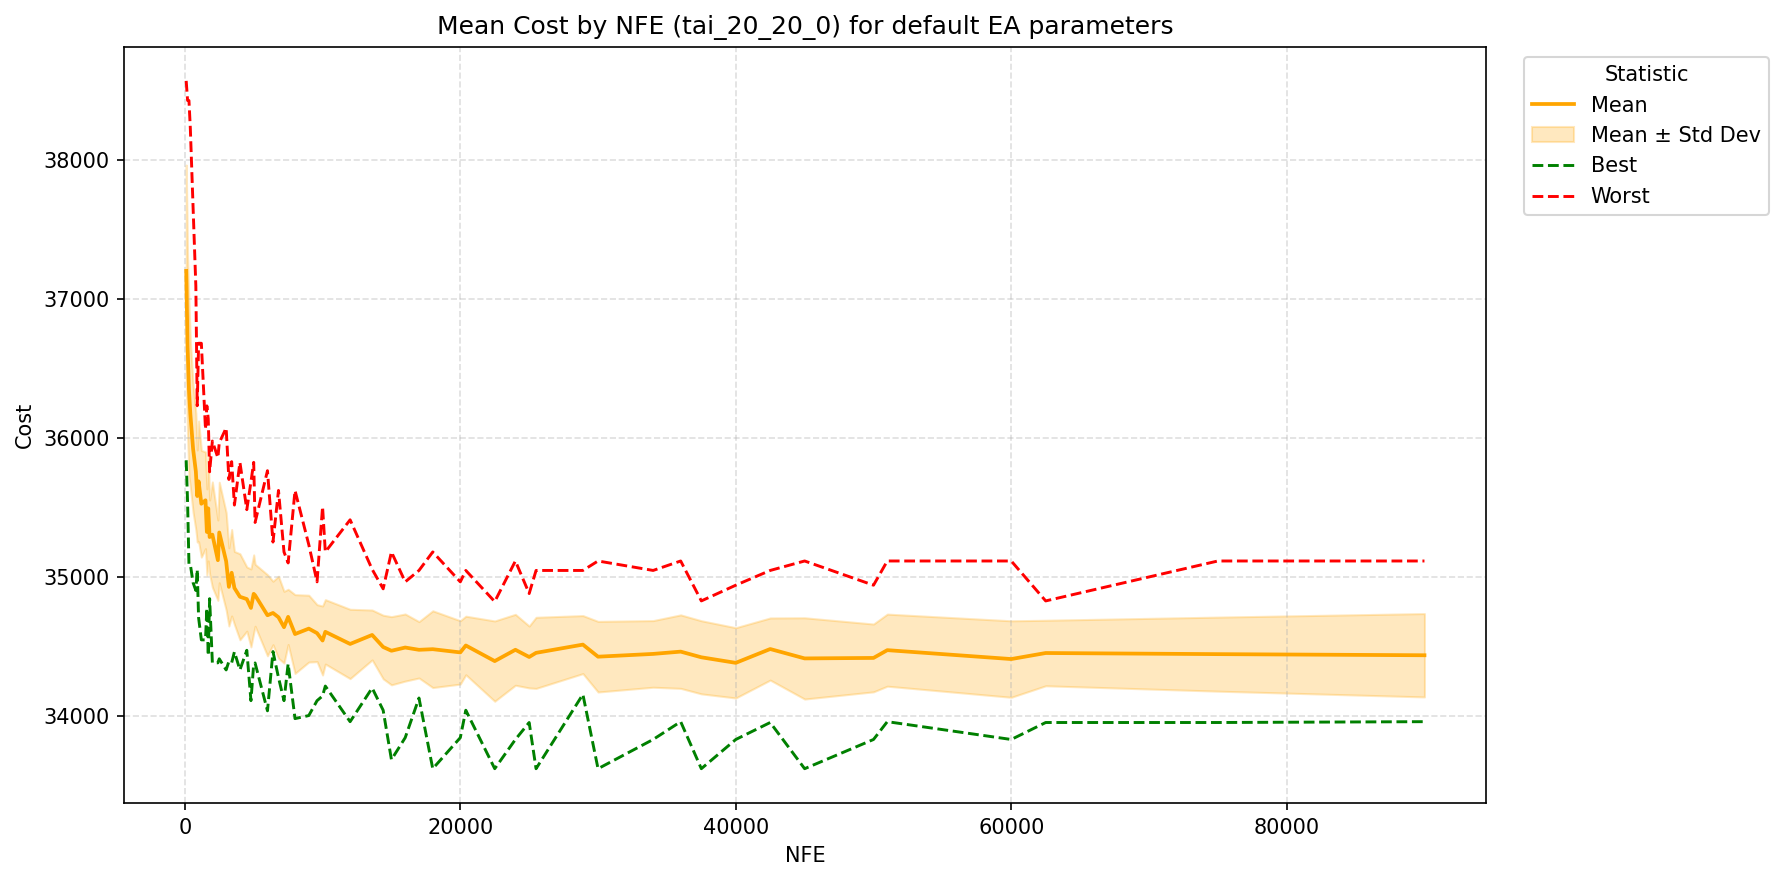
\includegraphics[width=0.48\textwidth]{../Experiments/01_default_evolutionary_population_generations/fig_tai_20_20_0_aggregate.png}
\hfill
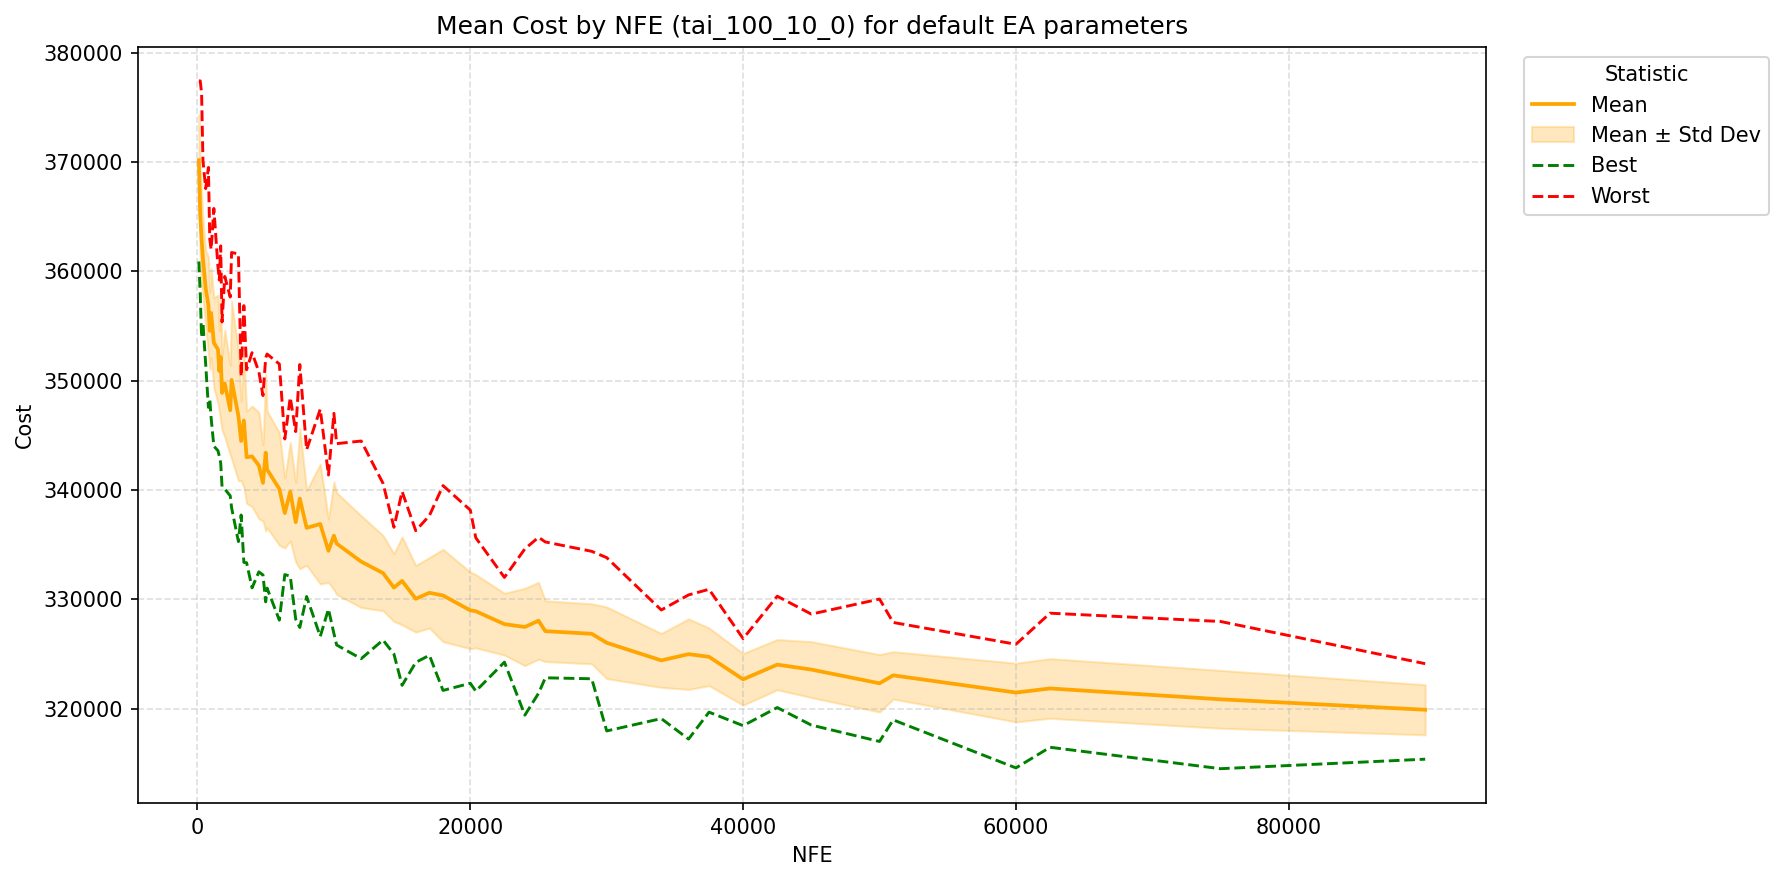
\includegraphics[width=0.48\textwidth]{../Experiments/01_default_evolutionary_population_generations/fig_tai_100_10_0_aggregate.png}

\vspace{0.5em}

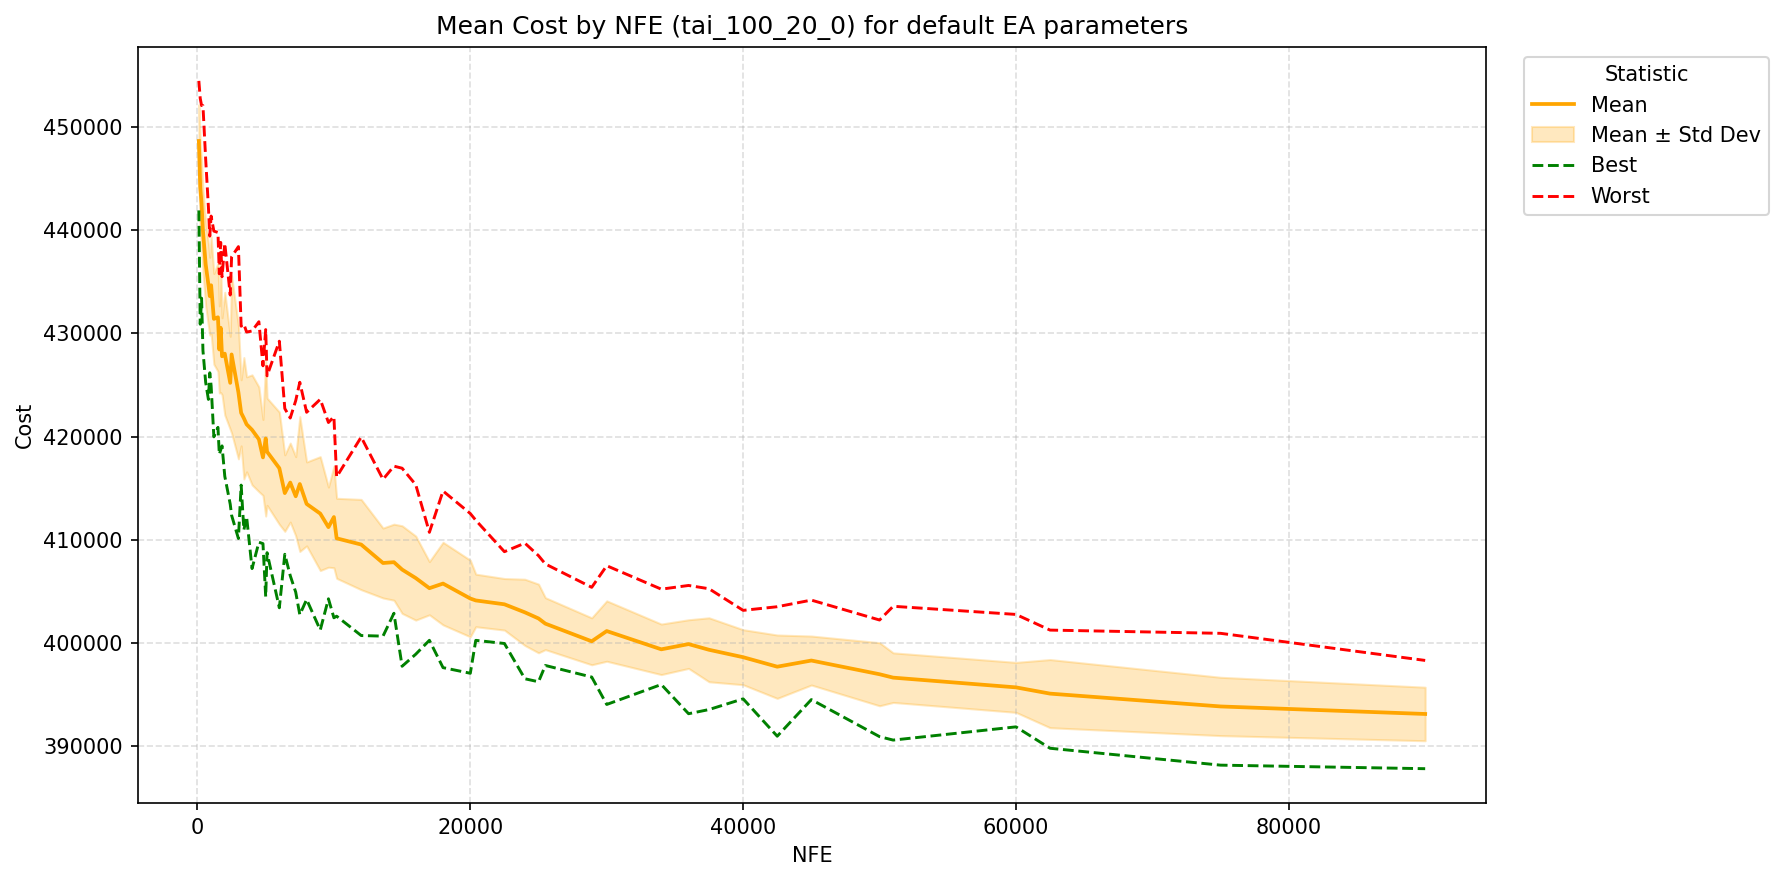
\includegraphics[width=0.48\textwidth]{../Experiments/01_default_evolutionary_population_generations/fig_tai_100_20_0_aggregate.png}
\hfill
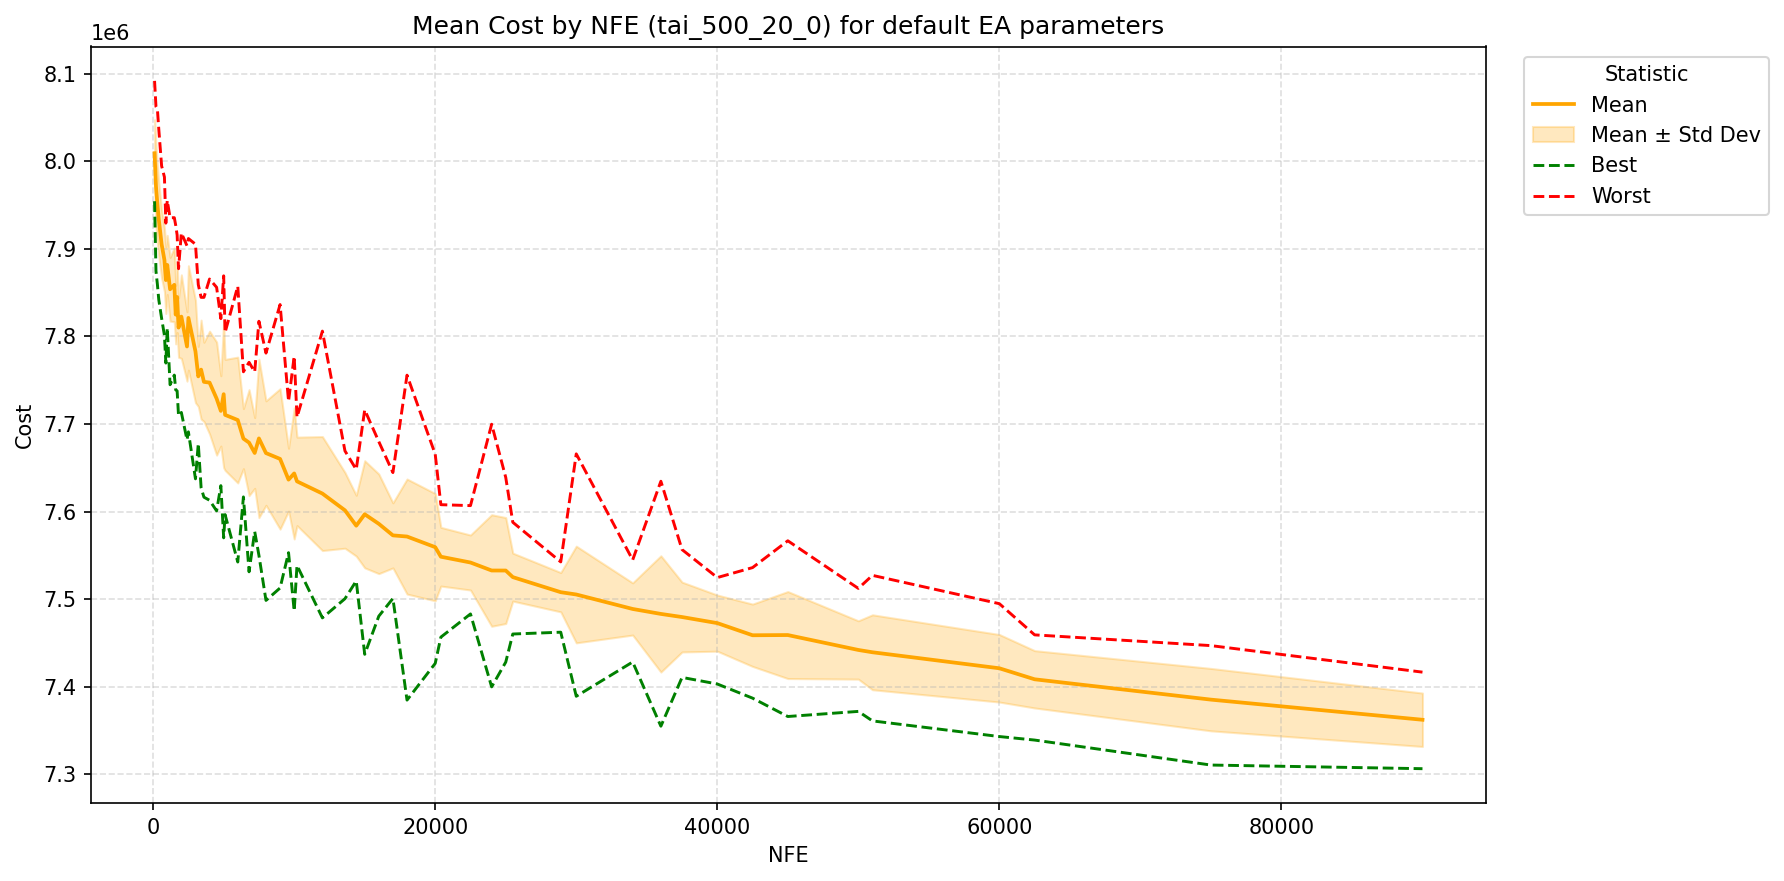
\includegraphics[width=0.48\textwidth]{../Experiments/01_default_evolutionary_population_generations/fig_tai_500_20_0_aggregate.png}
\caption{Population size vs. generations surfaces for default Taillard instances (EA pilot).}
\label{fig:ea_pop_gen_surfaces_tai_aggregated}
\end{figure}

\subsubsection*{Final Budget Selection}
Based on the above analyses, a budget of \(B = 40{,}000\) evaluations is selected for the main study.


\chapter{Compared Optimization Methods}
\section{Random Search}
Random Search is the stochastic baseline. It samples random permutations, evaluates them, and keeps the best found.

The implementation supports sequential and parallel sampling. Final experiments use the sequential setup.

Stopping can use an evaluation budget or a time limit. In this study, an evaluation budget is used.

\section{Greedy Heuristic}
Two deterministic constructive baselines are used:

\paragraph{Greedy}
Greedy sorts jobs by total processing time (ascending) and returns that permutation.

\paragraph{SPT (NEH-like iterative greedy).}
SPT starts from the same priority order but inserts each next job at the best position in the current partial sequence (NEH-like constructive strategy).

Both return one final permutation and serve as low-cost references.

\section{Evolutionary Algorithm (EA)}
EA is a population-based stochastic search. It iterates selection, crossover, mutation, and full generational replacement.

Default configuration used when not otherwise specified:
\begin{itemize}
    \item Population size: $100$
    \item Generations: $100$
    \item Crossover rate: $0.7$
    \item Mutation rate: $0.1$
    \item Tournament size: $5$
    \item Selection method: Tournament
    \item Crossover operator: OX (Order Crossover)
    \item Mutation operator: Swap
\end{itemize}

Implemented operators: mutation (Swap, Insert), crossover (Order Crossover OX, Cycle Crossover CX), selection (Tournament).

\section{Simulated Annealing (SA)}
Simulated Annealing is a neighborhood local search with temperature-based acceptance.

In this study, SA parameters are fixed (no tuning) and used as a stable baseline.
Default configuration used in the experiment runner:
\begin{itemize}
    \item Iterations: $10{,}000$
    \item Initial temperature: $T_0 = 100.0$
    \item Cooling rate: $\alpha = 0.995$ (not used in linear schedule)
    \item Minimum temperature: $T_{\min} = 10^{-4}$
    \item Neighborhood operator: Swap
    \item Acceptance function: Probabilistic (Metropolis-type)
    \item Cooling schedule: Linear
\end{itemize}

With the default linear cooling schedule, temperature is updated as
\[
T_{k+1} = 1 - \frac{k}{K},
\]
where $k$ is the current iteration index (starting from $0$ in this form) and $K$ is the maximum number of iterations. In the current implementation, the linear schedule does not use $\alpha$ directly.

For the default probabilistic acceptance function, let $f(x)$ be the current solution cost and $f(x')$ the candidate cost. Acceptance is defined by
\[
P(\text{accept } x'\mid x, T)=
\begin{cases}
1, & f(x') \le f(x),\\
\exp\!\left(-\dfrac{f(x')-f(x)}{T}\right), & f(x') > f(x).
\end{cases}
\]
Improving moves are always accepted. Worsening moves are accepted with probability that decreases with temperature.


\chapter{Baseline Results}
\section{Baseline Experiment Design}
This baseline experiment compares all algorithms with their default parameters on the same six benchmark instances. Each algorithm uses a maximum computational budget of 40\,000 fitness evaluations per run. Results report the mean final cost over \textbf{n = 20} independent runs for each algorithm–instance combination.

\section{Baseline Results by Instance}
The plots and tables below present per-instance baseline results, showing how each algorithm performs across problem sizes and complexity.


\begin{figure}[H]
\centering
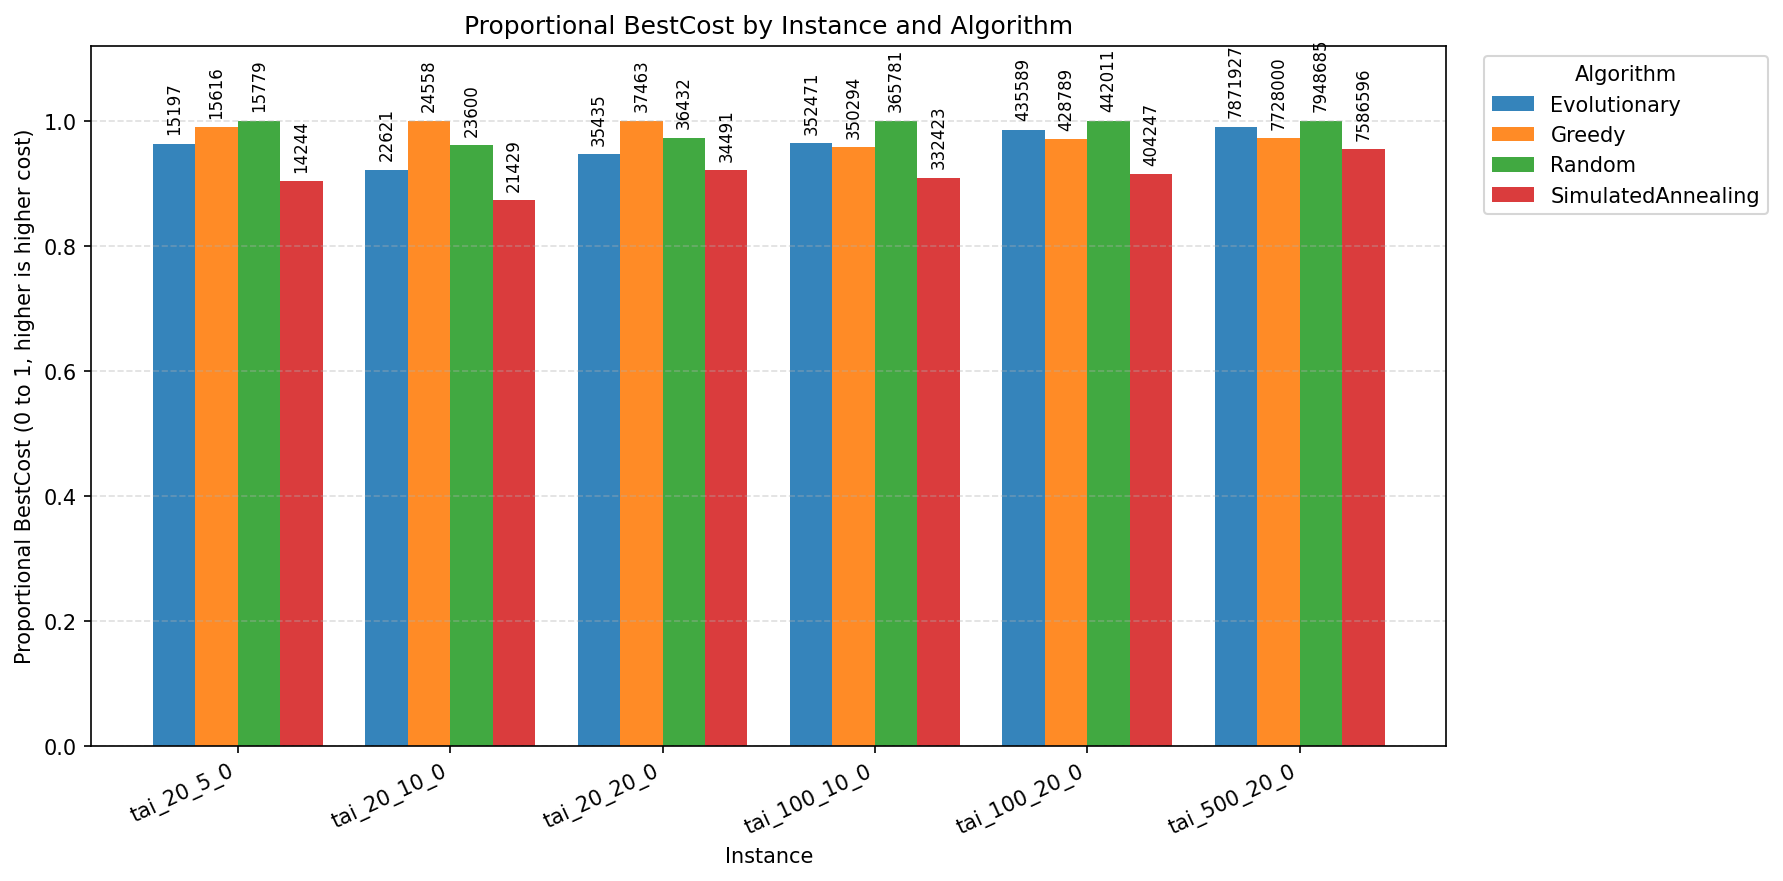
\includegraphics[width=0.9\textwidth]{../Experiments/03_default_all_algorithms/all_default.png}
\caption{Baseline comparison of all methods on all instances.}
\label{fig:baseline_all_aggregate}
\end{figure}

\paragraph{Baseline comparison table.}
The following table is loaded from \texttt{data.csv} and scaled to page width.

\begin{table}[H]
\centering
\resizebox{\textwidth}{!}{%
\csvautotabular{data.csv}
}
\end{table}

\chapter{Evolutionary Algorithm Design Details}
\section{Encoding and Initialization}
Each EA individual is a permutation of job indices (a valid schedule).

\paragraph{Permutation Representation.}
Let $J$ denote the number of jobs. An individual is encoded as a vector $x = (x_1, x_2, \ldots, x_J)$, where $x_j$ is the index of the job assigned to position $j$ in the sequence. The set of all possible individuals is the set of all permutations of $\{1, \ldots, J\}$.

\paragraph{Initial Population Generation.}
The initial population is $P$ random permutations generated with seeded randomness for reproducibility.

\section{Fitness Evaluation}
The evaluator computes Total Flow Time using a dynamic-programming recurrence over the machine dimension and the position in the permutation.
For a fixed permutation prefix, the state stores completion times propagated across machines.

Implementation-wise, this is realized in \texttt{PFSP.Evaluators.TotalFlowTimeEvaluator.Evaluate} with a one-dimensional buffer
(\texttt{comp}) representing the completion frontier for the current machine pass. For each machine, the evaluator performs a left-to-right scan over jobs in the permutation and updates:
\[
C_{m,p} = p_{m,\pi_p} + \max(C_{m-1,p}, C_{m,p-1}),
\]
with boundary handling for \(m=0\) and \(p=0\).

This DP formulation keeps the algorithm at \(\mathcal{O}(M\cdot N)\) per evaluation (for \(M\) machines and \(N\) assigned jobs),
while using \(\mathcal{O}(N)\) temporary memory via the reusable completion buffer.

\section{Selection, Crossover, Mutation, Replacement}
The EA uses standard permutation operators:

\paragraph{Selection.}
Tournament selection samples a subset and picks the best individual. Tournament size controls selection pressure.

\paragraph{Crossover.}
Two crossover operators are implemented:
\begin{itemize}
    \item \textbf{Order Crossover (OX):} This operator creates offspring by copying a contiguous segment from one parent and filling the remaining positions with the order of jobs from the other parent, skipping duplicates. OX preserves relative job order and is well-suited for permutation problems.
    \item \textbf{Cycle Crossover (CX):} This operator identifies cycles between two parents and exchanges them to produce offspring, ensuring that each job appears exactly once. CX maintains absolute position inheritance from both parents.
\end{itemize}
Crossover method and probability are configurable.

\paragraph{Mutation.}
Two mutation operators are available:
\begin{itemize}
    \item \textbf{Swap Mutation:} Two positions in the permutation are selected at random, and their jobs are swapped. This is a simple and effective way to introduce local diversity.
    \item \textbf{Insert Mutation:} A job is removed from one position and inserted at another, shifting the intermediate jobs. This operator can produce larger changes in the permutation structure.
\end{itemize}
Mutation method and probability are configurable.

\paragraph{Replacement.}
Replacement is full generational. Elitism is handled separately.

\section{Elitism and Termination}
Elitism and termination are explicit in the implementation.

\paragraph{Elitism.}
\texttt{ElitismK} controls how many top individuals are copied unchanged to the next generation. If \texttt{ElitismK}=0, there is no elitism.

\paragraph{Termination.}
Termination uses \texttt{Generations}, optionally capped by \texttt{EvaluationBudget}. The algorithm always reports the best solution found.

\chapter{EA Parameter Sensitivity Analysis}
\section{Single-Parameter Screening}
One-factor-at-a-time (OFAT) screening is used: one EA parameter is varied while others are kept at default values. The Population and Generation

The following parameters were screened:
\begin{itemize}
    \item \textbf{Mutation probability} ($p_{mut}$)
    \item \textbf{Crossover probability} ($p_{cross}$)
    \item \textbf{Tournament size} ($k_{tour}$): Corresponds to selection pressure.
    \item \textbf{Population size and Generation count} ($P$ and $G$) are analyzed together in a paired sweep to understand their interaction under a fixed evaluation budget.
\end{itemize}

For each setting, EA runs on all benchmark instances under the same evaluation budget as the main study. Each configuration uses $n=20$ independent seeds.

Primary metric: best TFT per run. Mean and standard deviation by parameter value are reported against the default.

\section{Population Size and Generation Count}

In this analysis, population size and generation count are treated as a bound pair under a fixed computational budget. For each tested setting, one axis is used to show population size and a second axis is used to show the tied generation value. This two-axis presentation is used because each plotted point corresponds to one paired \((P,G)\).

\begin{figure}[H]
\centering
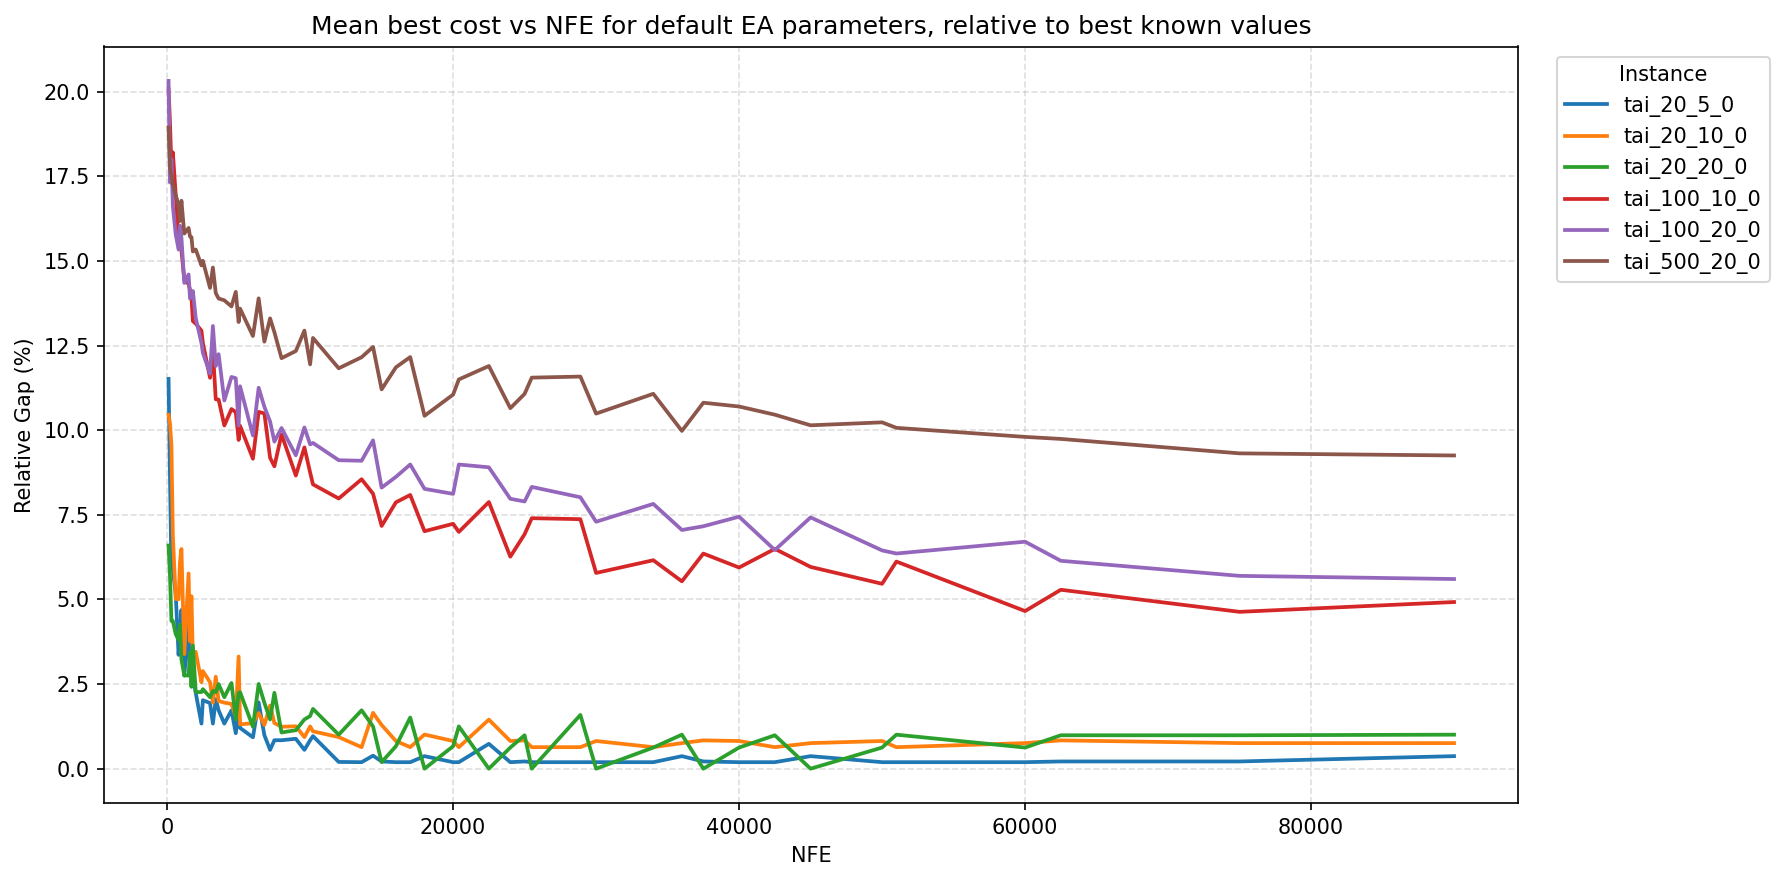
\includegraphics[width=0.48\textwidth]{../Experiments/01_default_evolutionary_population_generations/fig_all_aggregate.png}

\vspace{0.5em}
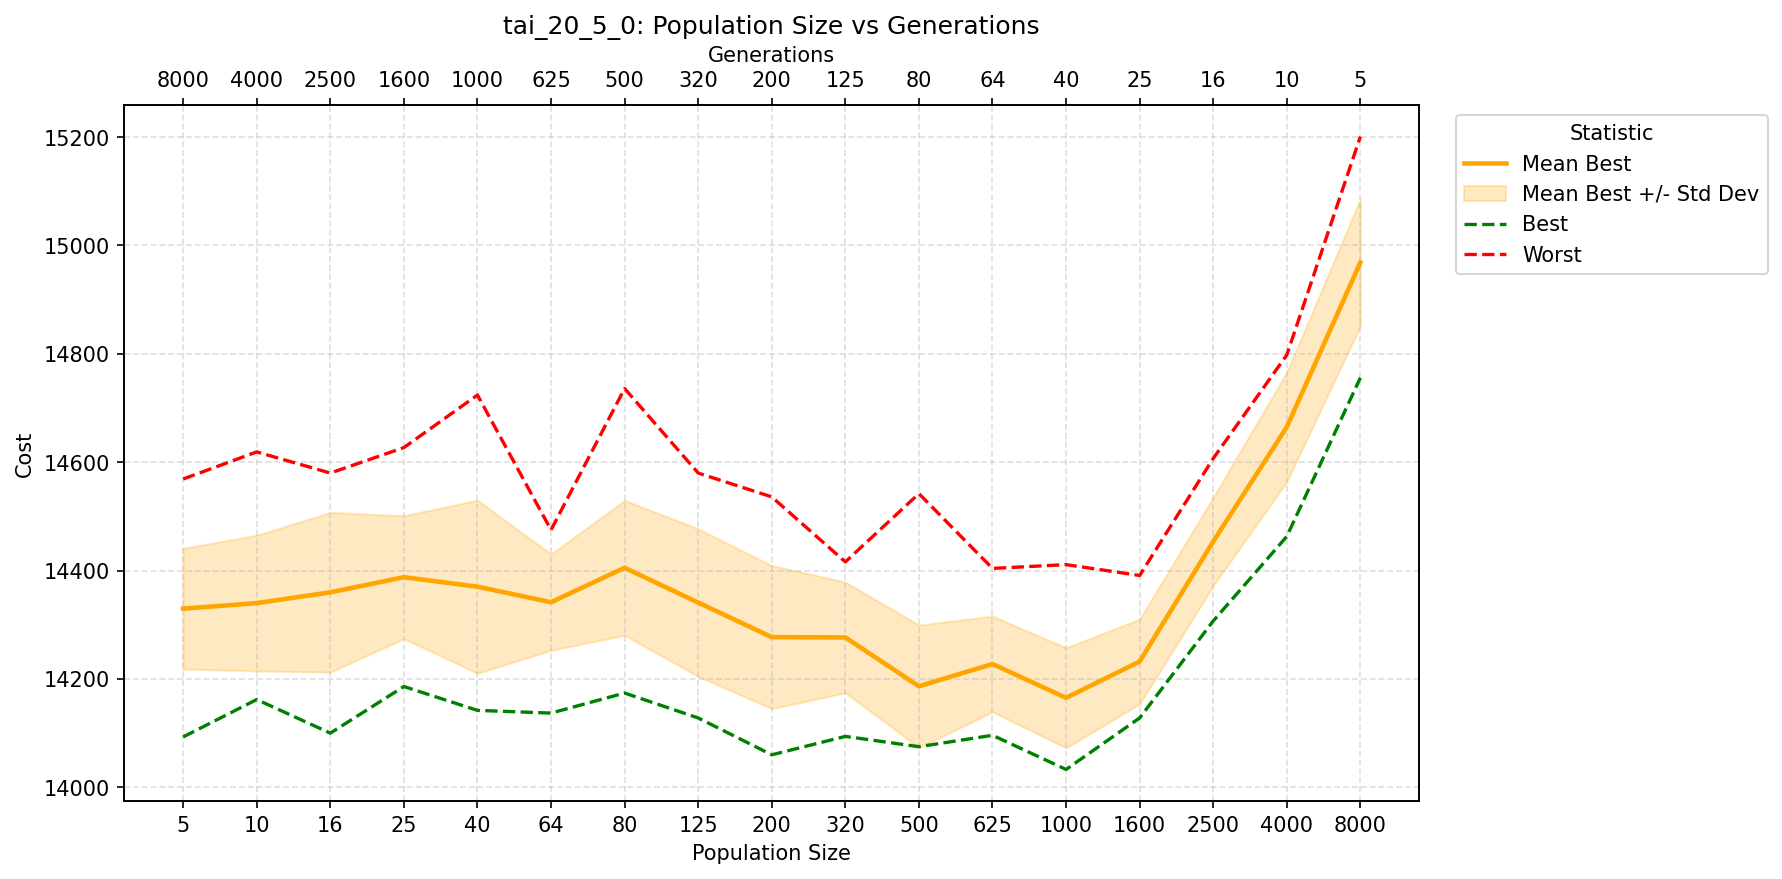
\includegraphics[width=0.48\textwidth]{../Experiments/01_default_evolutionary_population_generations/fig_tai_20_5_0_pair.png}
\hfill
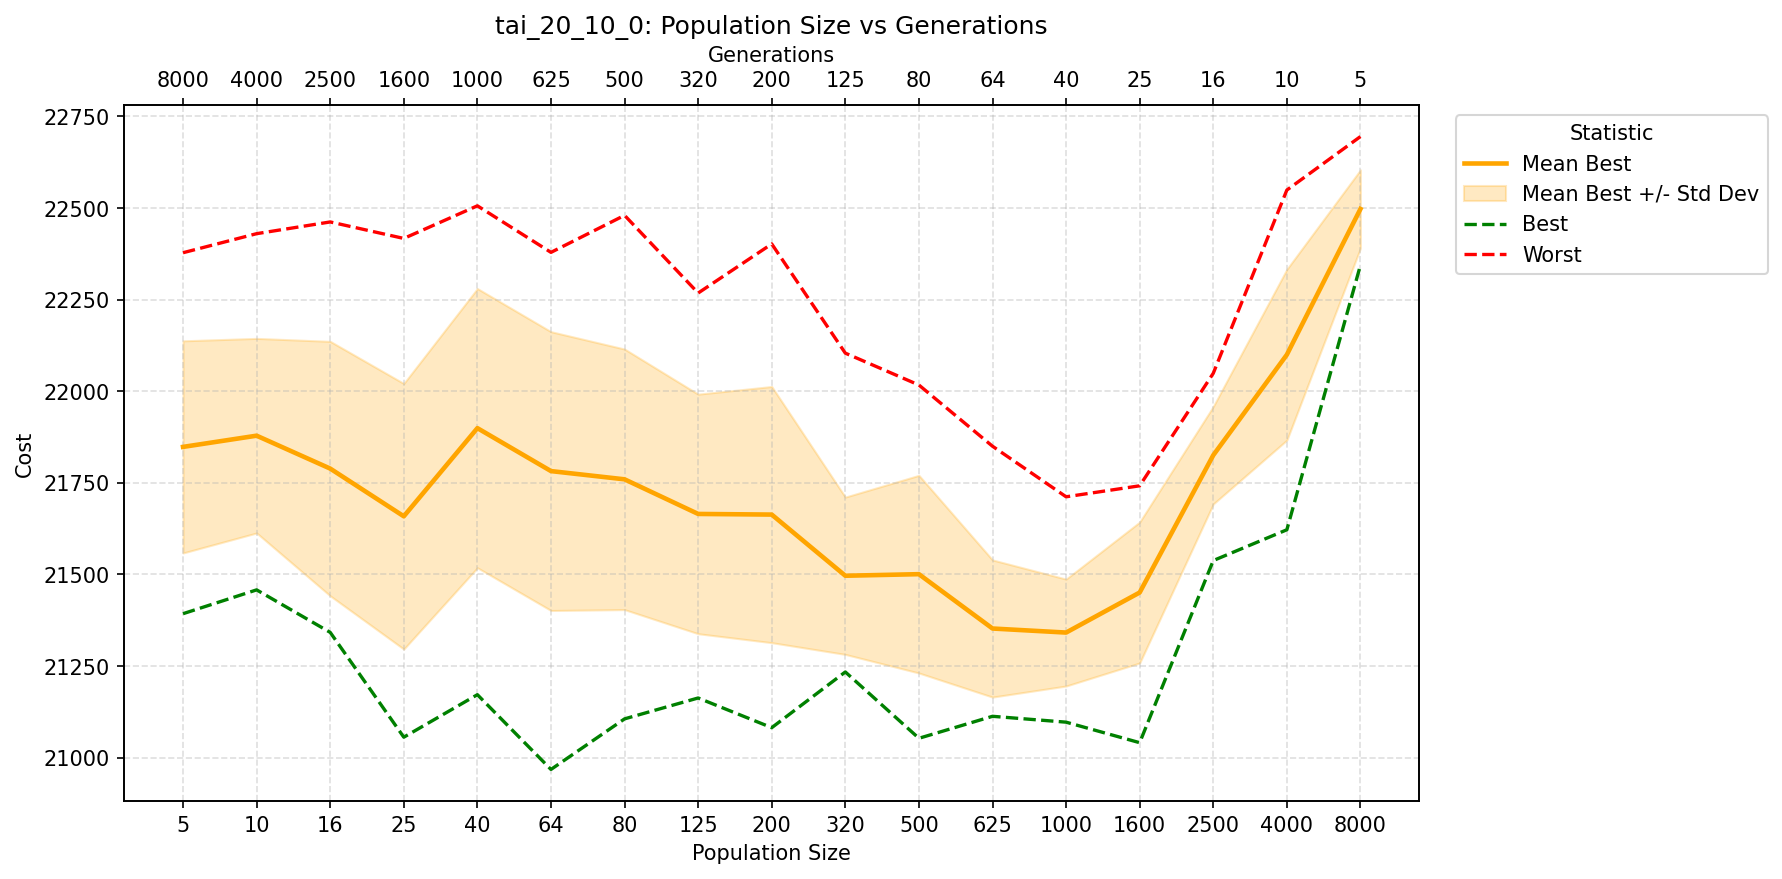
\includegraphics[width=0.48\textwidth]{../Experiments/01_default_evolutionary_population_generations/fig_tai_20_10_0_pair.png}

\vspace{0.5em}

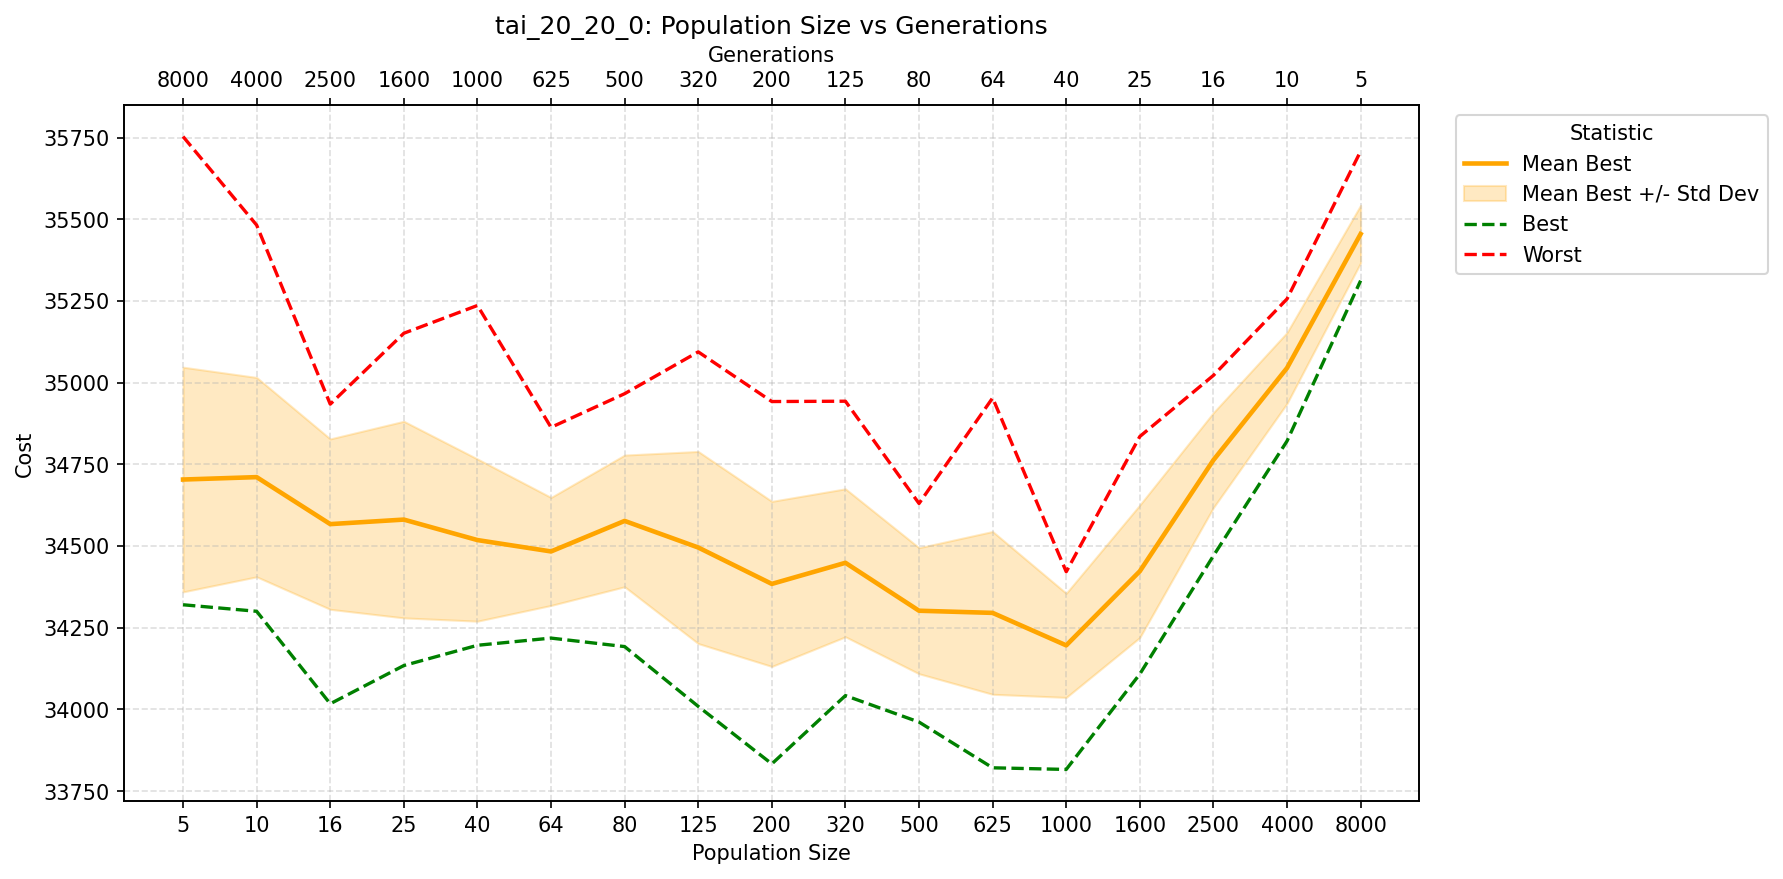
\includegraphics[width=0.48\textwidth]{../Experiments/01_default_evolutionary_population_generations/fig_tai_20_20_0_pair.png}
\hfill
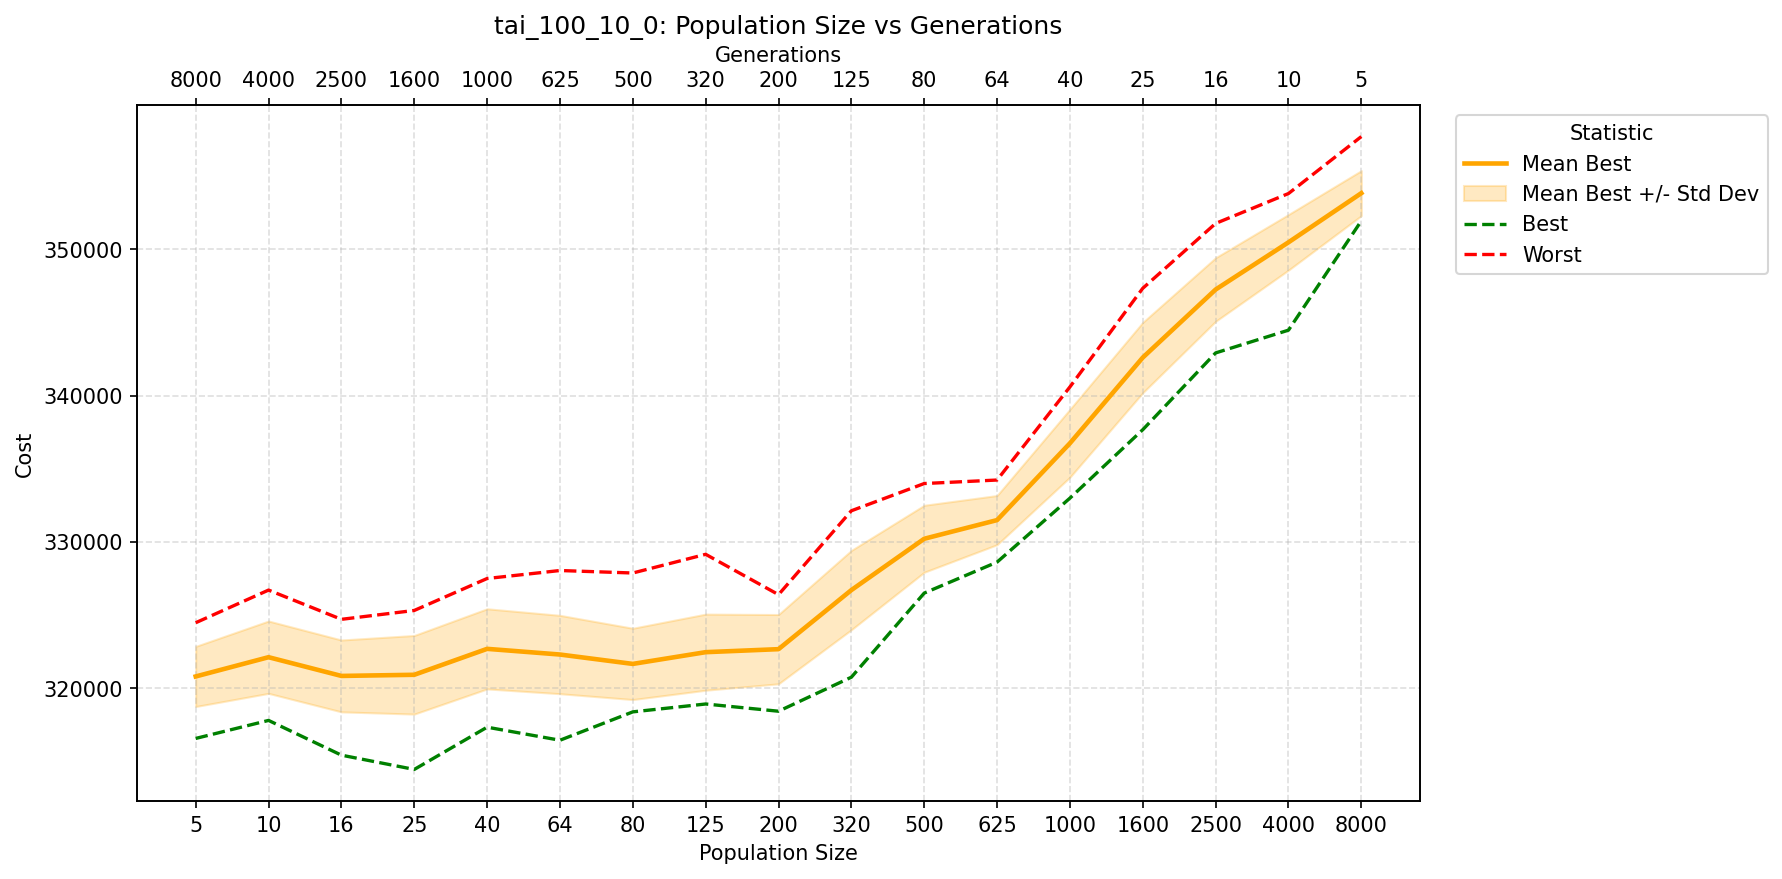
\includegraphics[width=0.48\textwidth]{../Experiments/01_default_evolutionary_population_generations/fig_tai_100_10_0_pair.png}

\vspace{0.5em}

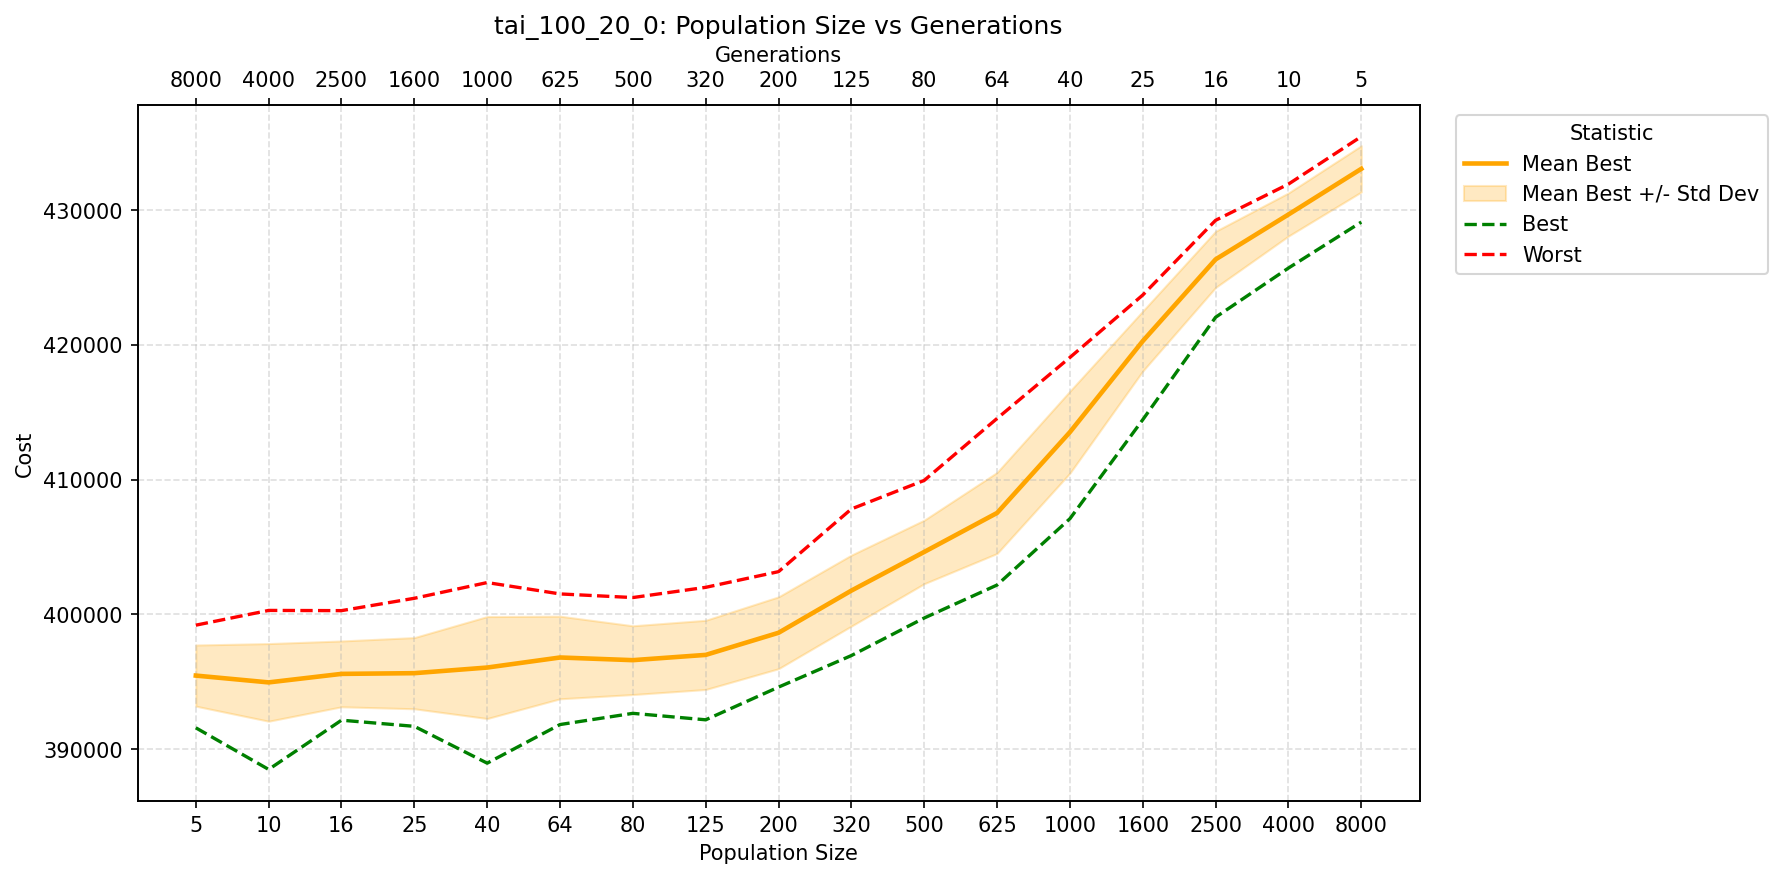
\includegraphics[width=0.48\textwidth]{../Experiments/01_default_evolutionary_population_generations/fig_tai_100_20_0_pair.png}
\hfill
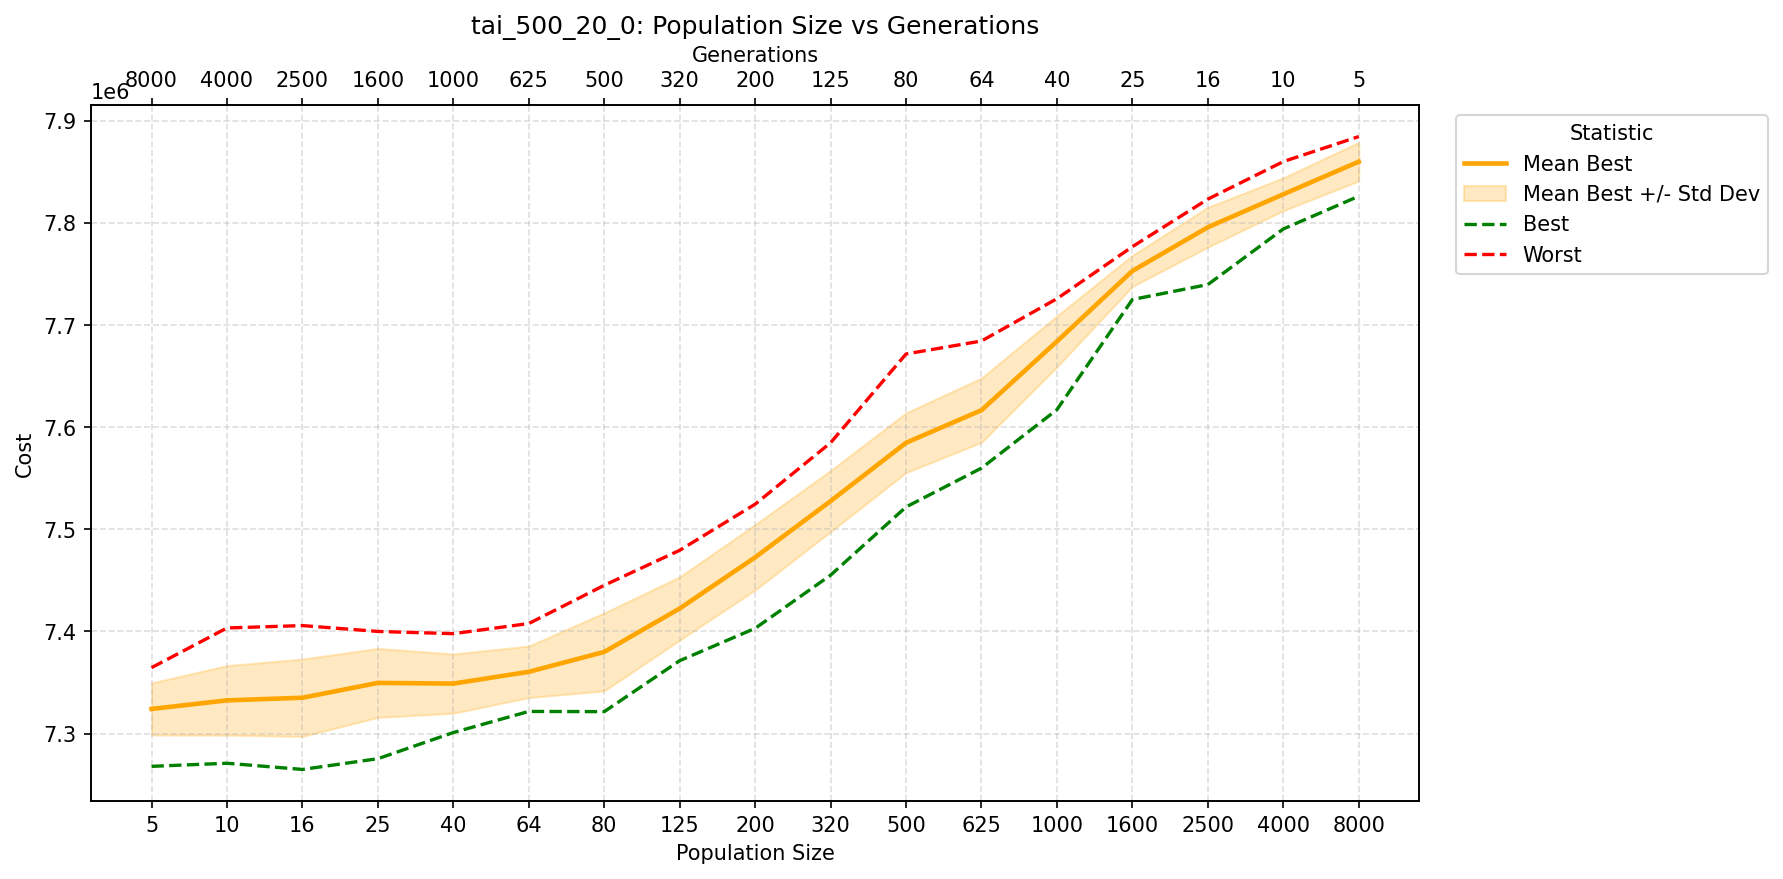
\includegraphics[width=0.48\textwidth]{../Experiments/01_default_evolutionary_population_generations/fig_tai_500_20_0_pair.png}
\caption{Pairwise population-size and generation-count analysis under tied \((P,G)\) settings. The lower axis shows population size, while the synchronized upper axis shows the bound generation count for each point.}
\label{fig:ea_pop_gen_pairwise_tai}
\end{figure}

\subsection*{Population Size and Generation Count Results Interpretation}



\section{Mutation Probability}

Mutation probability $p_{mut}$ is screened over a dense grid of 51 values from 0.0 to 1.0 (step 0.02) using the Swap mutation operator.
\begin{figure}[H]
\centering
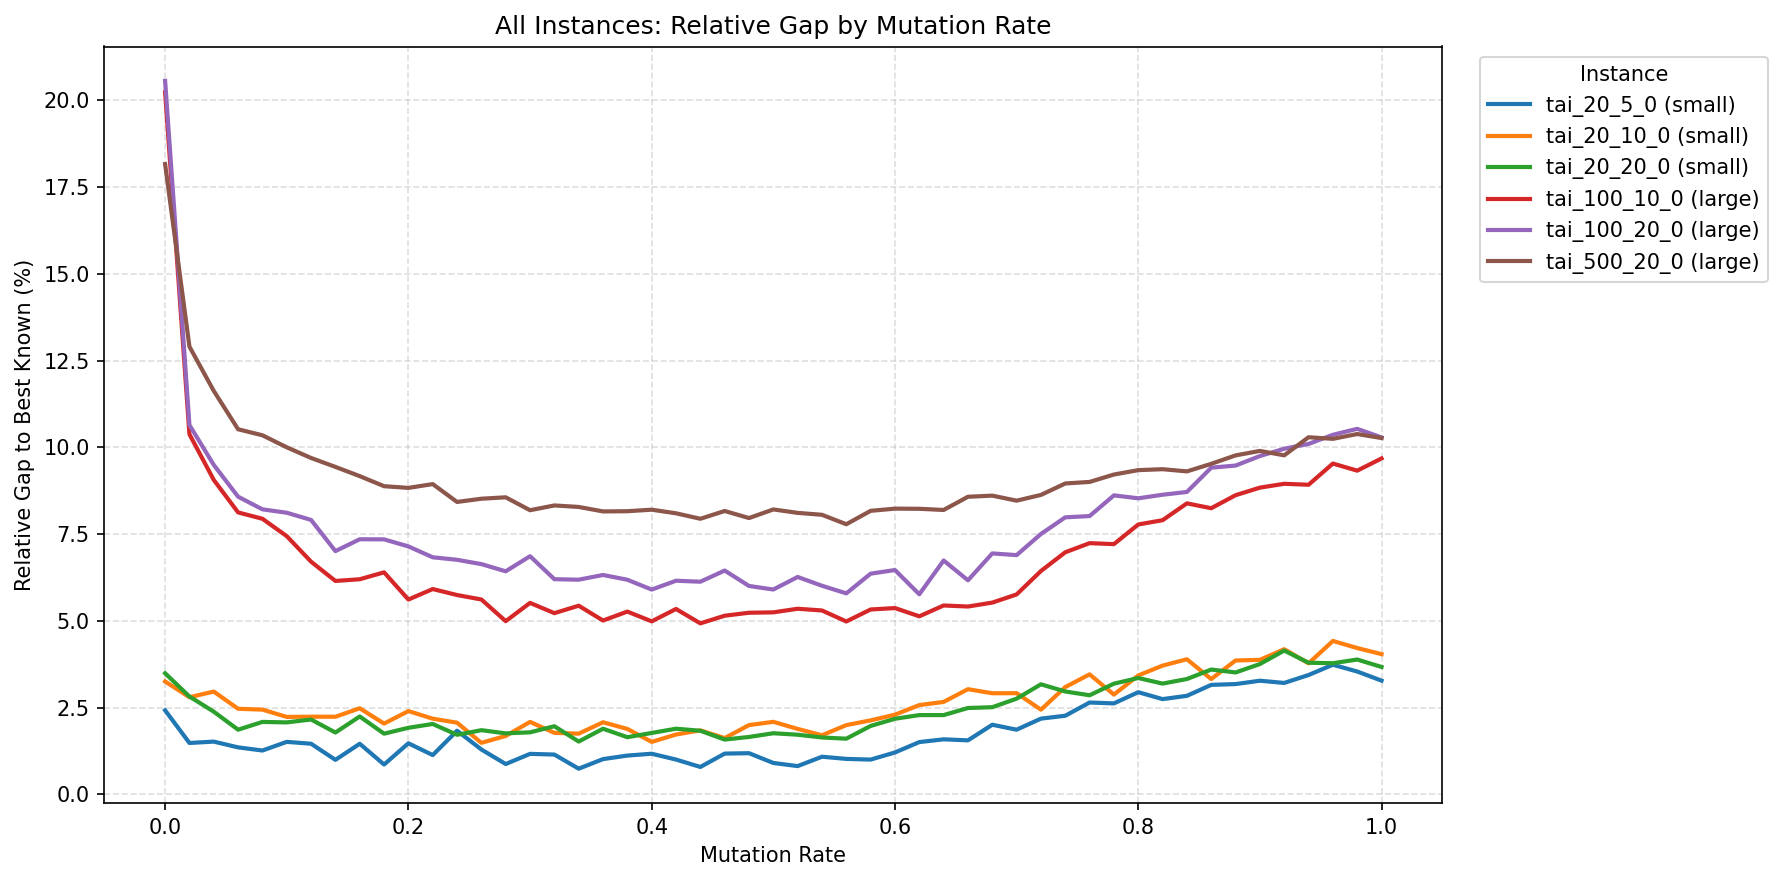
\includegraphics[width=0.96\textwidth]{../Experiments/04_evolutionary_mutation_grid/fig_mutation_all.png}
\caption{Mean relative gap to best-known values vs. mutation rate across all instances and both test sets.}
\label{fig:mutation_all}
\end{figure}

\begin{figure}[H]
\centering
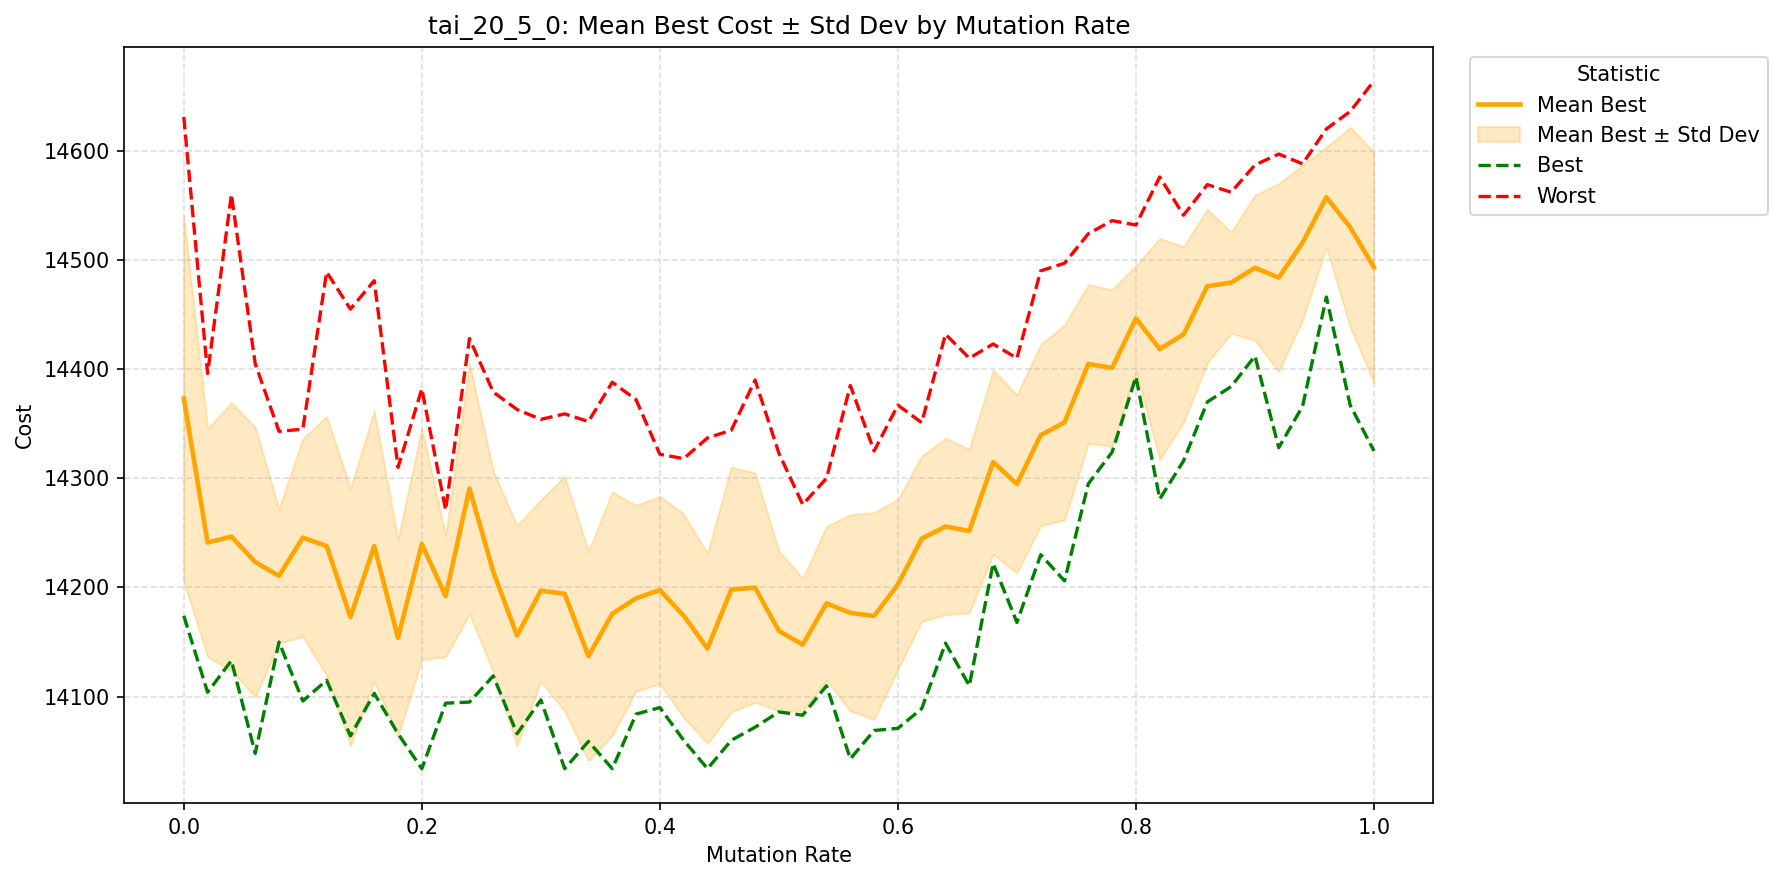
\includegraphics[width=0.48\textwidth]{../Experiments/04_evolutionary_mutation_grid/fig_mutation_tai_20_5_0.png}
\hfill
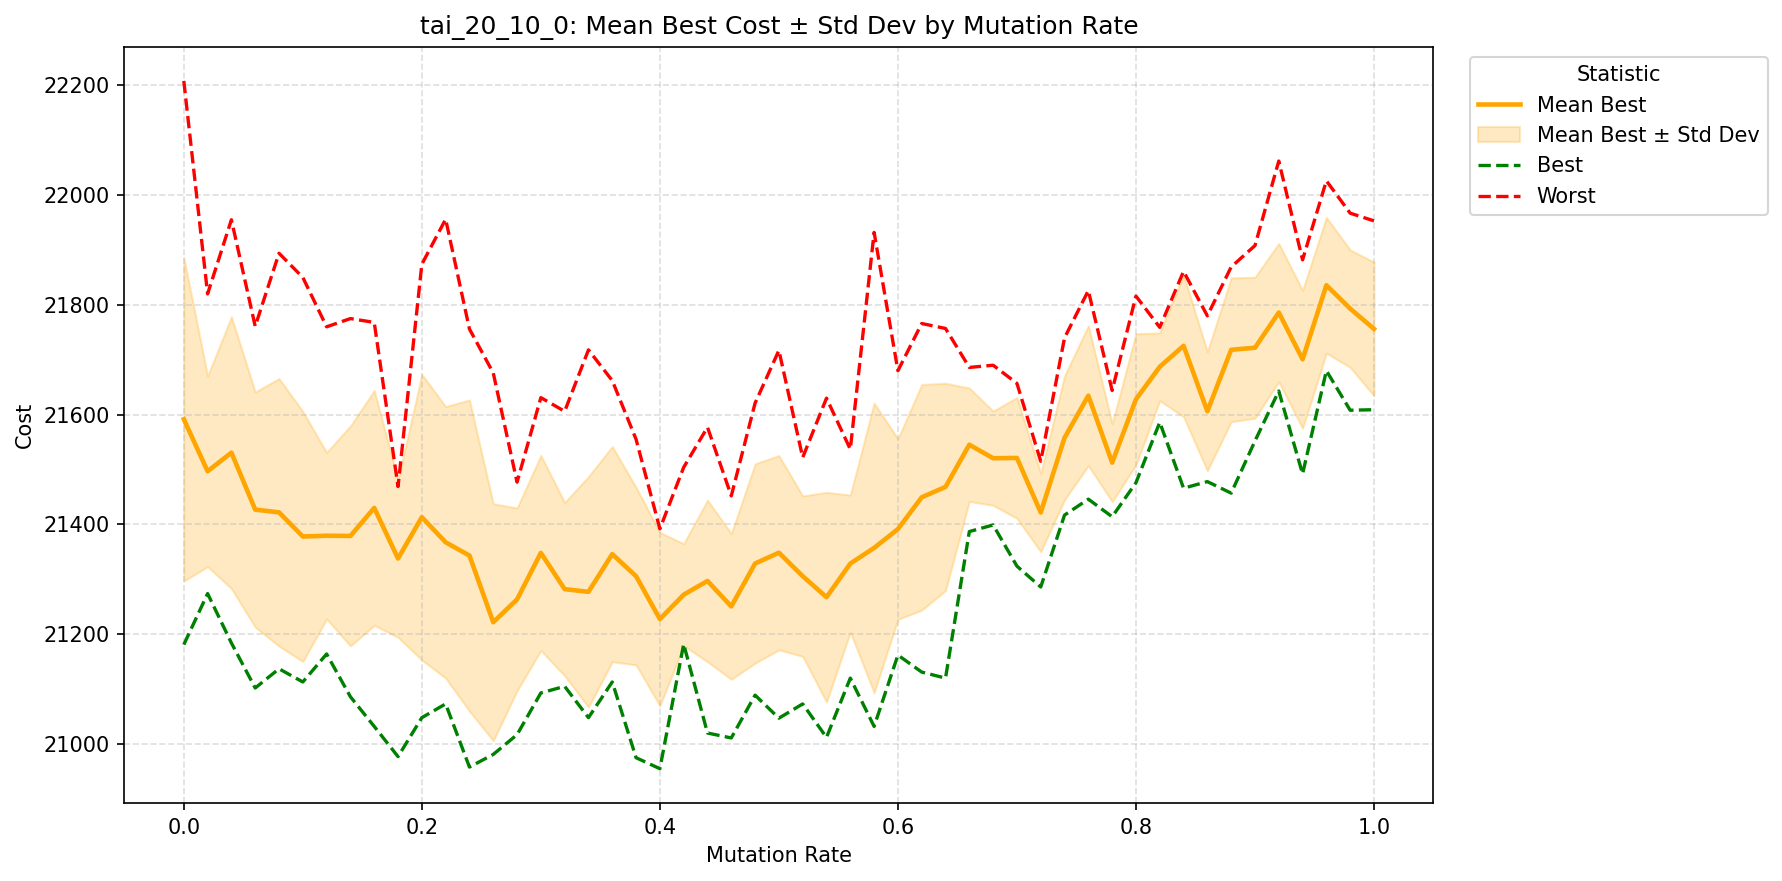
\includegraphics[width=0.48\textwidth]{../Experiments/04_evolutionary_mutation_grid/fig_mutation_tai_20_10_0.png}

\vspace{0.5em}

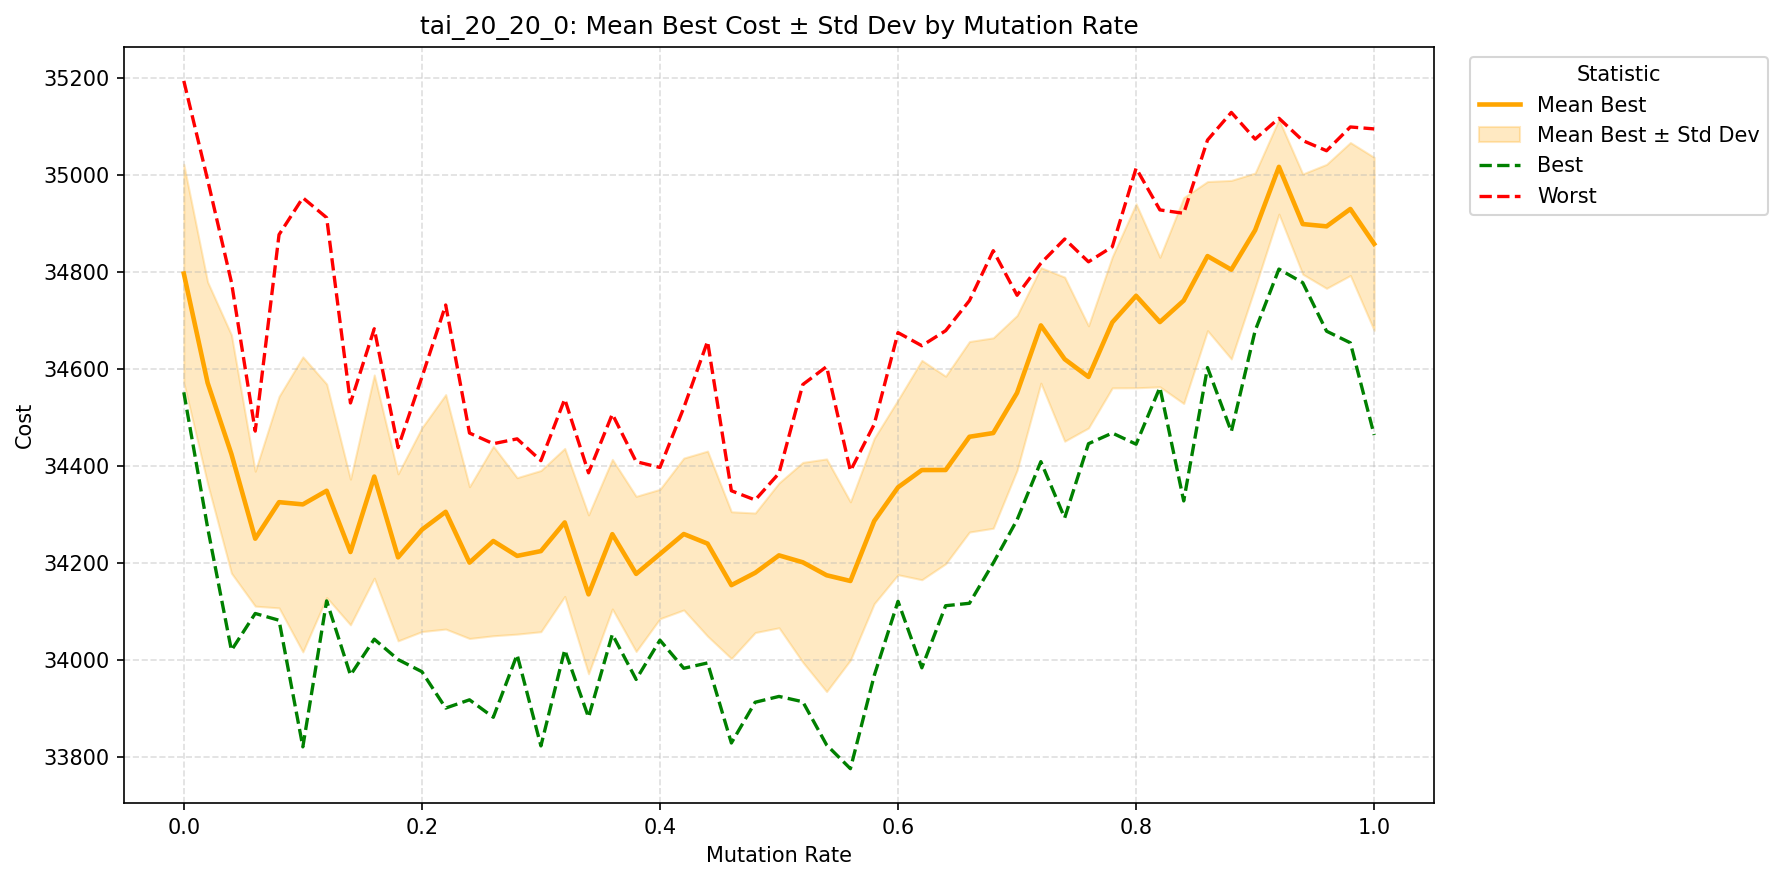
\includegraphics[width=0.48\textwidth]{../Experiments/04_evolutionary_mutation_grid/fig_mutation_tai_20_20_0.png}
\caption{Mutation rate sensitivity for small instances (\texttt{tai\_20\_*}).}
\label{fig:mutation_small}
\end{figure}

\begin{figure}[H]
\centering
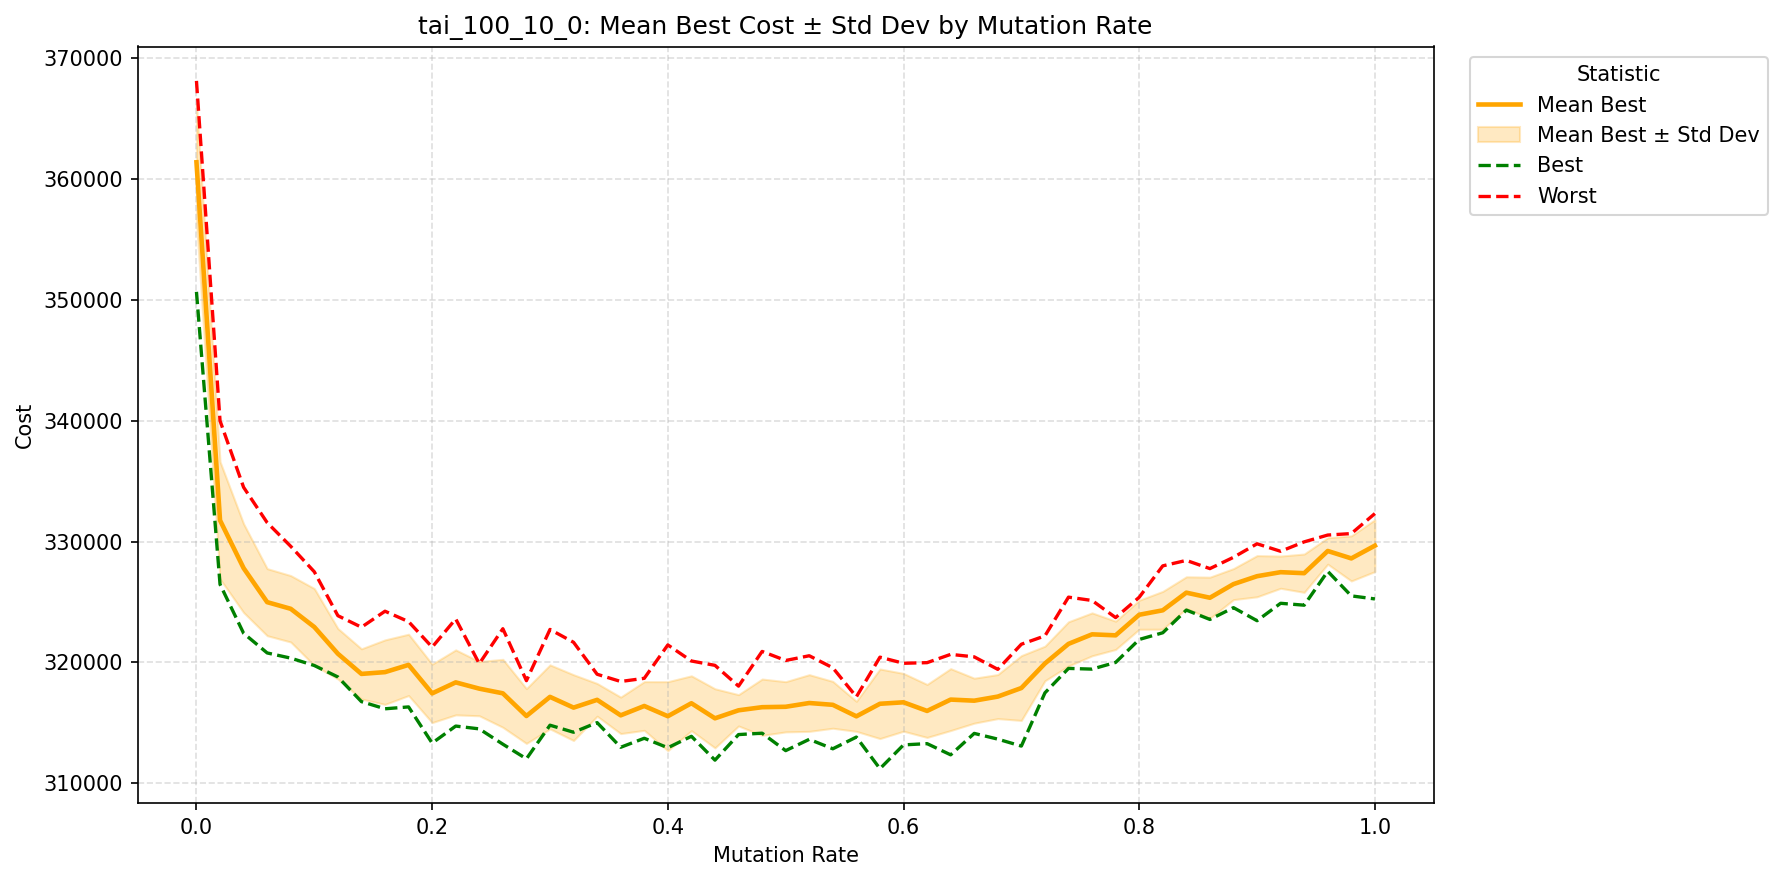
\includegraphics[width=0.48\textwidth]{../Experiments/04_evolutionary_mutation_grid/fig_mutation_tai_100_10_0.png}
\hfill
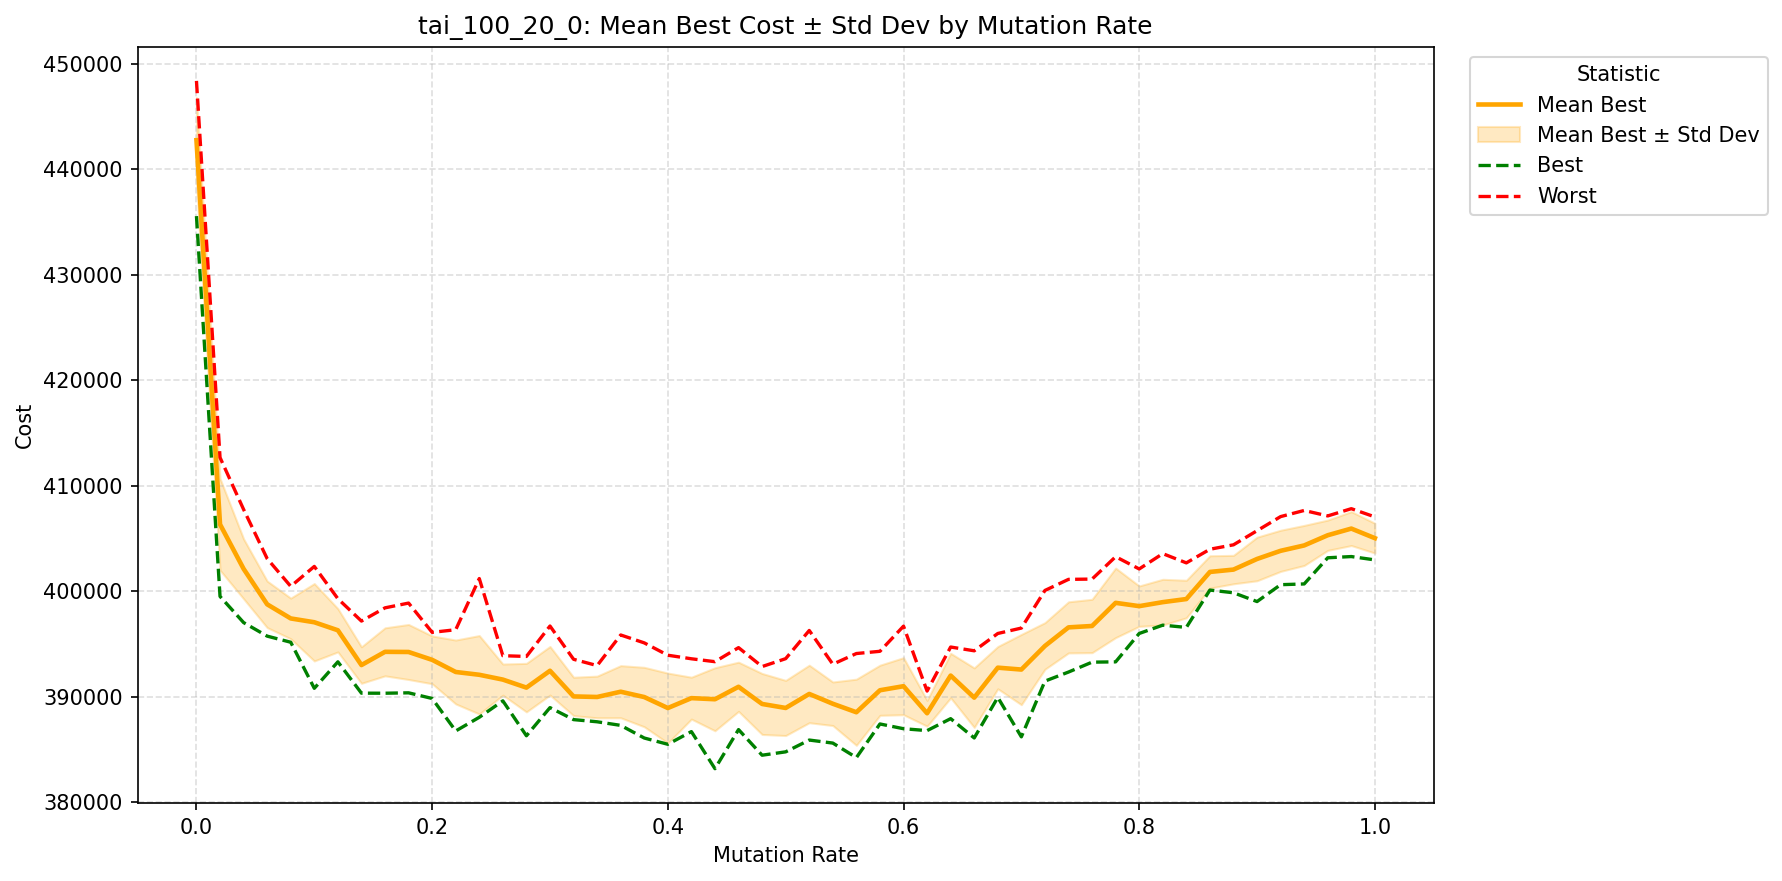
\includegraphics[width=0.48\textwidth]{../Experiments/04_evolutionary_mutation_grid/fig_mutation_tai_100_20_0.png}

\vspace{0.5em}

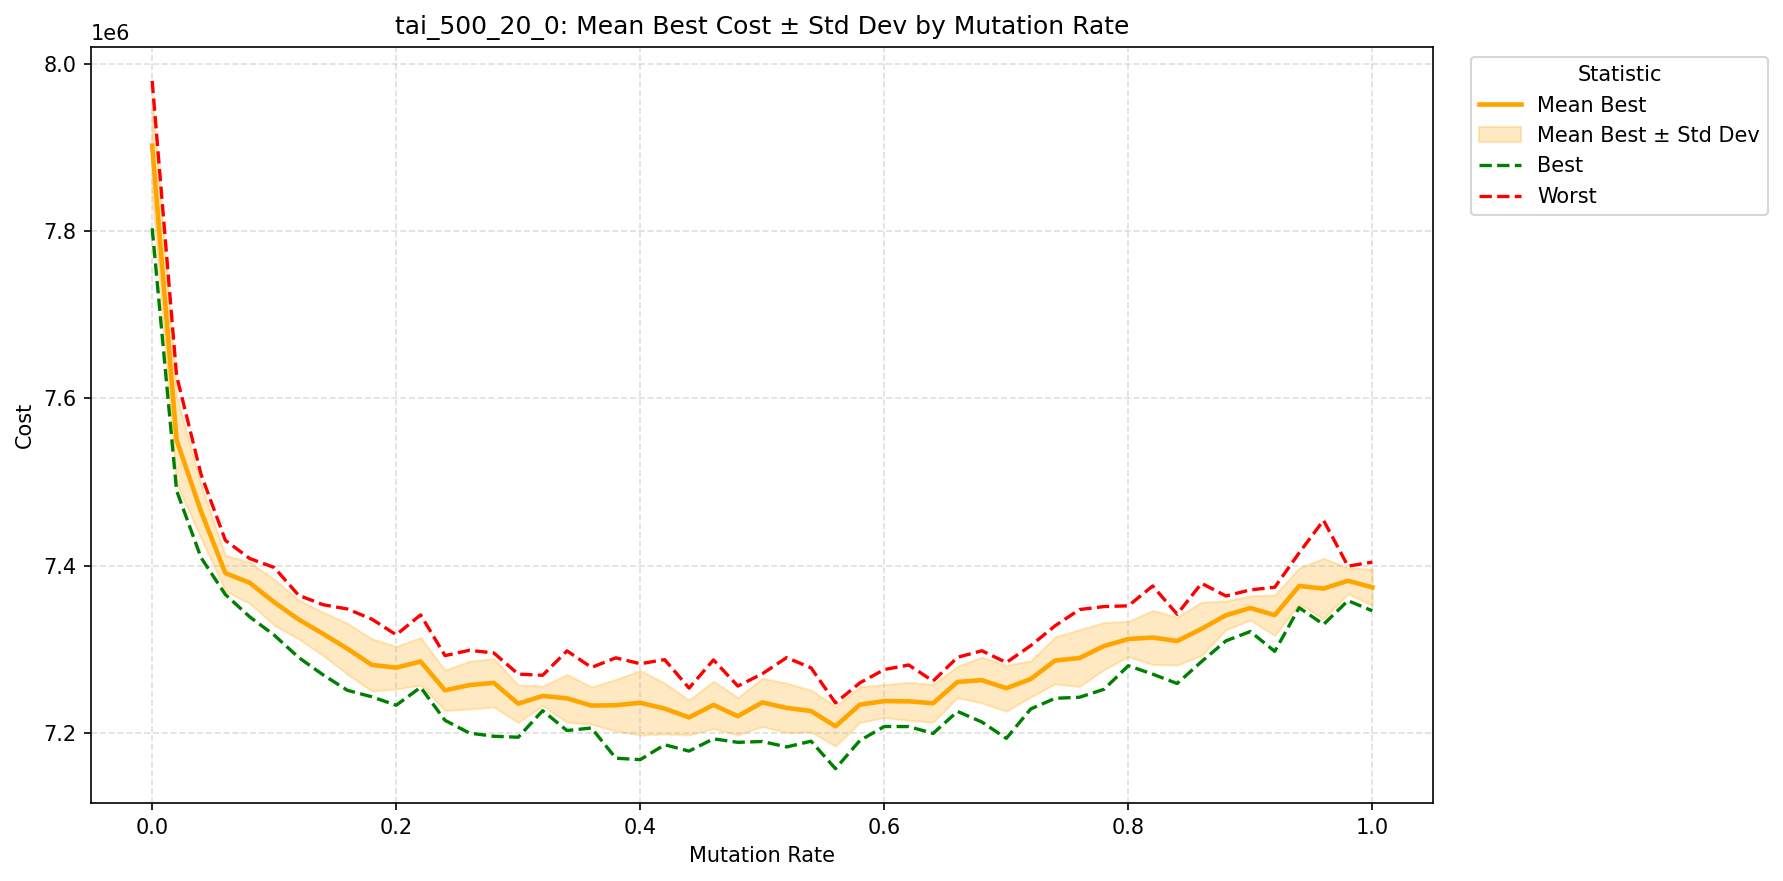
\includegraphics[width=0.48\textwidth]{../Experiments/04_evolutionary_mutation_grid/fig_mutation_tai_500_20_0.png}
\caption{Mutation rate sensitivity for large instances (\texttt{tai\_100\_*}, \texttt{tai\_500\_20\_0}).}
\label{fig:mutation_large}
\end{figure}


\section{Crossover Probability}
\begin{figure}[H]
\centering
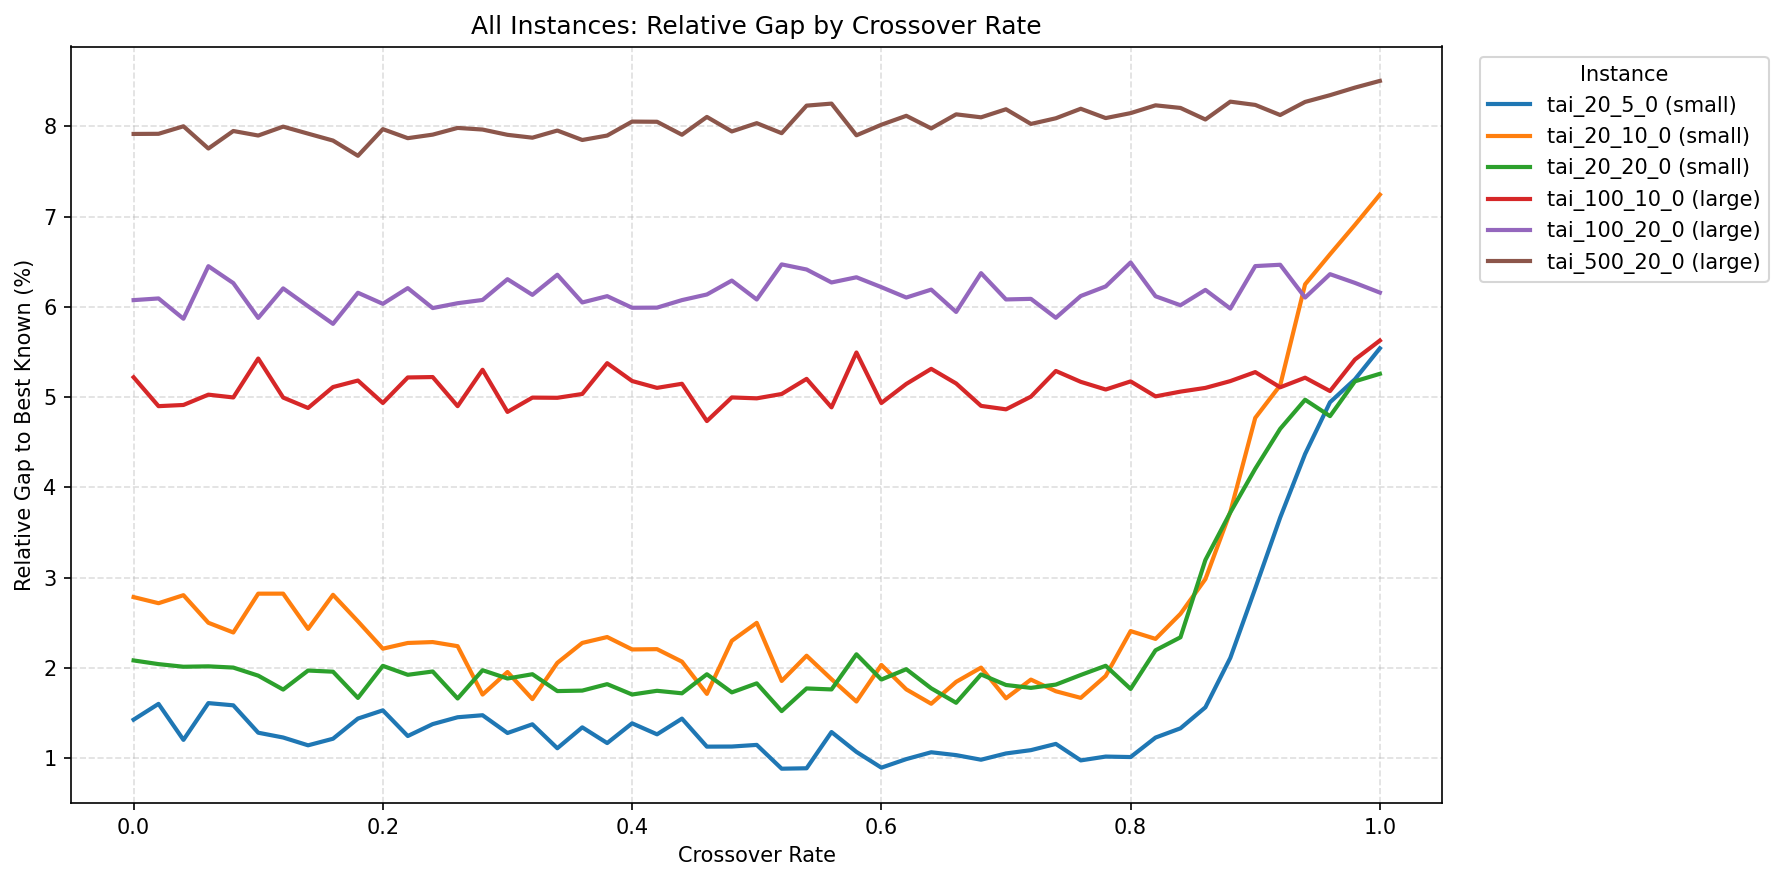
\includegraphics[width=0.96\textwidth]{../Experiments/05_evolutionary_crossover_grid/fig_crossover_all.png}
\caption{Mean relative gap to best-known values vs. crossover rate across all instances and both test sets.}
\label{fig:crossover_all}
\end{figure}

\begin{figure}[H]
\centering
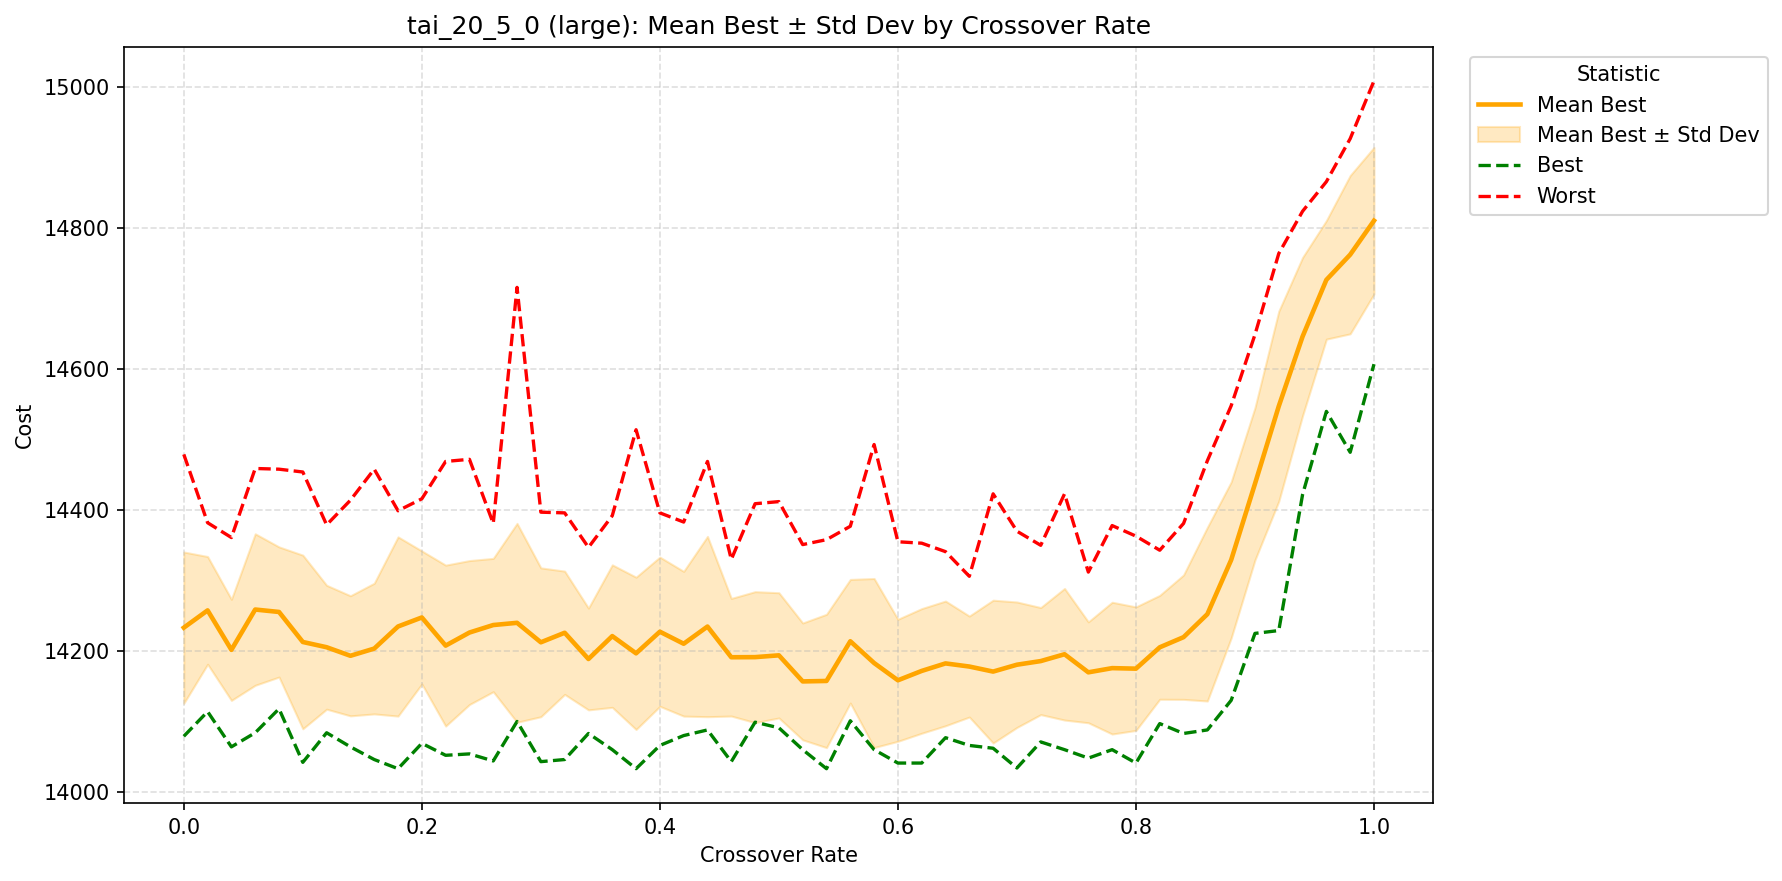
\includegraphics[width=0.48\textwidth]{../Experiments/05_evolutionary_crossover_grid/fig_crossover_tai_20_5_0.png}
\hfill
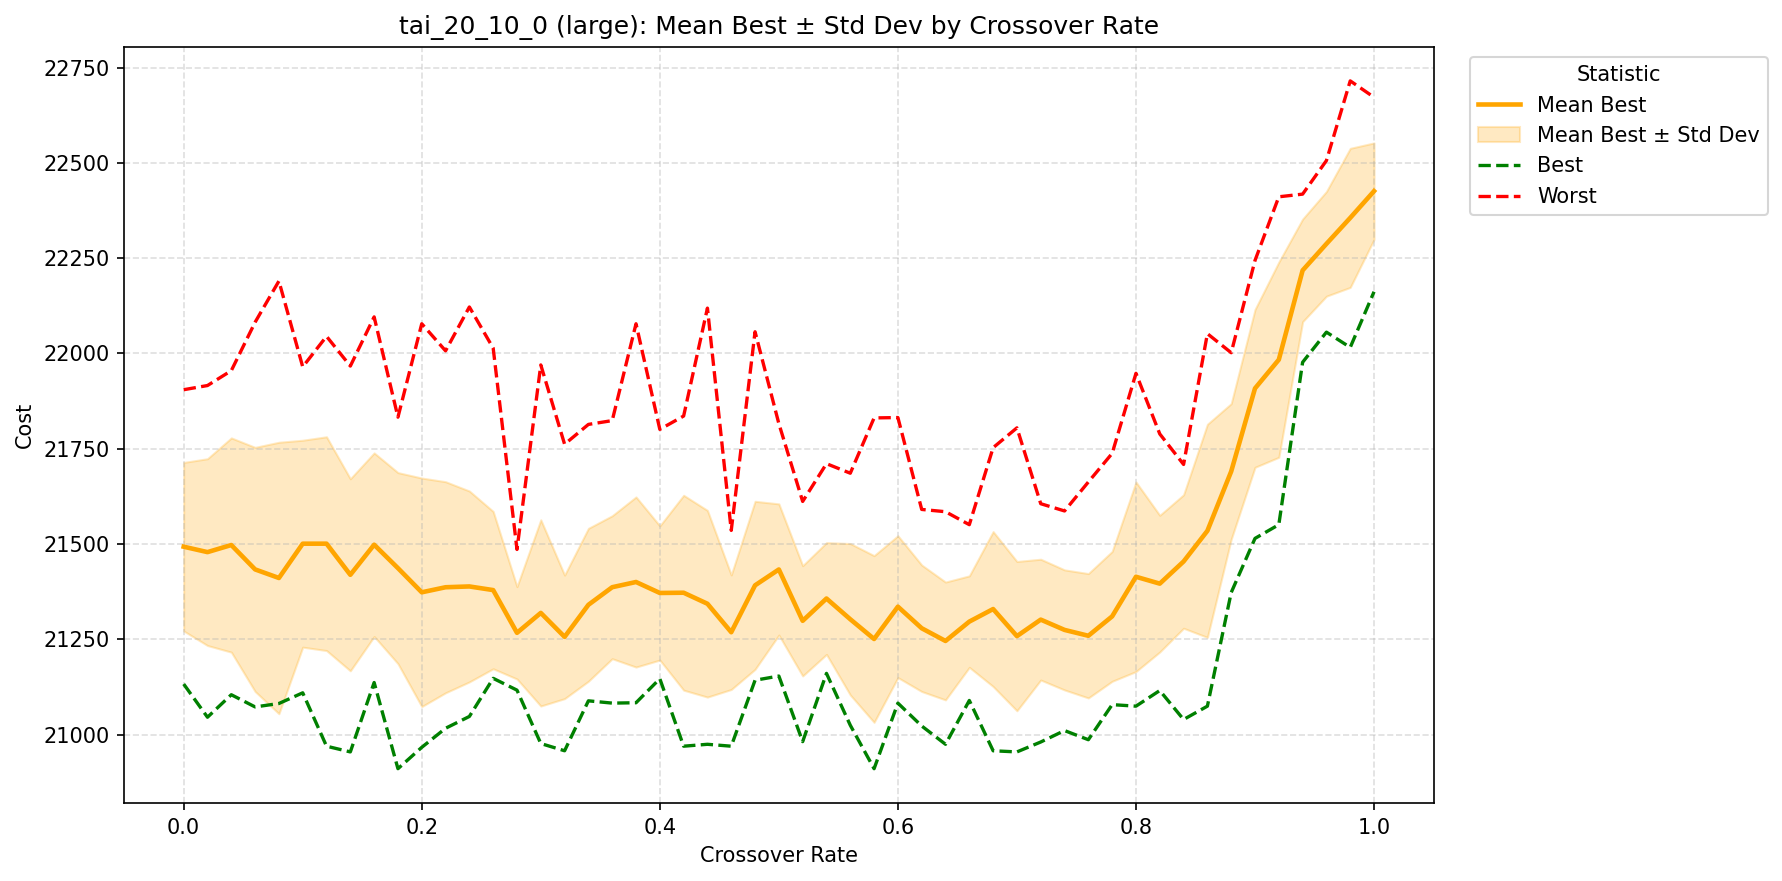
\includegraphics[width=0.48\textwidth]{../Experiments/05_evolutionary_crossover_grid/fig_crossover_tai_20_10_0.png}

\vspace{0.5em}

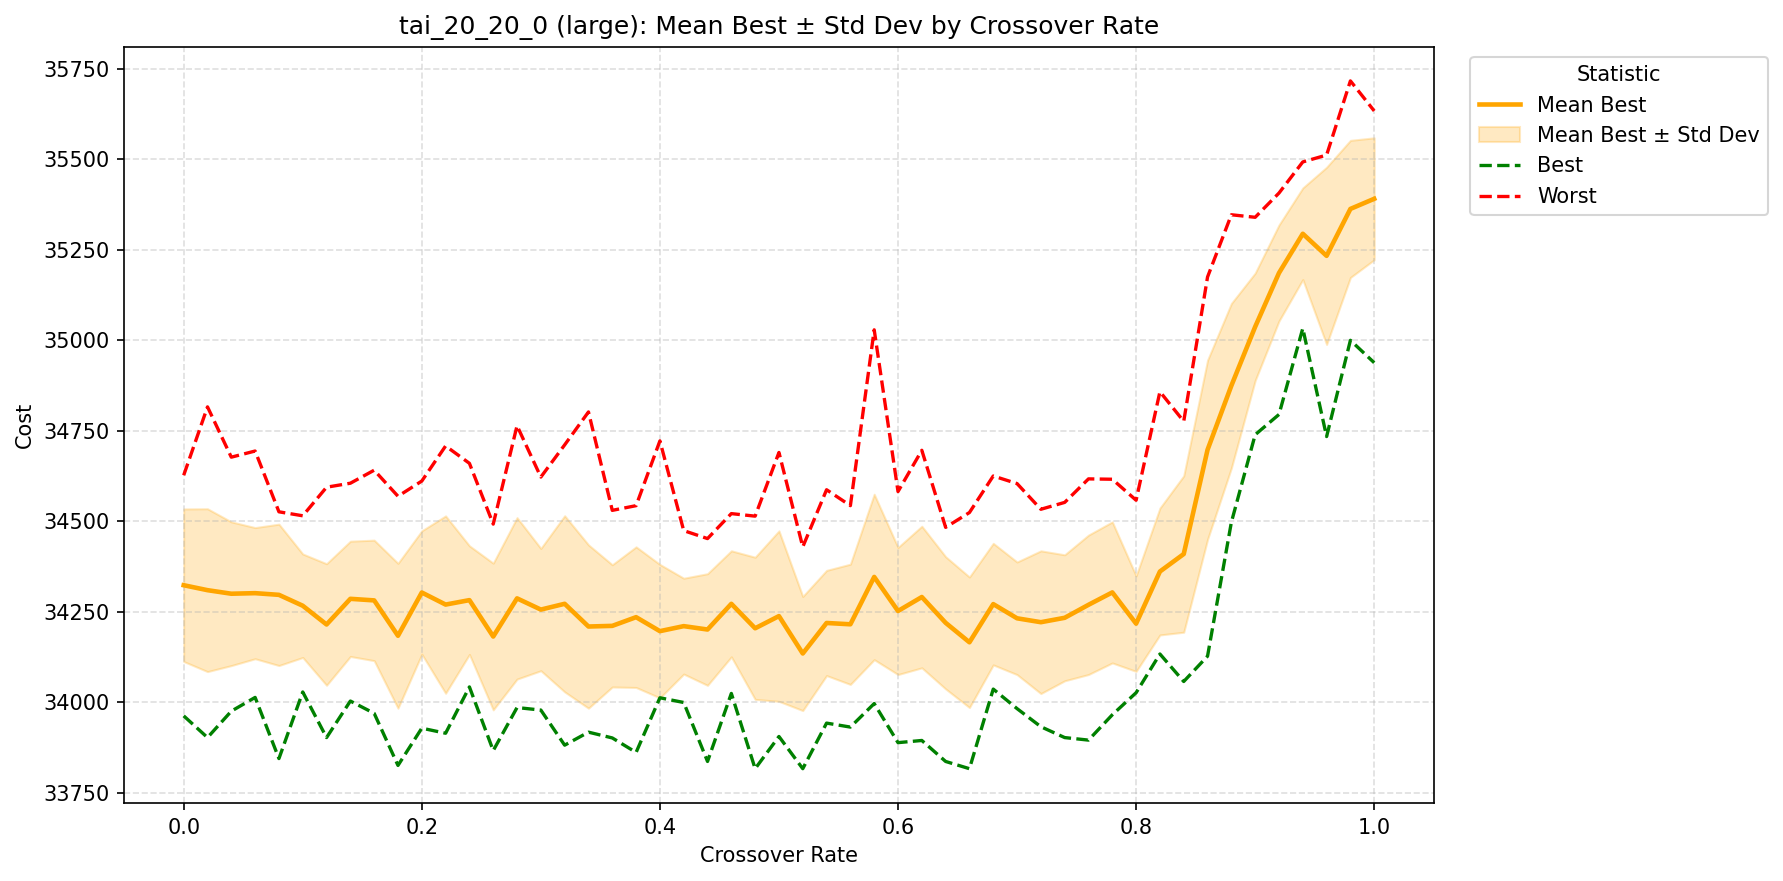
\includegraphics[width=0.48\textwidth]{../Experiments/05_evolutionary_crossover_grid/fig_crossover_tai_20_20_0.png}
\caption{Crossover rate sensitivity for small instances (\texttt{tai\_20\_*}).}
\label{fig:crossover_small}
\end{figure}

\begin{figure}[H]
\centering
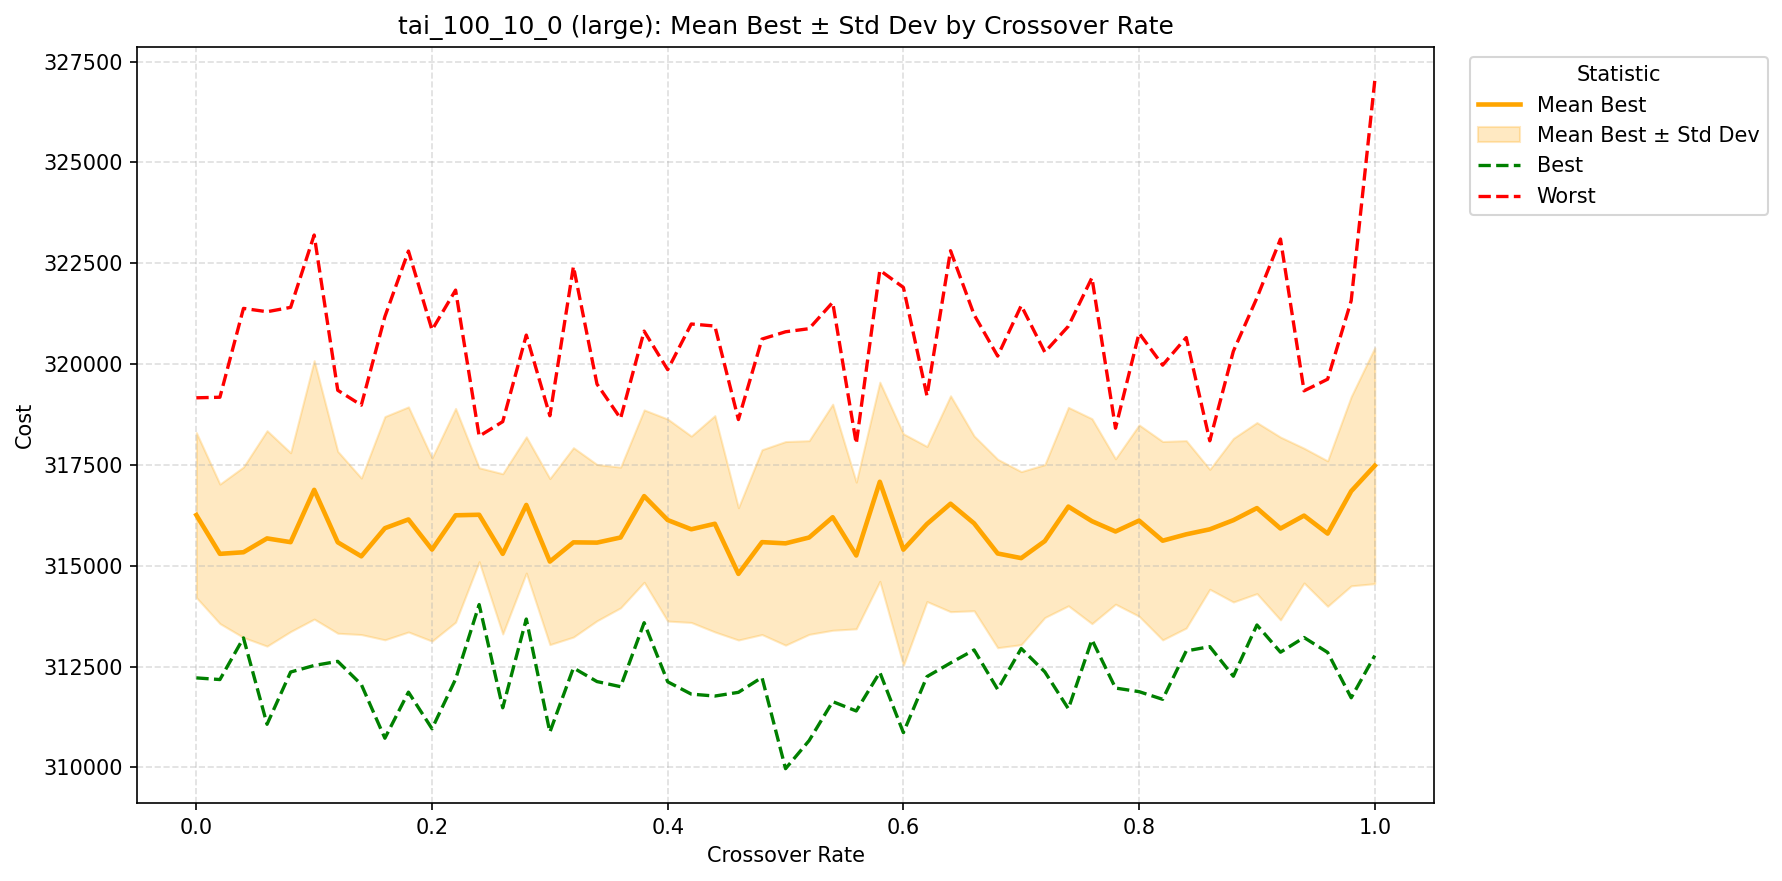
\includegraphics[width=0.48\textwidth]{../Experiments/05_evolutionary_crossover_grid/fig_crossover_tai_100_10_0.png}
\hfill
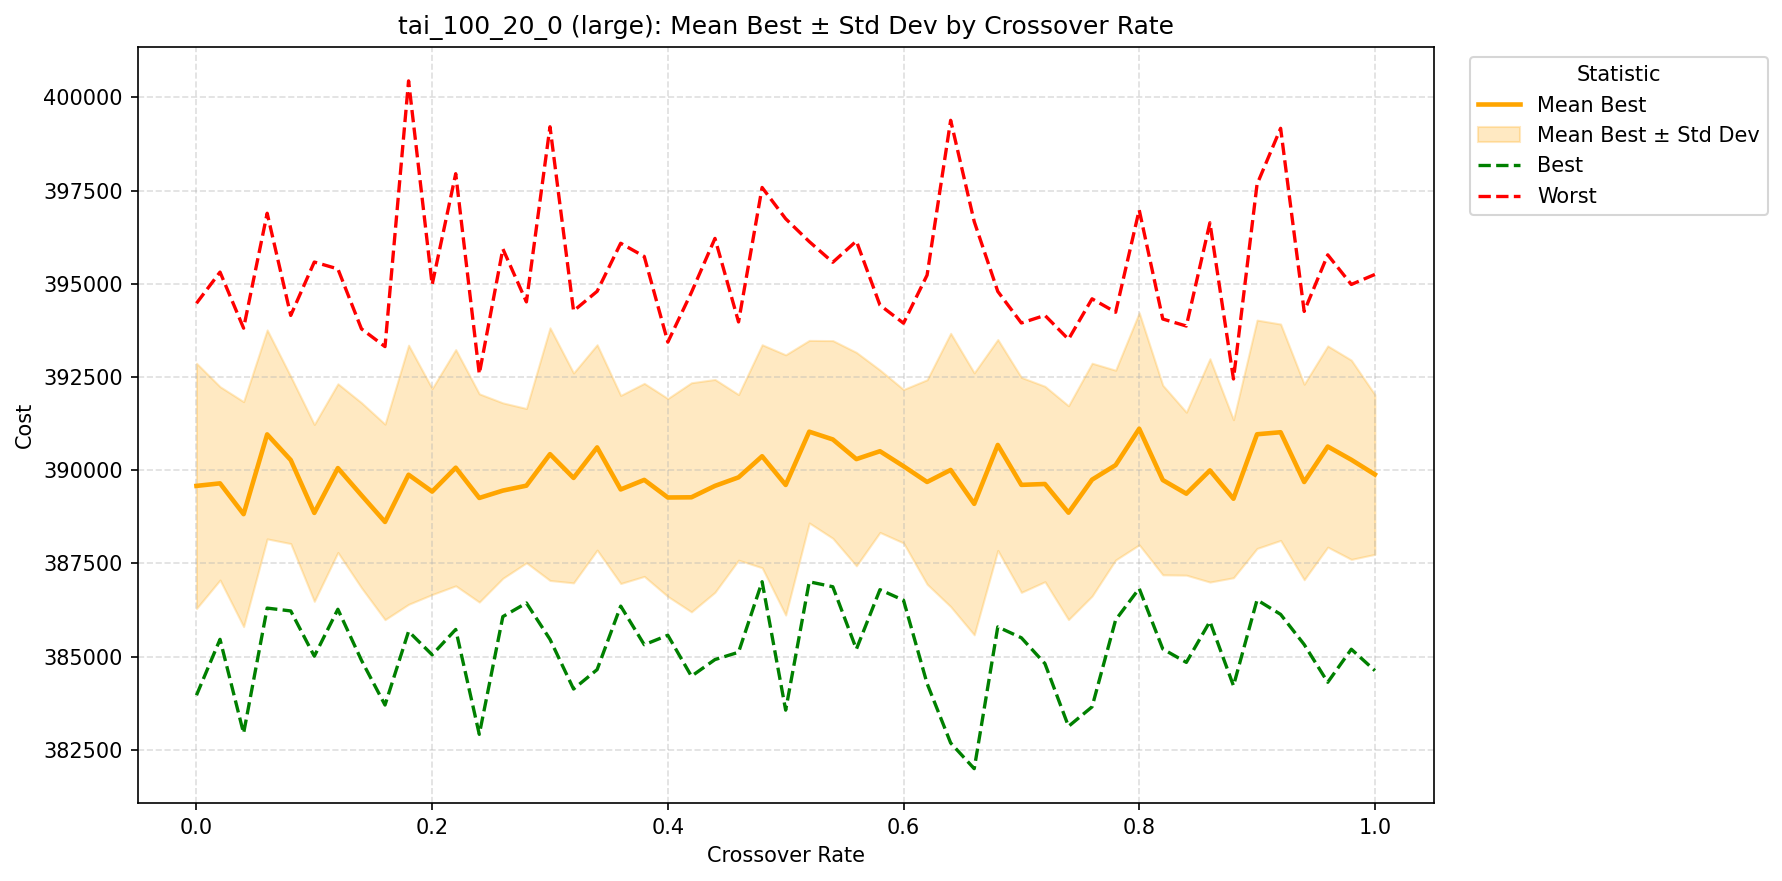
\includegraphics[width=0.48\textwidth]{../Experiments/05_evolutionary_crossover_grid/fig_crossover_tai_100_20_0.png}

\vspace{0.5em}

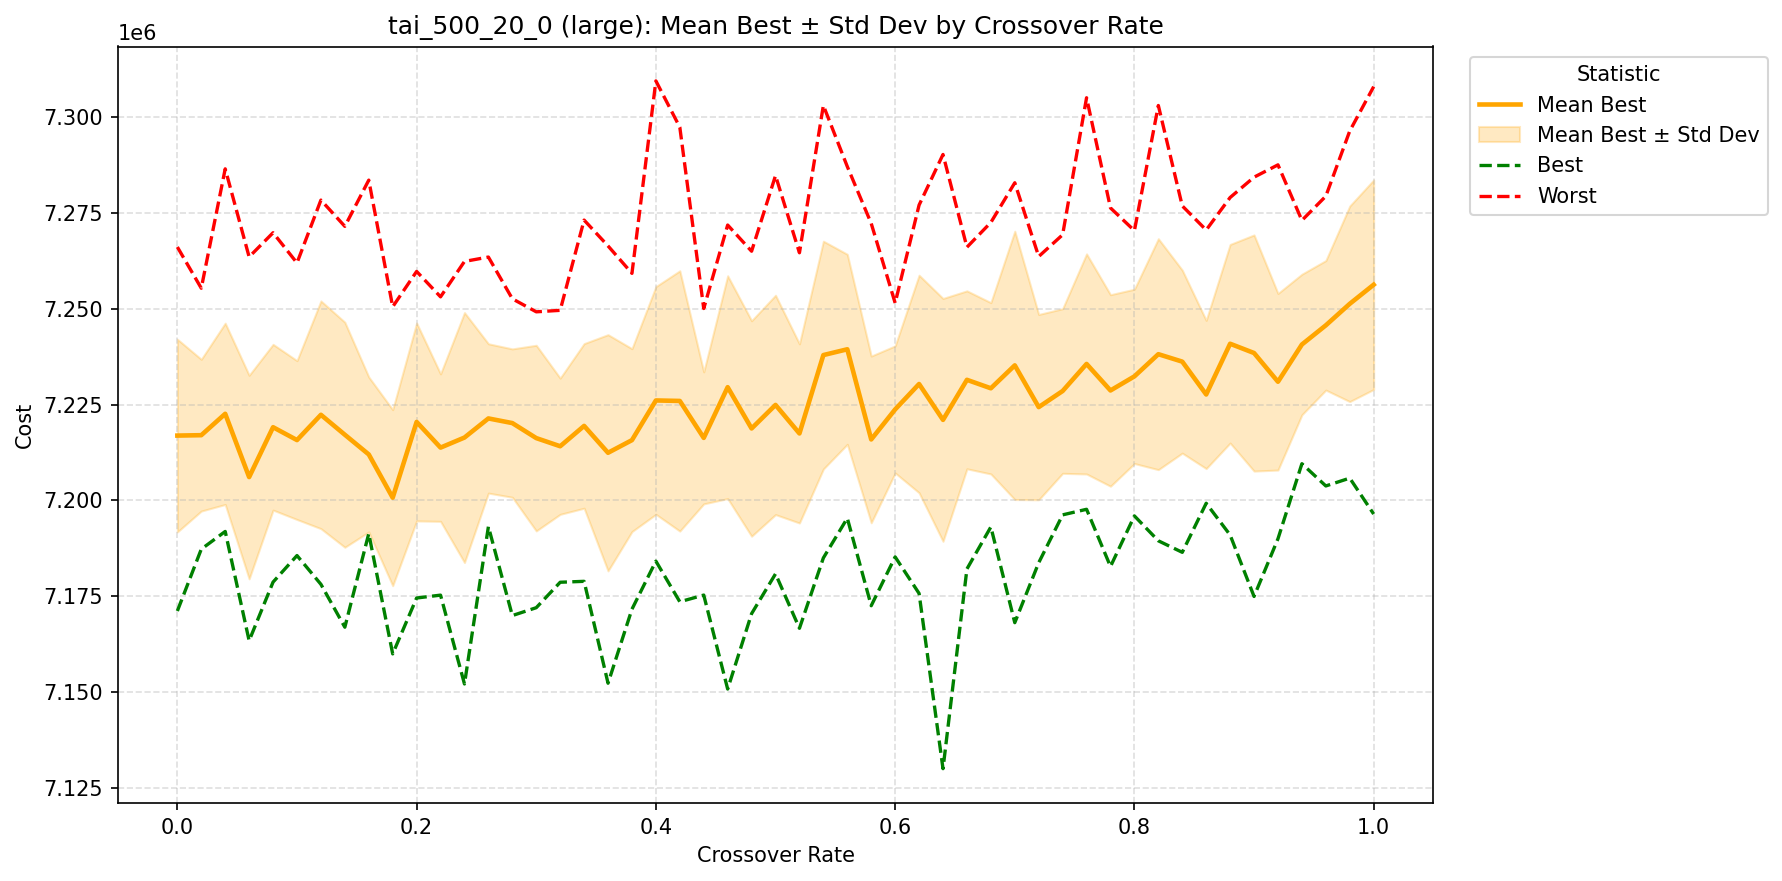
\includegraphics[width=0.48\textwidth]{../Experiments/05_evolutionary_crossover_grid/fig_crossover_tai_500_20_0.png}
\caption{Crossover rate sensitivity for large instances (\texttt{tai\_100\_*}, \texttt{tai\_500\_20\_0}).}
\label{fig:crossover_large}
\end{figure}

\section{Tournament Size}

\begin{figure}[H]
\centering
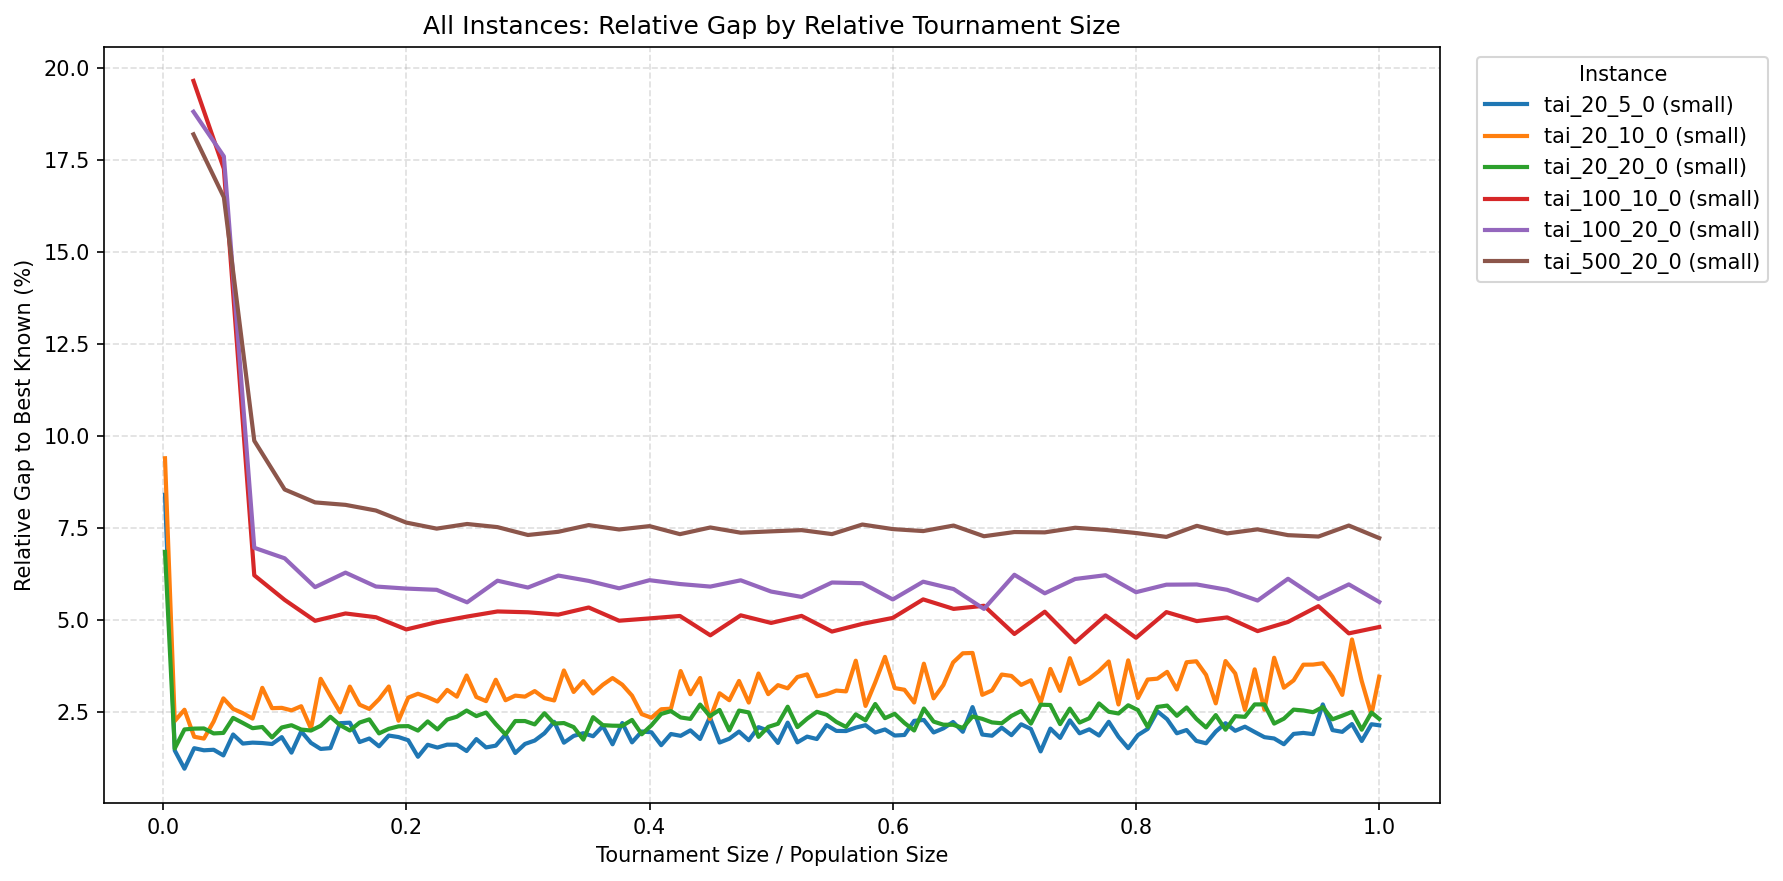
\includegraphics[width=0.96\textwidth]{../Experiments/06_evolutionary_tournament_grid/fig_tournament_all.png}
\caption{Mean relative gap to best-known values vs. tournament size across all instances and both test sets.}
\label{fig:tournament_all}
\end{figure}

\begin{figure}[H]
\centering
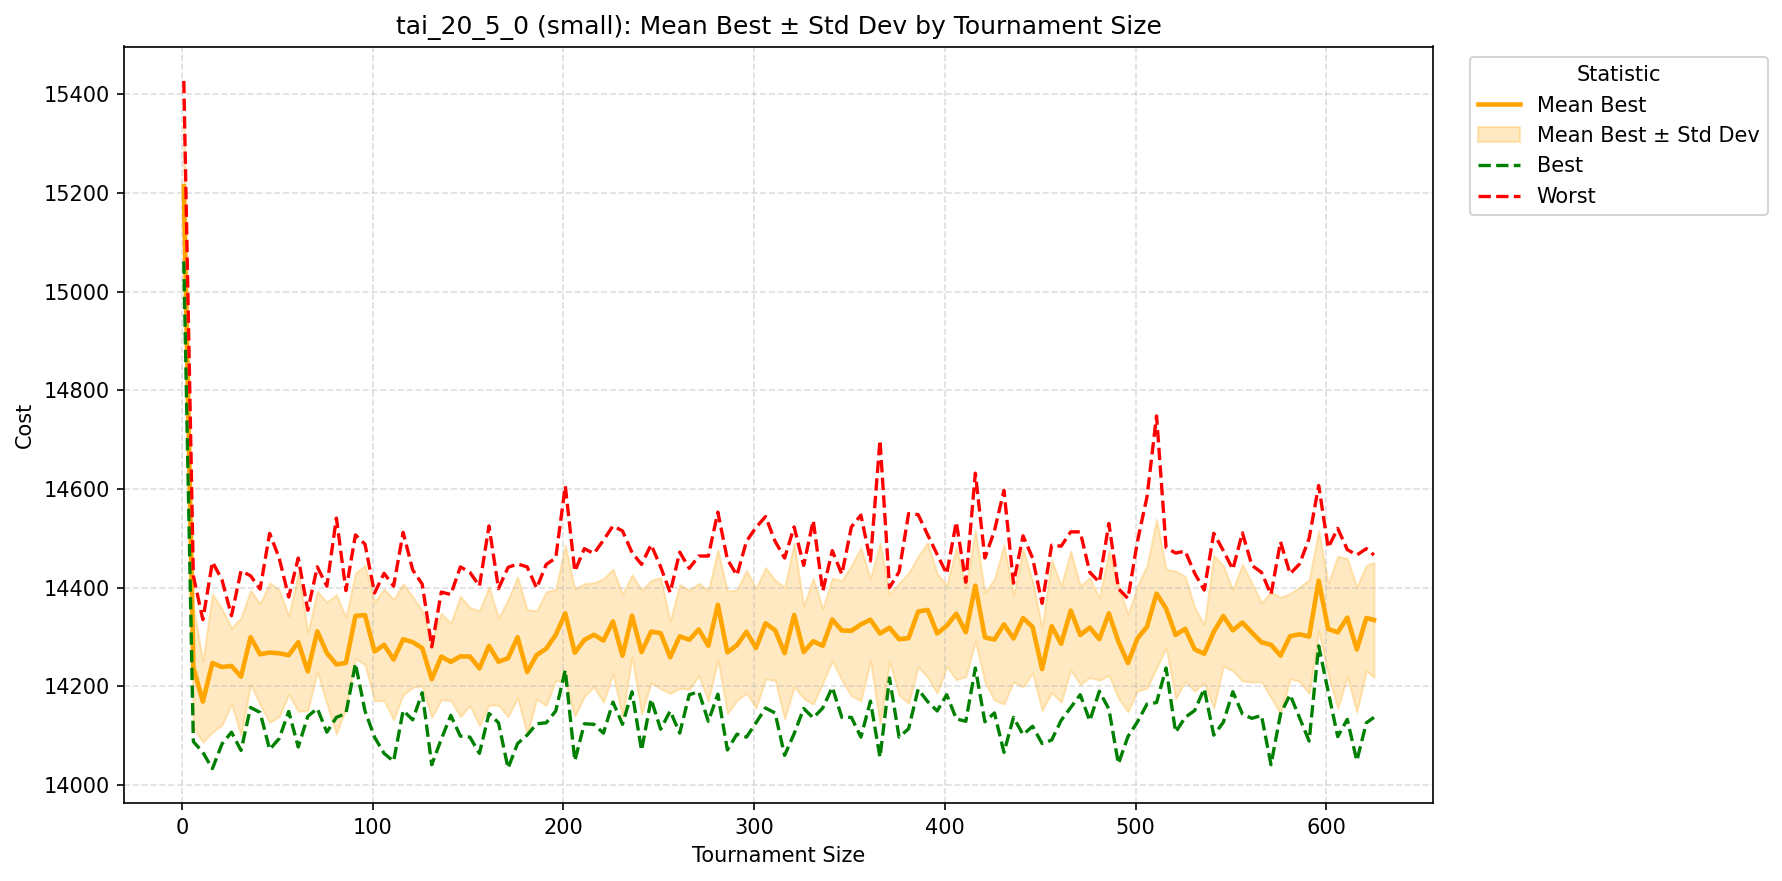
\includegraphics[width=0.48\textwidth]{../Experiments/06_evolutionary_tournament_grid/fig_tournament_tai_20_5_0.png}
\hfill
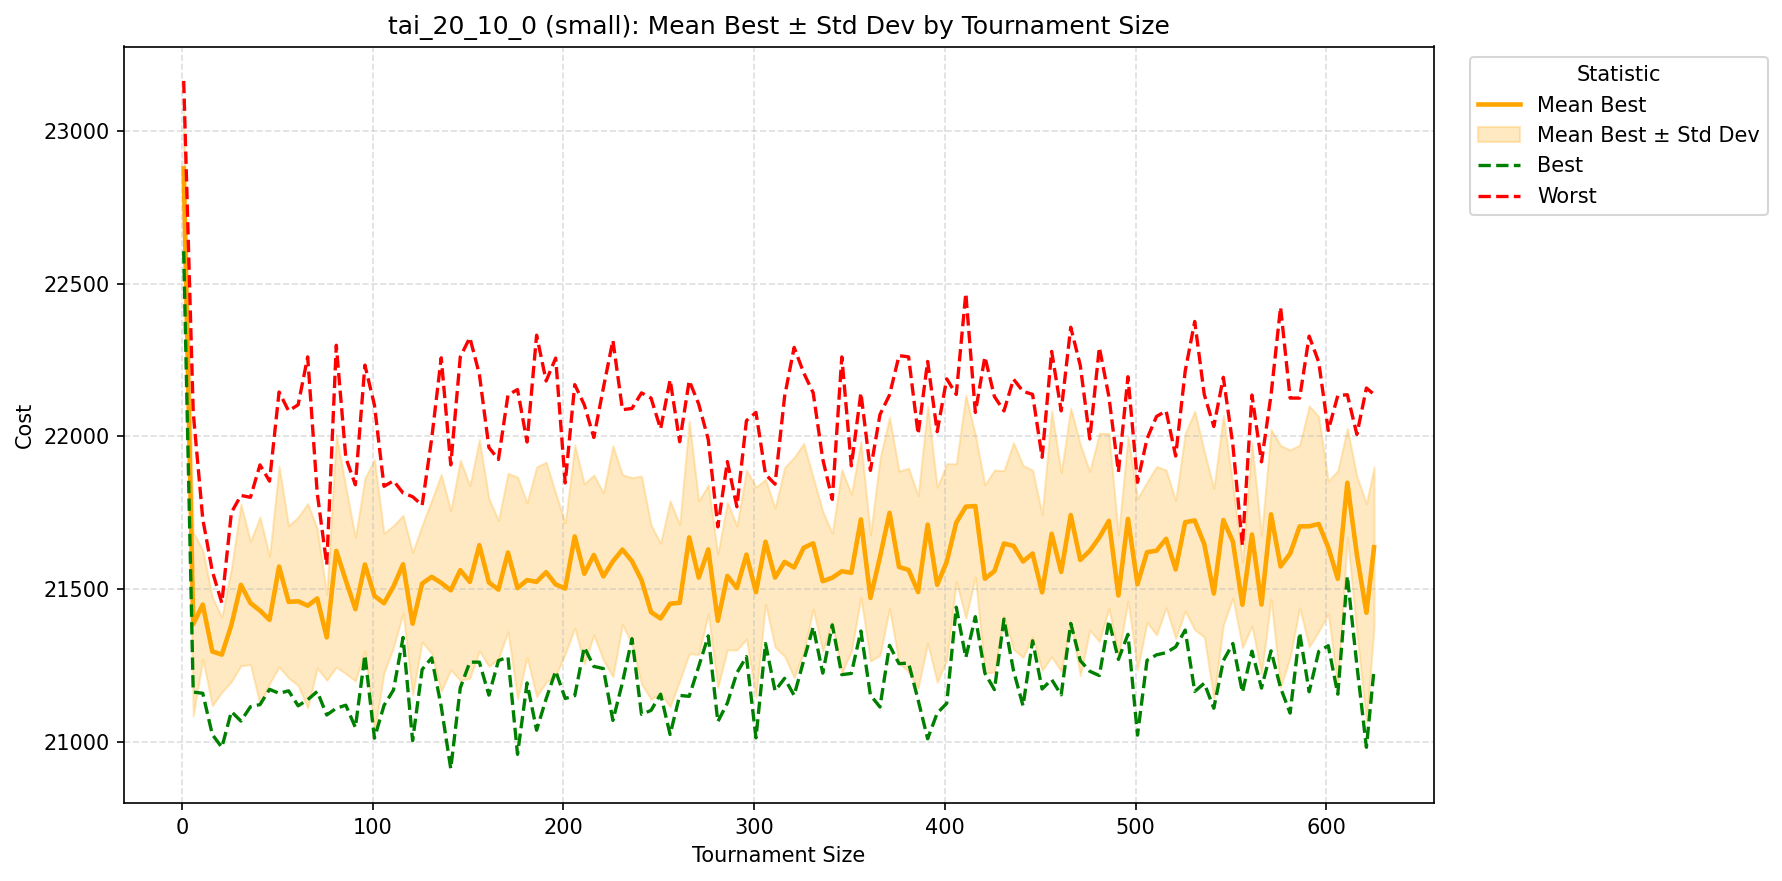
\includegraphics[width=0.48\textwidth]{../Experiments/06_evolutionary_tournament_grid/fig_tournament_tai_20_10_0.png}

\vspace{0.5em}

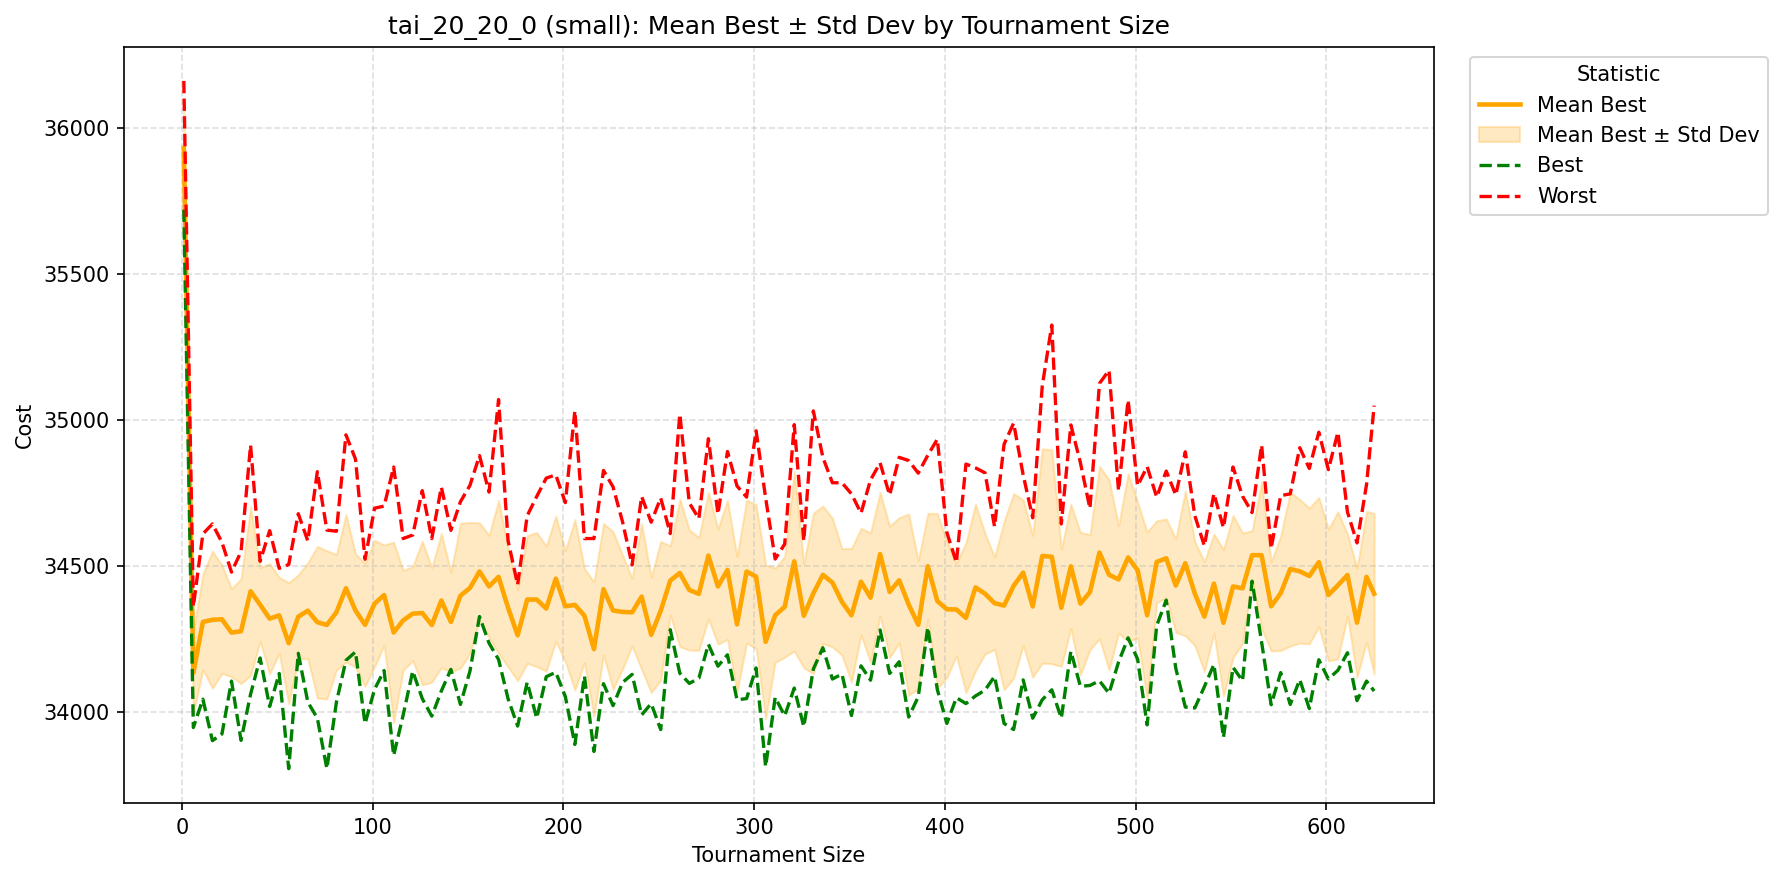
\includegraphics[width=0.48\textwidth]{../Experiments/06_evolutionary_tournament_grid/fig_tournament_tai_20_20_0.png}
\caption{Tournament size sensitivity for small instances (\texttt{tai\_20\_*}).}
\label{fig:tournament_small}
\end{figure}

\begin{figure}[H]
\centering
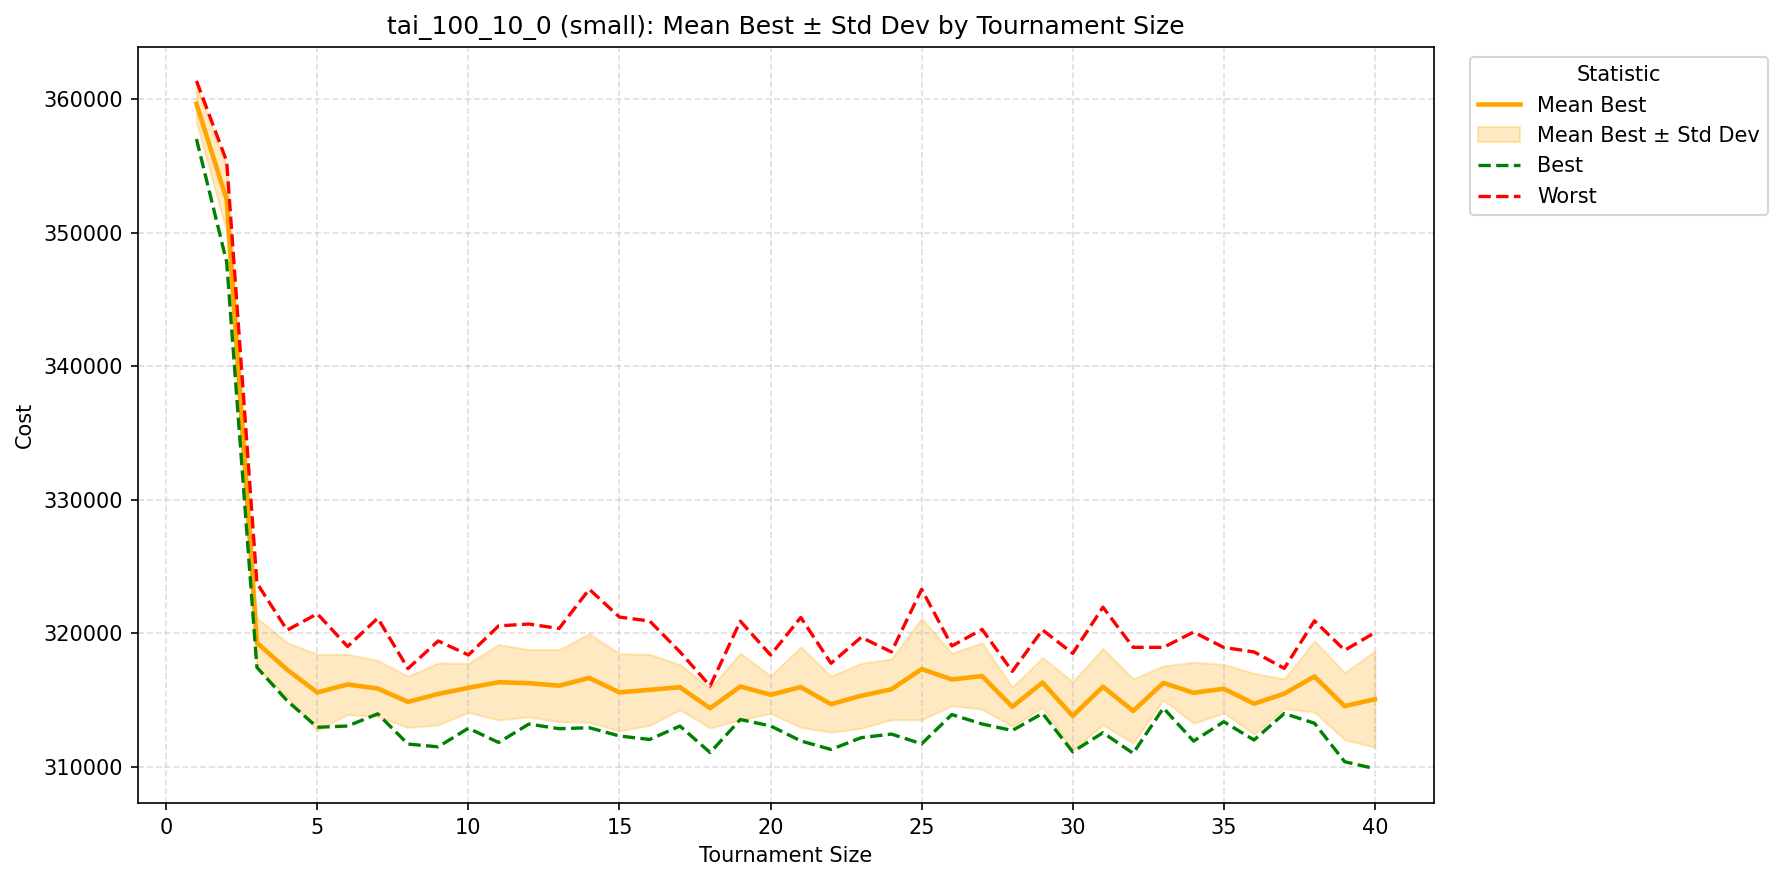
\includegraphics[width=0.48\textwidth]{../Experiments/06_evolutionary_tournament_grid/fig_tournament_tai_100_10_0.png}
\hfill
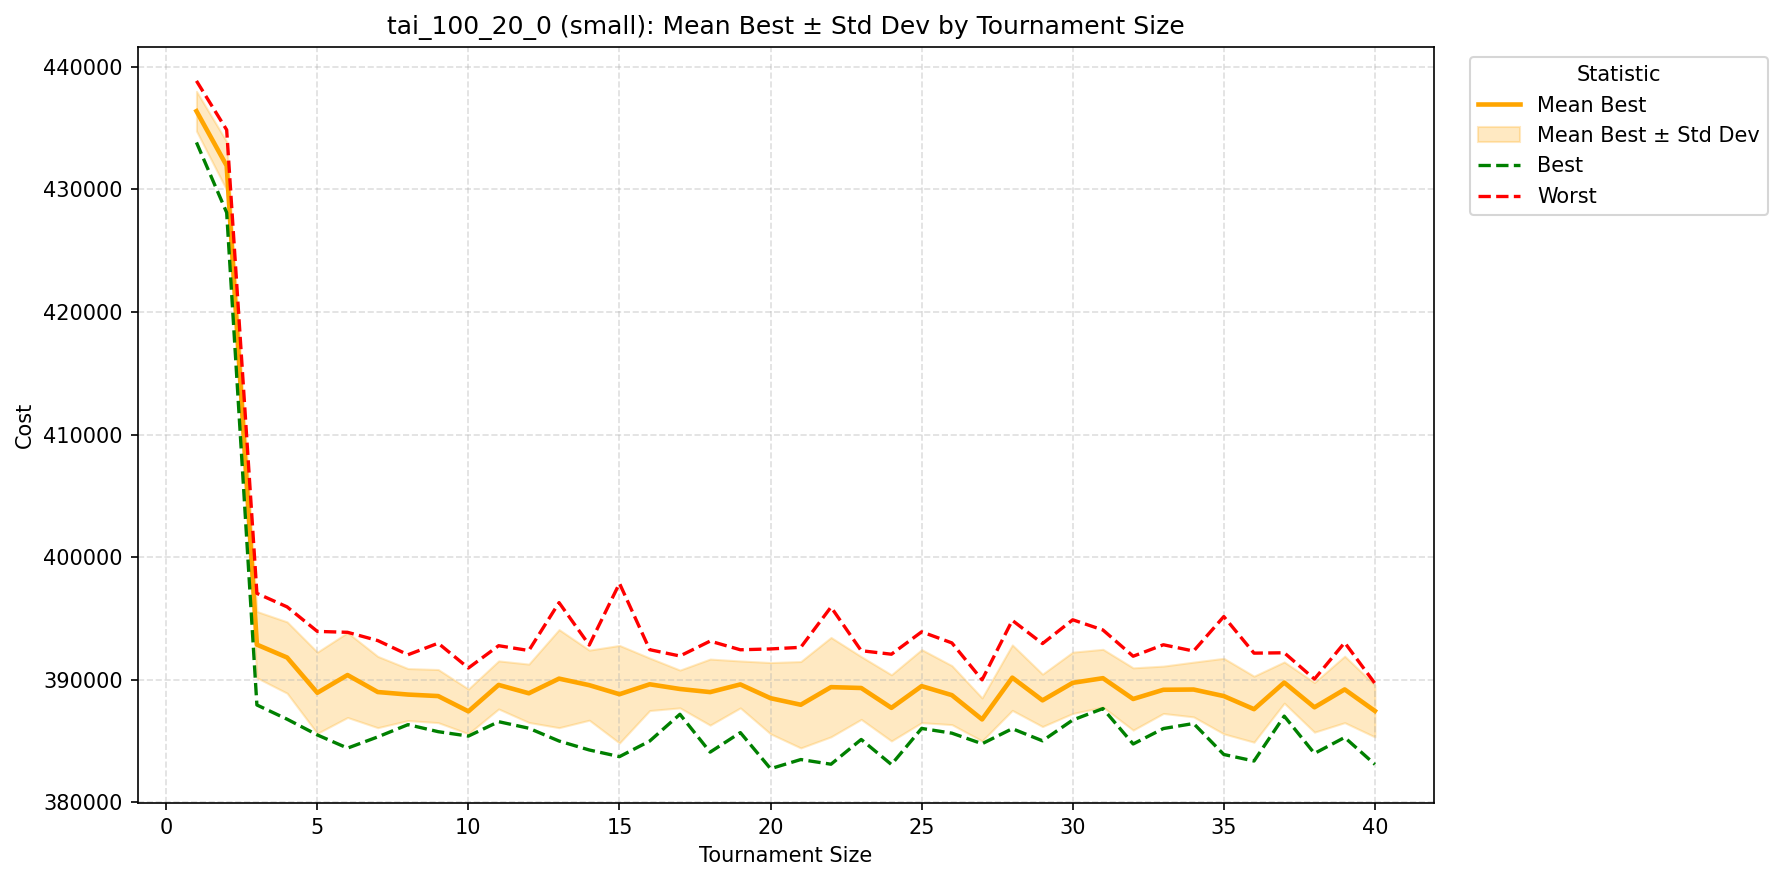
\includegraphics[width=0.48\textwidth]{../Experiments/06_evolutionary_tournament_grid/fig_tournament_tai_100_20_0.png}

\vspace{0.5em}

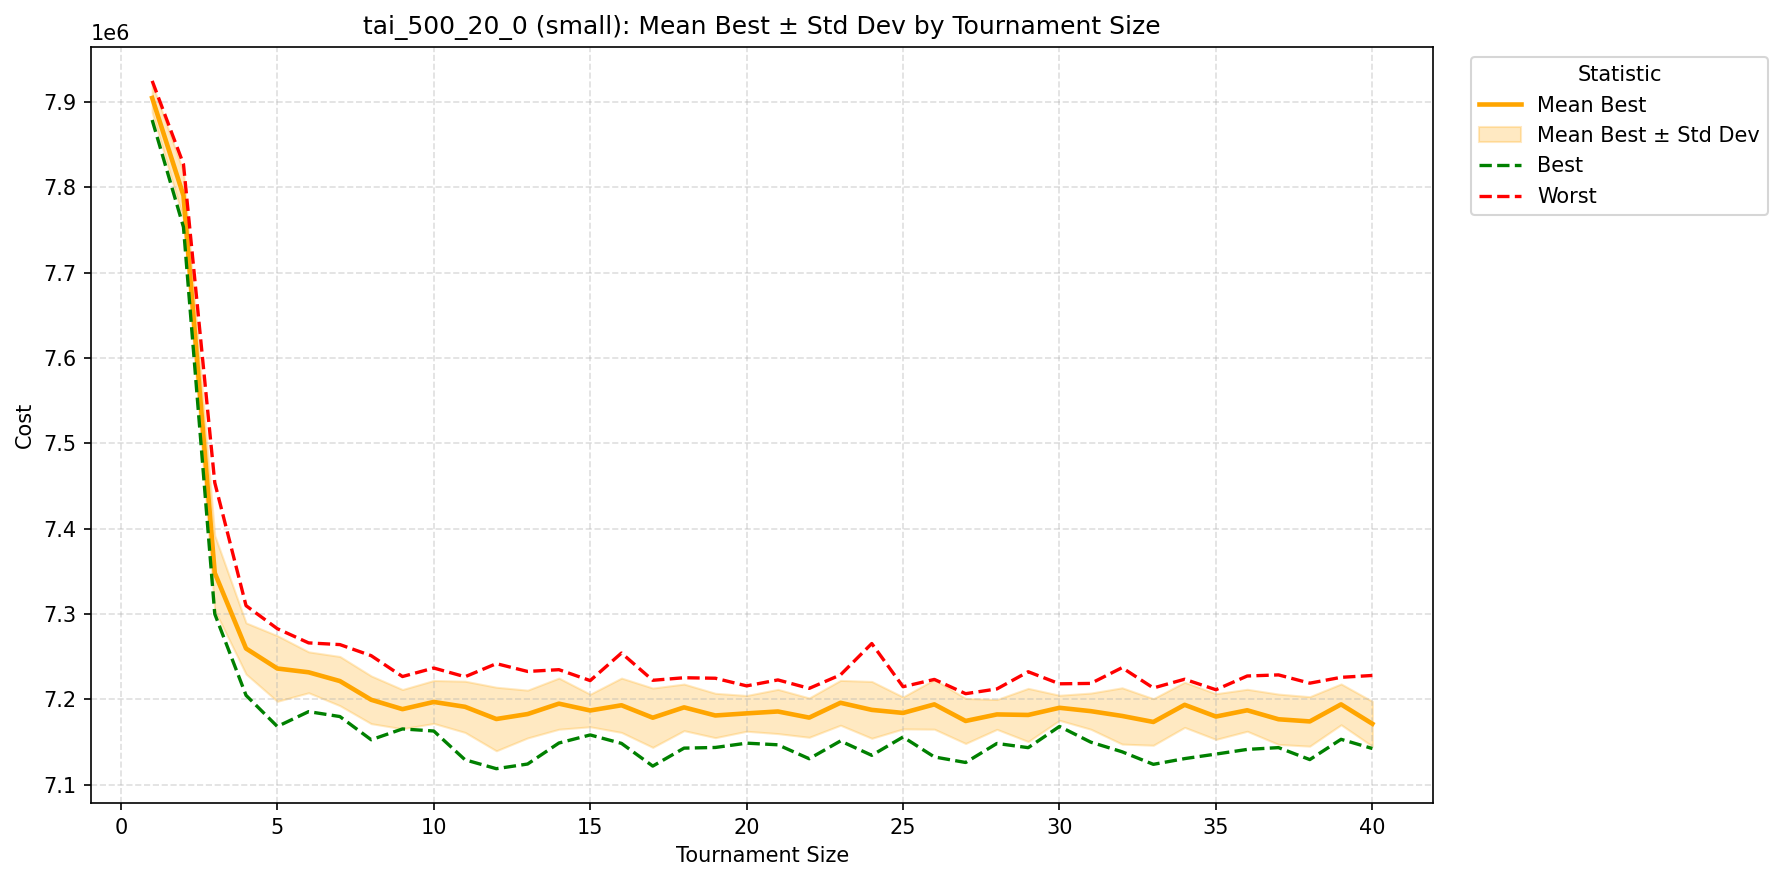
\includegraphics[width=0.48\textwidth]{../Experiments/06_evolutionary_tournament_grid/fig_tournament_tai_500_20_0.png}
\caption{Tournament size sensitivity for large instances (\texttt{tai\_100\_*}, \texttt{tai\_500\_20\_0}).}
\label{fig:tournament_large}
\end{figure}


\chapter{Implementation Details}



\subsection*{RandomSearchAlgorithm}
Pure random search: sample permutation, evaluate, keep best. Parameters: \texttt{EvaluationBudget}, \texttt{Seed}, monitoring.

\subsection*{GreedyAlgorithm and SptAlgorithm}
\texttt{GreedyAlgorithm} sorts jobs by total processing time and returns that order. \texttt{SptAlgorithm} inserts each next SPT-ordered job at the best position. Both are deterministic constructive baselines.

\subsection*{SimulatedAnnealingAlgorithm}
Starts from a random permutation. Each iteration generates a neighbor, evaluates it, applies acceptance, then updates temperature. Main parameters: \texttt{Iterations}, temperature settings, cooling schedule, neighborhood operator, acceptance function, \texttt{Seed}, \texttt{EvaluationBudget}.

\subsection*{EvolutionaryAlgorithm}
Maintains current and next populations. Uses tournament selection, OX/CX crossover, swap/insert mutation, and optional elitism (\texttt{ElitismK}). Main parameters: \texttt{PopulationSize}, \texttt{Generations}, \texttt{CrossoverRate}, \texttt{MutationRate}, \texttt{TournamentSize}, \texttt{ElitismK}, operators, \texttt{Seed}, \texttt{EvaluationBudget}.

\subsubsection*{Evolutionary Algorithm Operators}
\textbf{Selection:} Tournament selection is implemented, with size set by \texttt{TournamentSize} and pluggable via \texttt{SelectionMethod}.

\textbf{Crossover:} Supports Order Crossover (OX) and Cycle Crossover (CX), both pluggable via \texttt{CrossoverMethod}. OX copies a segment from one parent and fills the rest in order; CX identifies cycles and exchanges them.

\textbf{Mutation:} Supports Swap Mutation (swaps two jobs) and Insert Mutation (removes and reinserts a job), both pluggable via \texttt{MutationMethod}.

Operators are configured via parameters and run directly in the generational loop.

\section{Total Flow Time Evaluator}
Computes TFT with dynamic programming using a one-dimensional completion-time buffer.

\section{Experiment Runner}
The Experiment Runner executes reproducible experiment batches. It loads configs (JSON/CLI), expands algorithm-instance-parameter combinations, applies seeds, runs jobs across CPU cores, and saves structured JSON outputs.


\section{Monitoring and Metrics}
Monitoring uses \texttt{AlgorithmMonitor} to track start, candidate evaluation, generation/iteration events, and finish. Metrics (evaluations, elapsed time, best-so-far, convergence) are configured via \texttt{Monitoring}, stored in \texttt{AlgorithmResult}, and exported for analysis.


\section{Programming-Level Performance Optimizations Implemented}

\subsection*{Implementation-Specific Details}
\begin{itemize}
    \item \textbf{Evaluator hot loop:} \texttt{TotalFlowTimeEvaluator.Evaluate} uses a one-dimensional buffer (\texttt{comp}) for completion times, a per-machine row accessor (\texttt{Instance.GetMachineRow(int)}), and a direct conditional (\texttt{up > left ? up : left}) instead of \texttt{Math.Max} for speed.
    \item \textbf{Buffer pooling:} Temporary arrays for completion times are rented from \texttt{ArrayPool<double>} to reduce allocation and GC pressure.
    \item \textbf{Stack allocation:} In \texttt{EvolutionaryAlgorithm}, elitism selection uses \texttt{stackalloc} (\texttt{Span<bool>}) for the \texttt{taken} flags, avoiding heap allocations in the generational loop.
    \item \textbf{Operator profiling:} Profiling after evaluator optimizations identified crossover (especially Order Crossover) as a new hotspot, guiding further optimization focus.
    \item \textbf{Benchmark wiring:} ExperimentRunner and AlgorithmFactory ensure correct parameter grid expansion, seed distribution, and reproducible measurement scenarios.
\end{itemize}
Profiling repeatedly showed
\texttt{PFSP.Evaluators.TotalFlowTimeEvaluator.Evaluate(...)} as the main hotspot. The optimizations listed above were implemented from those traces.

\paragraph{Implementation references (files and line ranges).}
\begin{itemize}
    \item \texttt{PFSP/Instances/Instance.cs}: lines 69--76 (\texttt{GetMachineRow(int)}).
    \item \texttt{PFSP/Evaluators/TotalFlowTimeEvaluator.cs}: lines 27--82 (pooled buffer usage),
    lines 35--66 (row-based access and conditional max in inner loops).
    \item \texttt{PFSP/Algorithms/Evolutionary/EvolutionaryAlgorithm.cs}: line 53 (\texttt{stackalloc} buffer),
    lines 64--73 (elitism selection using stack-allocated \texttt{taken}).
    \item \texttt{ExperimentRunner/AlgorithmFactory.cs}: lines 47--74 (parameter-grid expansion),
    lines 168--187 (pairwise expansion), lines 88--93 (seed distribution by iteration).
\end{itemize}



\end{document}
